% Options for packages loaded elsewhere
\PassOptionsToPackage{unicode}{hyperref}
\PassOptionsToPackage{hyphens}{url}
%
\documentclass[
]{book}
\usepackage{amsmath,amssymb}
\usepackage{iftex}
\ifPDFTeX
  \usepackage[T1]{fontenc}
  \usepackage[utf8]{inputenc}
  \usepackage{textcomp} % provide euro and other symbols
\else % if luatex or xetex
  \usepackage{unicode-math} % this also loads fontspec
  \defaultfontfeatures{Scale=MatchLowercase}
  \defaultfontfeatures[\rmfamily]{Ligatures=TeX,Scale=1}
\fi
\usepackage{lmodern}
\ifPDFTeX\else
  % xetex/luatex font selection
\fi
% Use upquote if available, for straight quotes in verbatim environments
\IfFileExists{upquote.sty}{\usepackage{upquote}}{}
\IfFileExists{microtype.sty}{% use microtype if available
  \usepackage[]{microtype}
  \UseMicrotypeSet[protrusion]{basicmath} % disable protrusion for tt fonts
}{}
\makeatletter
\@ifundefined{KOMAClassName}{% if non-KOMA class
  \IfFileExists{parskip.sty}{%
    \usepackage{parskip}
  }{% else
    \setlength{\parindent}{0pt}
    \setlength{\parskip}{6pt plus 2pt minus 1pt}}
}{% if KOMA class
  \KOMAoptions{parskip=half}}
\makeatother
\usepackage{xcolor}
\usepackage{color}
\usepackage{fancyvrb}
\newcommand{\VerbBar}{|}
\newcommand{\VERB}{\Verb[commandchars=\\\{\}]}
\DefineVerbatimEnvironment{Highlighting}{Verbatim}{commandchars=\\\{\}}
% Add ',fontsize=\small' for more characters per line
\usepackage{framed}
\definecolor{shadecolor}{RGB}{248,248,248}
\newenvironment{Shaded}{\begin{snugshade}}{\end{snugshade}}
\newcommand{\AlertTok}[1]{\textcolor[rgb]{0.94,0.16,0.16}{#1}}
\newcommand{\AnnotationTok}[1]{\textcolor[rgb]{0.56,0.35,0.01}{\textbf{\textit{#1}}}}
\newcommand{\AttributeTok}[1]{\textcolor[rgb]{0.13,0.29,0.53}{#1}}
\newcommand{\BaseNTok}[1]{\textcolor[rgb]{0.00,0.00,0.81}{#1}}
\newcommand{\BuiltInTok}[1]{#1}
\newcommand{\CharTok}[1]{\textcolor[rgb]{0.31,0.60,0.02}{#1}}
\newcommand{\CommentTok}[1]{\textcolor[rgb]{0.56,0.35,0.01}{\textit{#1}}}
\newcommand{\CommentVarTok}[1]{\textcolor[rgb]{0.56,0.35,0.01}{\textbf{\textit{#1}}}}
\newcommand{\ConstantTok}[1]{\textcolor[rgb]{0.56,0.35,0.01}{#1}}
\newcommand{\ControlFlowTok}[1]{\textcolor[rgb]{0.13,0.29,0.53}{\textbf{#1}}}
\newcommand{\DataTypeTok}[1]{\textcolor[rgb]{0.13,0.29,0.53}{#1}}
\newcommand{\DecValTok}[1]{\textcolor[rgb]{0.00,0.00,0.81}{#1}}
\newcommand{\DocumentationTok}[1]{\textcolor[rgb]{0.56,0.35,0.01}{\textbf{\textit{#1}}}}
\newcommand{\ErrorTok}[1]{\textcolor[rgb]{0.64,0.00,0.00}{\textbf{#1}}}
\newcommand{\ExtensionTok}[1]{#1}
\newcommand{\FloatTok}[1]{\textcolor[rgb]{0.00,0.00,0.81}{#1}}
\newcommand{\FunctionTok}[1]{\textcolor[rgb]{0.13,0.29,0.53}{\textbf{#1}}}
\newcommand{\ImportTok}[1]{#1}
\newcommand{\InformationTok}[1]{\textcolor[rgb]{0.56,0.35,0.01}{\textbf{\textit{#1}}}}
\newcommand{\KeywordTok}[1]{\textcolor[rgb]{0.13,0.29,0.53}{\textbf{#1}}}
\newcommand{\NormalTok}[1]{#1}
\newcommand{\OperatorTok}[1]{\textcolor[rgb]{0.81,0.36,0.00}{\textbf{#1}}}
\newcommand{\OtherTok}[1]{\textcolor[rgb]{0.56,0.35,0.01}{#1}}
\newcommand{\PreprocessorTok}[1]{\textcolor[rgb]{0.56,0.35,0.01}{\textit{#1}}}
\newcommand{\RegionMarkerTok}[1]{#1}
\newcommand{\SpecialCharTok}[1]{\textcolor[rgb]{0.81,0.36,0.00}{\textbf{#1}}}
\newcommand{\SpecialStringTok}[1]{\textcolor[rgb]{0.31,0.60,0.02}{#1}}
\newcommand{\StringTok}[1]{\textcolor[rgb]{0.31,0.60,0.02}{#1}}
\newcommand{\VariableTok}[1]{\textcolor[rgb]{0.00,0.00,0.00}{#1}}
\newcommand{\VerbatimStringTok}[1]{\textcolor[rgb]{0.31,0.60,0.02}{#1}}
\newcommand{\WarningTok}[1]{\textcolor[rgb]{0.56,0.35,0.01}{\textbf{\textit{#1}}}}
\usepackage{longtable,booktabs,array}
\usepackage{calc} % for calculating minipage widths
% Correct order of tables after \paragraph or \subparagraph
\usepackage{etoolbox}
\makeatletter
\patchcmd\longtable{\par}{\if@noskipsec\mbox{}\fi\par}{}{}
\makeatother
% Allow footnotes in longtable head/foot
\IfFileExists{footnotehyper.sty}{\usepackage{footnotehyper}}{\usepackage{footnote}}
\makesavenoteenv{longtable}
\usepackage{graphicx}
\makeatletter
\def\maxwidth{\ifdim\Gin@nat@width>\linewidth\linewidth\else\Gin@nat@width\fi}
\def\maxheight{\ifdim\Gin@nat@height>\textheight\textheight\else\Gin@nat@height\fi}
\makeatother
% Scale images if necessary, so that they will not overflow the page
% margins by default, and it is still possible to overwrite the defaults
% using explicit options in \includegraphics[width, height, ...]{}
\setkeys{Gin}{width=\maxwidth,height=\maxheight,keepaspectratio}
% Set default figure placement to htbp
\makeatletter
\def\fps@figure{htbp}
\makeatother
\setlength{\emergencystretch}{3em} % prevent overfull lines
\providecommand{\tightlist}{%
  \setlength{\itemsep}{0pt}\setlength{\parskip}{0pt}}
\setcounter{secnumdepth}{5}
\usepackage{booktabs}
\usepackage{amsthm}
\makeatletter
\def\thm@space@setup{%
  \thm@preskip=8pt plus 2pt minus 4pt
  \thm@postskip=\thm@preskip
}
\makeatother
\ifLuaTeX
  \usepackage{selnolig}  % disable illegal ligatures
\fi
\usepackage[]{natbib}
\bibliographystyle{apalike}
\IfFileExists{bookmark.sty}{\usepackage{bookmark}}{\usepackage{hyperref}}
\IfFileExists{xurl.sty}{\usepackage{xurl}}{} % add URL line breaks if available
\urlstyle{same}
\hypersetup{
  pdftitle={Temas Selectos de Análisis Numérico y Computación Científica: Computo científico para el análisis de datos},
  pdfauthor={Haydeé Peruyero},
  hidelinks,
  pdfcreator={LaTeX via pandoc}}

\title{Temas Selectos de Análisis Numérico y Computación Científica: Computo científico para el análisis de datos}
\author{Haydeé Peruyero}
\date{2024-03-01}

\begin{document}
\maketitle

{
\setcounter{tocdepth}{1}
\tableofcontents
}
\hypertarget{temas-selectos-de-anuxe1lisis-numuxe9rico-y-computaciuxf3n-cientuxedfica-computo-cientuxedfico-para-el-anuxe1lisis-de-datos}{%
\chapter{Temas Selectos de Análisis Numérico y Computación Científica: Computo científico para el análisis de datos}\label{temas-selectos-de-anuxe1lisis-numuxe9rico-y-computaciuxf3n-cientuxedfica-computo-cientuxedfico-para-el-anuxe1lisis-de-datos}}

Curso del posgrado conjunto en Ciencias Matemáticas PCCM UNAM UMICH 2024-2

\hypertarget{temario}{%
\section{Temario}\label{temario}}

\begin{enumerate}
\def\labelenumi{\arabic{enumi}.}
\item
  Git y Github
\item
  Shell
\item
  Python
\item
  SQL
\item
  Power BI
\item
  R
\item
  Estadística multivariada
\item
  Análisis de regresión
\end{enumerate}

\hypertarget{referencias}{%
\section{Referencias}\label{referencias}}

{[}1{]} Arnold, Jeremey. Learning Microsoft Power BI, O'Reilly Media, Inc.

{[}2{]} Beaulieu, Alan. Learning SQL, O'Reilly Media, Inc., 2020

{[}3{]} Bruce, Peter, Bruce, Andrew and Gedeck, Peter. Practical Statistics for Data Scientists, O'Reilly Media, Inc., 2020.

{[}4{]} Crawley, Michael J. The R book. John Wiley \& Sons, 2012.

{[}5{]} McKinney, Wes. Python for data analysis. O'Reilly Media, Inc., 2022.

{[}6{]} Nelli, Fabio. Python Data Analytics, Apress.

{[}7{]} Wade, Ryan. Advanced Analytics in Power BI with R and Python, Apress.

{[}8{]} Wickham, Hadley, and Garrett Grolemund. R for data science: import, tidy, transform, visualize, and
model data. O Reilly Media, Inc., 2016.

{[}9{]} Zamora Saiz, Alfonso, et al.~An Introduction to Data Analysis in R: Hands-on Coding, Data Mining,
Visualization and Statistics from Scratch., Springer (2020).

{[}10{]} Software Carpentry, The Unix Shell, \url{https://swcarpentry.github.io/shell-novice/}

\hypertarget{material-interesante}{%
\section{Material interesante}\label{material-interesante}}

\begin{itemize}
\tightlist
\item
  \href{https://bookdown.org/}{Bookdown}.
\item
  \href{https://swcarpentry.github.io/r-novice-gapminder/}{Software Carpentry}.
\item
  \href{https://swcarpentry.github.io/git-novice/14-supplemental-rstudio/}{Git}
\item
  \href{https://info5940.infosci.cornell.edu/setup/git/what-is-git/}{Why Git}
\item
  \href{https://bookdown.org/yihui/rmarkdown-cookbook/}{R Markdown Cookbook}
\item
  \href{http://www.sthda.com/english/wiki/data-visualization}{STHDA}
\item
  \href{https://bookdown.org/ndphillips/YaRrr/}{YaRrr! The Pirate's Guide to R}
\item
  \href{https://link.springer.com/book/10.1007/978-3-319-53019-2}{Learn ggplot2 Using Shiny App}
\item
  \href{https://link.springer.com/book/10.1007/978-0-387-98141-3}{Ggplot2: Elegant Graphics for Data Analysis}

  \begin{itemize}
  \tightlist
  \item
    \href{https://ggplot2-book.org/index.html}{Versión online}
  \end{itemize}
\item
  \href{https://www.springer.com/series/6991/books}{Use R! Colección Springer}
\item
  \href{https://link.springer.com/book/10.1007/978-0-387-75969-2}{Lattice: Multivariate Data Visualization with R}
\item
  \href{http://www.cookbook-r.com/}{R Graphics cookbook}
\item
  \href{https://education.github.com/benefits}{Cuenta pro de Github}
\end{itemize}

\hypertarget{datacamp}{%
\section{DataCamp}\label{datacamp}}

\begin{figure}
\centering

\includegraphics{img/regular.png}
\caption{DataCamp}
\end{figure}

\hypertarget{shell}{%
\chapter{Shell}\label{shell}}

Descargar \href{https://gitforwindows.org/}{git bash} para Windows o seguir las instrucciones de \href{https://carpentries.github.io/workshop-template/install_instructions/\#shell}{Software carpentries} para otros sistemas operativos.
Basado en la lección de \href{https://swcarpentry.github.io/shell-novice/}{The carpentries}

\hypertarget{navegar-en-archivos-y-directorios}{%
\section{Navegar en archivos y directorios}\label{navegar-en-archivos-y-directorios}}

Cuando abrimos una terminal por primera vez, vamos a ver un \textbf{prompt} (usualmente es \texttt{\$}) que nos indica que esta esperando los comandos. Después de teclear los comandos, debemos siempre presionar Enter.

\begin{Shaded}
\begin{Highlighting}[]
\ExtensionTok{$} 
\end{Highlighting}
\end{Shaded}

Para listar lo que hay en un directorio usamos el comando \texttt{ls}.

\begin{Shaded}
\begin{Highlighting}[]
\ExtensionTok{$}\NormalTok{ ls}
\end{Highlighting}
\end{Shaded}

\begin{Shaded}
\begin{Highlighting}[]
\NormalTok{Documents  Downloads  Music  Pictures  Videos}
\end{Highlighting}
\end{Shaded}

Al comando \texttt{ls} le podemos agregar unos \texttt{adjetivos} para hacer más comprensible su lectura. Por ejemplo, la opción \texttt{-F} nos indica si es una carpeta, un archivo, un link, etc.

\begin{Shaded}
\begin{Highlighting}[]
\ExtensionTok{$}\NormalTok{ ls }\AttributeTok{{-}F}
\end{Highlighting}
\end{Shaded}

\begin{Shaded}
\begin{Highlighting}[]
\NormalTok{ej.txt  Git/  PBI/  Python/  R/  Shell/  SQL/}
\end{Highlighting}
\end{Shaded}

Con la opción \texttt{-\/-help} podemos acceder a la ayuda del comando.

\begin{Shaded}
\begin{Highlighting}[]
\ExtensionTok{$}\NormalTok{ ls }\AttributeTok{{-}{-}help}
\end{Highlighting}
\end{Shaded}

Otras opciones que nos ayudan a entender la información que tenemos en el archivo son \texttt{-lh}, nos muestra los permisos del archivo o carpeta, tamaño, propietario, fecha, nombre. La opción \texttt{ls\ -a} nos muestra los archivos ocultos.

\textbf{Ejercicio:} ¿Qué hace la opción \texttt{-l}? ¿Cómo podemos listar en orden de creación e inverso?

Con el comando \texttt{ls} también podemos listar los archivos de cualquier otro directorio, solo debemos indicarle el directorio después del comando:

\begin{Shaded}
\begin{Highlighting}[]
\ExtensionTok{$}\NormalTok{ ls }\AttributeTok{{-}}\NormalTok{ F Shell }
\end{Highlighting}
\end{Shaded}

El comando \texttt{ls} solo nos esta listando lo que hay en los directorios. Si nos queremos mover a otro directorio, lo podemos hacer con el comando \texttt{cd} y especificando el directorio.

\begin{Shaded}
\begin{Highlighting}[]
\ExtensionTok{$}\NormalTok{ cd Shell}
\ExtensionTok{$}\NormalTok{ ls}
\end{Highlighting}
\end{Shaded}

\begin{Shaded}
\begin{Highlighting}[]
\NormalTok{data/  ej1.txt  ejercicios/}
\end{Highlighting}
\end{Shaded}

El comando \texttt{pwd} nos da la ruta en la que estamos.

\begin{Shaded}
\begin{Highlighting}[]
\ExtensionTok{$}\NormalTok{ pwd}
\end{Highlighting}
\end{Shaded}

\begin{Shaded}
\begin{Highlighting}[]
\NormalTok{/d/Users/hayde/Documents/Curso\_Comp\_Cien/Shell}
\end{Highlighting}
\end{Shaded}

Para movernos a un directorio arriba, colocamos después de \texttt{cd} dos puntos.

\begin{Shaded}
\begin{Highlighting}[]
\ExtensionTok{$}\NormalTok{ cd ..}
\end{Highlighting}
\end{Shaded}

Si no colocamos los dos puntos, el comando \texttt{cd} nos lleva al \texttt{/home/}.

\begin{Shaded}
\begin{Highlighting}[]
\ExtensionTok{$}\NormalTok{ cd }
\end{Highlighting}
\end{Shaded}

Otra forma de movernos de un directorio a otro es especificando la \emph{ruta absoluta}, es decir la ruta completa de a donde queremos movernos.

\begin{Shaded}
\begin{Highlighting}[]
\ExtensionTok{$}\NormalTok{ cd /d/Users/hayde/Documents/Curso\_comp\_Cien}
\end{Highlighting}
\end{Shaded}

\textbf{Ejercicio:} ¿Qué es una ruta relativa?

Otro opción útil que podemos usar con el comando \texttt{cd} es \texttt{-}.

\textbf{Ejercicio:} ¿A donde nos lleva \texttt{cd\ -}? y si volvemos a colocar \texttt{cd\ -} ¿a donde nos lleva? ¿Cuál es la diferencia entre \texttt{cd\ ..} y \texttt{cd\ -}?

La tilde \texttt{\textasciitilde{}}, shell la interpreta como el home del usuario, entonces si colocamos \texttt{cd\ \textasciitilde{}/directorio} sería lo mismo que \texttt{/home/directorio}. Por ejemplo:

\begin{Shaded}
\begin{Highlighting}[]
\ExtensionTok{$}\NormalTok{ cd \textasciitilde{}/Desktop}
\end{Highlighting}
\end{Shaded}

es lo mismo que

\begin{Shaded}
\begin{Highlighting}[]
\ExtensionTok{$}\NormalTok{ cd /c/Users/hayde/Desktop}
\end{Highlighting}
\end{Shaded}

\textbf{Ejercicio:} Supongamos que tenemos el siguiente árbol de datos en nuestra computadora y que estamos en \texttt{/Users/thing/}. ¿Si colocamos en la terminal \texttt{ls\ -F\ ../backup} que nos mostrará?

\begin{figure}
\centering
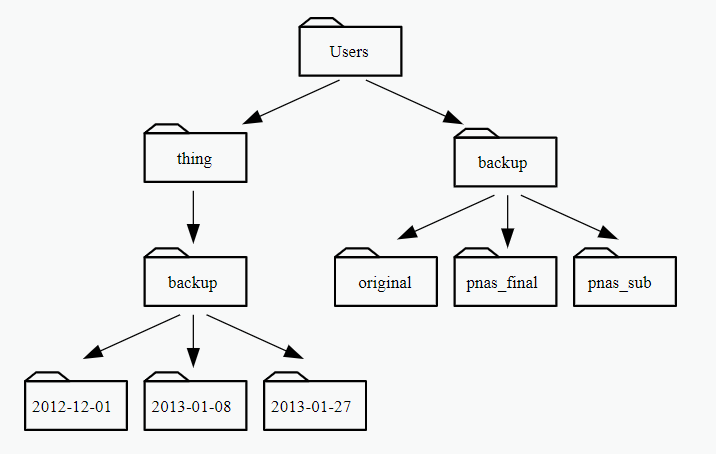
\includegraphics{img/ej_shell.png}
\caption{Ejercicio \href{https://swcarpentry.github.io/shell-novice/02-filedir.html}{SC}}
\end{figure}

\textbf{Ejercicio:} Explora las opciones \texttt{-s} y \texttt{-S}. ¿Hay diferencia entre mayúsculas y minúsculas?

La tecla Tab nos ayuda a completar los comando/rutas. Si la presionamos dos veces nos mostrará todas las posibles opciones.

\hypertarget{manipulaciuxf3n-de-archivos-y-directorios}{%
\section{Manipulación de archivos y directorios}\label{manipulaciuxf3n-de-archivos-y-directorios}}

Para crear directorios/carpetas desde la línea de comandos usamos el comando \texttt{mkdir\ nombre}. Vamos a crear la carpeta del curso. Es recomendable \textbf{no usar espacios en nombres de carpetas ni archivos}.

\begin{Shaded}
\begin{Highlighting}[]
\ExtensionTok{$}\NormalTok{ mkdir Curso\_Comp\_Cien}
\end{Highlighting}
\end{Shaded}

El comando \texttt{mkdir} nos permite crear más de un directorio y directorios anidados usando la opción \texttt{-p}.

\begin{Shaded}
\begin{Highlighting}[]
\ExtensionTok{$}\NormalTok{ mkdir }\AttributeTok{{-}p}\NormalTok{ Curso\_Comp\_Cien/Shell/data Curso\_Comp\_Cien/Shell/ejercicios}
\end{Highlighting}
\end{Shaded}

Para listar toda la estructura de nuestras carpetas podemos usar la opción \texttt{-FR} en el comando \texttt{ls}.

\begin{Shaded}
\begin{Highlighting}[]
\ExtensionTok{$}\NormalTok{ ls }\AttributeTok{{-}FR}
\end{Highlighting}
\end{Shaded}

Otra opción útil para listar toda la estructura de nuestro directorio es la opción \texttt{tree}, no viene instalado por default en los sistemas operativos. En Windows, si se instalo git/bash se puede usar con \texttt{tree.com}.

\begin{Shaded}
\begin{Highlighting}[]
\ExtensionTok{$}\NormalTok{ tree.com}
\end{Highlighting}
\end{Shaded}

\textbf{Nota:} Para descargar \texttt{tree} y que podamos ver la estructura de árbol con archivos y carpetas hacer lo siguiente:

\begin{enumerate}
\def\labelenumi{\arabic{enumi})}
\item
  Ir a la \href{https://gnuwin32.sourceforge.net/packages/tree.htm}{página} y descargar la versión que dice \emph{binaries}.
\item
  Extraer lo que hay en la carpeta \textbf{bin}.
\item
  Copiar el archivo \textbf{tree.exe} a la carpeta \texttt{/c/Program\_files/Git/usr/bin/}.
\item
  Para probarlo, solo colocar en la terminal \texttt{tree\ ruta}.
\end{enumerate}

Para crear un archivo usando el editor nano (si fue el que configuraron), se usa el comando \texttt{nano\ nombre.extension}.
Vamos a crear un archivo de prueba en la carpeta ejercicios y escribamos algo en el archivo.

\begin{Shaded}
\begin{Highlighting}[]
\ExtensionTok{$}\NormalTok{ cd Curso\_Comp\_Cien/}
\ExtensionTok{$}\NormalTok{ nano prueba.txt}
\end{Highlighting}
\end{Shaded}

Para guardar y salir del editor, usamos los comandos Ctrl+O o Ctrl+X seguido de \texttt{Yes} y enter.

Si en el archivo no guardaron nada, entonces no se creara. Una forma de crear archivos sin abrirlos es con el comando \texttt{touch}.

\begin{Shaded}
\begin{Highlighting}[]
\ExtensionTok{$}\NormalTok{ cd Shell/ejercicios}
\ExtensionTok{$}\NormalTok{ touch ../ej1.txt ej2.txt ../data/ej3.csv ../data/ej4.csv}
\end{Highlighting}
\end{Shaded}

Si checamos con \texttt{ls\ -l} los archivos o rutas que creamos, veremos que no tienen ningún tamaño.

Para mover archivos o renombrarlos, usamos el comando \texttt{mv} seguido del archivo que queremos mover/renombrar y la ruta a donde lo moveremos o el nuevo nombre del archivo.

\begin{Shaded}
\begin{Highlighting}[]
\ExtensionTok{$}\NormalTok{ pwd}
\ExtensionTok{$}\NormalTok{ mv ej2.txt ejercicio2.txt}
\end{Highlighting}
\end{Shaded}

Lo anterior esta cambiándole el nombre al archivo \texttt{ej2.txt} por \texttt{ejercicio2.txt}.

Si estamos en un directorio y queremos mover un archivo de otro directorio al directorio actual, podemos hacerlo especificando como primer argumento la ruta y nombre del archivo a mover y como segundo argumento un punto \texttt{.}.

\begin{Shaded}
\begin{Highlighting}[]
\ExtensionTok{$}\NormalTok{ mv ../ej1.txt .}
\end{Highlighting}
\end{Shaded}

O especificando la ruta completa.

\begin{Shaded}
\begin{Highlighting}[]
\ExtensionTok{$}\NormalTok{ cd ..}
\ExtensionTok{$}\NormalTok{ mv data/ej3.csv ejercicios/.}
\end{Highlighting}
\end{Shaded}

Para copiar archivos, usamos el comando \texttt{cp} seguido por la ruta del archivo a copiar y la ruta del archivo a donde se copiará. Movámonos a la carpeta \texttt{Shell/ejercicios}.

\begin{Shaded}
\begin{Highlighting}[]
\ExtensionTok{$}\NormalTok{ pwd}
\ExtensionTok{$}\NormalTok{ cp ejercicio2.txt ../ej2.txt}
\ExtensionTok{$}\NormalTok{ ls }\AttributeTok{{-}FR}
\end{Highlighting}
\end{Shaded}

Si usamos la opción \texttt{-r} (\emph{recursivo}) en el comando \texttt{cp} podemos copiar un directorio completo y todos sus elementos.

\begin{Shaded}
\begin{Highlighting}[]
\ExtensionTok{$}\NormalTok{ cd ejercicios}
\ExtensionTok{$}\NormalTok{ cp }\AttributeTok{{-}r}\NormalTok{ ../data .}
\end{Highlighting}
\end{Shaded}

Si el último parámetro de \texttt{cp} es un directorio que ya existe, entonces copiará todos los archivos que se indiquen a ese directorio. Por ejemplo:

\begin{Shaded}
\begin{Highlighting}[]
\ExtensionTok{$}\NormalTok{ cp archivo1.txt archivo2.txt data}
\end{Highlighting}
\end{Shaded}

De igual forma para \texttt{mv}, si el último parámetro es un directorio movera todos los archivos a ese directorio.

\begin{Shaded}
\begin{Highlighting}[]
\ExtensionTok{$}\NormalTok{ mv archivo1.txt archivo2.txt data}
\end{Highlighting}
\end{Shaded}

\textbf{Ejercicio:} ¿Cual es el output de la siguiente colección de comandos?

\begin{Shaded}
\begin{Highlighting}[]
\ExtensionTok{$}\NormalTok{ pwd}
\end{Highlighting}
\end{Shaded}

\begin{Shaded}
\begin{Highlighting}[]
\NormalTok{/Users/haydee/Curso}
\end{Highlighting}
\end{Shaded}

\begin{Shaded}
\begin{Highlighting}[]
\ExtensionTok{$}\NormalTok{ ls }\AttributeTok{{-}F}
\end{Highlighting}
\end{Shaded}

\begin{Shaded}
\begin{Highlighting}[]
\NormalTok{archivo.txt carpeta/}
\end{Highlighting}
\end{Shaded}

\begin{Shaded}
\begin{Highlighting}[]
\ExtensionTok{$}\NormalTok{ mkdir carpeta2}
\ExtensionTok{$}\NormalTok{ mv archivo.txt carpeta2/}
\ExtensionTok{$}\NormalTok{ cd carpeta2}
\ExtensionTok{$}\NormalTok{ cp archivo.txt ../carpeta/archivo\_respaldo.txt}
\ExtensionTok{$}\NormalTok{ cd ..}
\ExtensionTok{$}\NormalTok{ ls }\AttributeTok{{-}FR}
\end{Highlighting}
\end{Shaded}

Para borrar archivos usamos el comando \texttt{rm}, hay que tener cuidado cuando lo usemos ya que \textbf{borra definitivamente} los archivos o carpetas.

\begin{Shaded}
\begin{Highlighting}[]
\ExtensionTok{$}\NormalTok{ cd Shell}
\ExtensionTok{$}\NormalTok{ rm ejercicios/ejercicio2.txt}
\ExtensionTok{$}\NormalTok{ ls ejercicios/}
\end{Highlighting}
\end{Shaded}

Una forma segura de borrar archivos es usando la opción \texttt{-i}, con esto nos saldrá un mensaje preguntando si en verdad deseamos borrar el archivo. Para confirmar debemos colocar \texttt{y}.

\begin{Shaded}
\begin{Highlighting}[]
\ExtensionTok{$}\NormalTok{ rm }\AttributeTok{{-}i}\NormalTok{ /data/ej3.csv}
\end{Highlighting}
\end{Shaded}

\begin{Shaded}
\begin{Highlighting}[]
\NormalTok{rm: remove regular empty file \textquotesingle{}ej3.txt\textquotesingle{}?}
\end{Highlighting}
\end{Shaded}

Si queremos borrar una carpeta, debemos hacerlo con la opción \texttt{-r}, de lo contrario obtendremos un error.

\begin{Shaded}
\begin{Highlighting}[]
\ExtensionTok{$}\NormalTok{ rm data}
\end{Highlighting}
\end{Shaded}

\begin{Shaded}
\begin{Highlighting}[]
\ExtensionTok{$}\NormalTok{ rm }\AttributeTok{{-}r}\NormalTok{ data}
\end{Highlighting}
\end{Shaded}

Otra opción para borrar directorios es \texttt{rmdir}.

Para mover/copiar/eliminar multiples archivos a la vez, podemos enumerarlos todos o usar comodines/patrones que sigan estos elementos. Supongamos que tenemos una lista de archivos todos con terminación \texttt{.txt}, entonces para borrarlos podemos usar \texttt{rm\ *.txt}. El \texttt{*} nos indica todo lo que este antes de \texttt{.txt}.

\begin{Shaded}
\begin{Highlighting}[]
\ExtensionTok{$}\NormalTok{ cd Shell/}
\ExtensionTok{$}\NormalTok{ touch prueba1.txt prueba2.txt prueba3.txt prueba4.txt prueba5.txt}
\ExtensionTok{$}\NormalTok{ rm }\PreprocessorTok{*}\NormalTok{.txt}
\end{Highlighting}
\end{Shaded}

Otro comodín que podemos usar es \texttt{?}, pero este denota solo 1 espacio. Por ejemplo:

\begin{Shaded}
\begin{Highlighting}[]
\ExtensionTok{$}\NormalTok{ cd Shell/}
\ExtensionTok{$}\NormalTok{ touch prueba1.txt prueba2.txt prueba3.txt prueba4.txt prueba5.txt}
\ExtensionTok{$}\NormalTok{ rm prueba}\PreprocessorTok{?}\NormalTok{.txt}
\end{Highlighting}
\end{Shaded}

\begin{Shaded}
\begin{Highlighting}[]
\ExtensionTok{$}\NormalTok{ cd Shell/}
\ExtensionTok{$}\NormalTok{ touch prueba1.txt prueba2.txt prueba3.txt prueba4.txt prueba5.txt}
\ExtensionTok{$}\NormalTok{ rm prue}\PreprocessorTok{???}\NormalTok{.txt}
\end{Highlighting}
\end{Shaded}

\textbf{Ejercicio:} Supon que en el directorio \texttt{data} tienes dos archivos. ¿Cuál de los siguientes comandos te daría como resultado: \texttt{ethane.pdb} \texttt{methane.pdb}.

\begin{enumerate}
\def\labelenumi{\arabic{enumi})}
\item
  \texttt{ls\ *t*ane.pdb}
\item
  \texttt{ls\ *t?ne.*}
\item
  \texttt{ls\ *t??ne.pdb}
\item
  ls ethane.*
\end{enumerate}

Dos comodines más que existen son los siguientes:

\begin{itemize}
\item
  \texttt{{[}...{]}}: busca coincidencias con exactamente cada caracter dentro de los corchetes, por ejemplo \texttt{{[}12{]}} coincidiria con \texttt{texto1.txt}, \texttt{texto2.tx} pero no con \texttt{texto3.txt}.
\item
  \texttt{\{...\}}: busca coincidencias con cada uno de los elementos separados por comas dentro de las llaves, por ejemplo \texttt{\{*.txt,\ *.csv\}} buscaría todos los archivos con terminaciones \texttt{.txt} y \texttt{.csv} pero no con los que sean \texttt{.pdf}.
\end{itemize}

\hypertarget{tuberuxedas-y-filtros}{%
\section{Tuberías y filtros}\label{tuberuxedas-y-filtros}}

Vamos a usar los archivos de prueba de la lección de Shell de Software Carpentry. Descargarlos en el directorio que creamos que se llama \href{https://swcarpentry.github.io/shell-novice/data/shell-lesson-data.zip}{Shell}.

Vamos a explorar los archivos que están en la carpeta \texttt{excercise-data/alkanes}. Para contar cuantos palabras, líneas o caracteres tiene un archivo, usamos el comando \texttt{wc} que viene de \texttt{word\ count}.

\begin{Shaded}
\begin{Highlighting}[]
\ExtensionTok{$}\NormalTok{ ls}
\end{Highlighting}
\end{Shaded}

\begin{Shaded}
\begin{Highlighting}[]
\NormalTok{cubane.pdb  ethane.pdb  methane.pdb  octane.pdb  pentane.pdb  propane.pdb}
\end{Highlighting}
\end{Shaded}

\begin{Shaded}
\begin{Highlighting}[]
\ExtensionTok{$}\NormalTok{ wc cubane.pdb}
\end{Highlighting}
\end{Shaded}

\begin{Shaded}
\begin{Highlighting}[]
\NormalTok{20  156 1158 cubane.pdb}
\end{Highlighting}
\end{Shaded}

El primer número es el número de líneas del archivo, el segundo la cantidad de palabras y el tercero la cantidad de caracteres.

Si usamos alguna de los comodines, por ejemplo \texttt{*.pdb} con el comando \texttt{wc}, nos va a regresar la información de todos los archivos.

\begin{Shaded}
\begin{Highlighting}[]
\ExtensionTok{$}\NormalTok{ wc }\PreprocessorTok{*}\NormalTok{.pdb}
\end{Highlighting}
\end{Shaded}

Notemos que en la última fila tenemos los totales de todos los archivos. Accedamos a la ayuda del comando con \texttt{help}.

\begin{Shaded}
\begin{Highlighting}[]
\ExtensionTok{$}\NormalTok{ wc }\AttributeTok{{-}{-}help}
\end{Highlighting}
\end{Shaded}

\textbf{Ejercicio:} ¿Cuál opción nos permite extraer solo la cantidad de líneas del archivo?

\begin{Shaded}
\begin{Highlighting}[]
\ExtensionTok{$}\NormalTok{ wc }\AttributeTok{{-}l} \PreprocessorTok{*}\NormalTok{.pdb}
\end{Highlighting}
\end{Shaded}

Si por error olvidamos colocar el nombre del archivo o cualquier otra cosa después del comando, la consola se quedará esperando una instrucción, para salir de esto basta presionar Ctrl+C.

Ya sabemos como extraer cierta información de nuestros archivos, pero supongamos que queremos guardarlo ahora en algún otro archivo para después analizarlo. El símbolo \texttt{\textgreater{}} redirige el resultado de los comandos usados a algún archivo.

\begin{Shaded}
\begin{Highlighting}[]
\ExtensionTok{$}\NormalTok{ wc }\AttributeTok{{-}l} \PreprocessorTok{*}\NormalTok{.pdb }\OperatorTok{\textgreater{}}\NormalTok{ lineas.txt}
\end{Highlighting}
\end{Shaded}

Para solo visualizar el contenido de un archivo sin entrar al editor de texto, podemos usar el comando \texttt{cat} seguido del nombre del archivo.

\begin{Shaded}
\begin{Highlighting}[]
\ExtensionTok{$}\NormalTok{ cat lineas.txt}
\end{Highlighting}
\end{Shaded}

Otro comando que puede resultar más útil para mostrar el contenido de un archivo es \texttt{less}, la diferencia con \texttt{cat} es que este último muestra todo el contenido en la pantalla, lo cual puede dificultar su lectura e inspección, mientras que \texttt{less} muestra una parte del contenido y de forma ordenada, si queremos seguir viendo el contenido podemos usar la tecla de espacio, b y para salir usamos la letra \texttt{q}.

Ya guardamos la información de la cantidad de líneas, pero supongamos que queremos saber cual archivo tiene la mayor cantidad de líneas o menor. Para hacer esto nos sirve el comando \texttt{sort}.

\begin{Shaded}
\begin{Highlighting}[]
\ExtensionTok{$}\NormalTok{ cd ..}
\ExtensionTok{$}\NormalTok{ sort numbers.txt}
\end{Highlighting}
\end{Shaded}

Si a \texttt{sort} le agregamos la opción \texttt{-n}, nos los ordena en numericamente en lugar de alfabeticamente.

\begin{Shaded}
\begin{Highlighting}[]
\ExtensionTok{$}\NormalTok{ sort }\AttributeTok{{-}n}\NormalTok{ numbers.txt}
\end{Highlighting}
\end{Shaded}

\textbf{Ejercicio:} De los archivos que están en la carpeta \texttt{alkane}, ¿cuál tiene la menor cantidad de líneas?

También podemos redirigir esta información a otro archivo y de ahí extraer la información.

\begin{Shaded}
\begin{Highlighting}[]
\ExtensionTok{$}\NormalTok{ sort }\AttributeTok{{-}n}\NormalTok{ lineas.txt }\OperatorTok{\textgreater{}}\NormalTok{ lineas\_ordenadas.txt}
\end{Highlighting}
\end{Shaded}

El comando \texttt{head} nos ayuda a extraer las primeras \texttt{n} líneas de nuestro archivo. Por ejemplo, para extraer la primera línea del archivo \texttt{lineas\_ordenadas.txt} y así saber cual archivo tenía la menor cantidad de líneas usaríamos \texttt{head\ -n\ 1}.

\begin{Shaded}
\begin{Highlighting}[]
\ExtensionTok{$}\NormalTok{ head }\AttributeTok{{-}n}\NormalTok{ 1 lineas\_ordenadas.txt}
\end{Highlighting}
\end{Shaded}

El comando \texttt{echo} nos ayuda a imprimir en la consola caracteres.

\begin{Shaded}
\begin{Highlighting}[]
\ExtensionTok{$}\NormalTok{ echo Hola}
\end{Highlighting}
\end{Shaded}

\textbf{Ejercicio:} Realiza las siguientes instrucciones dos veces cada una. Explora las diferencias. ¿Qué hace el operador \texttt{\textgreater{}\textgreater{}}?

\begin{Shaded}
\begin{Highlighting}[]
\ExtensionTok{$}\NormalTok{ echo hola }\OperatorTok{\textgreater{}}\NormalTok{ test1.txt}
\end{Highlighting}
\end{Shaded}

\begin{Shaded}
\begin{Highlighting}[]
\ExtensionTok{$}\NormalTok{ echo hola }\OperatorTok{\textgreater{}\textgreater{}}\NormalTok{ test2.txt}
\end{Highlighting}
\end{Shaded}

El comando \texttt{tail} es similar al comando \texttt{head}, nos muestra las últimas \texttt{n} filas del archivo.

\textbf{Ejercicio:} Considera el archivo \texttt{/exercise-data/animal-counts/animals.csv}. Después de aplicar los siguientes dos comandos, ¿qué hay en el archivo \texttt{animals-subset.csv}?

\begin{Shaded}
\begin{Highlighting}[]
\ExtensionTok{$}\NormalTok{ head }\AttributeTok{{-}n}\NormalTok{ 3 animals.csv }\OperatorTok{\textgreater{}}\NormalTok{ animals{-}subset.csv}
\ExtensionTok{$}\NormalTok{ tail }\AttributeTok{{-}n}\NormalTok{ 2 animals.csv }\OperatorTok{\textgreater{}\textgreater{}}\NormalTok{ animals{-}subset.csv}
\end{Highlighting}
\end{Shaded}

\hypertarget{tuberuxedas}{%
\subsection{Tuberías}\label{tuberuxedas}}

Además de redirigir los output de los comandos que hemos ocupado, también podríamos anidarlos y al final mandarlo a un archivo. Para hacer esto se usan \textbf{tuberías} y su símbolo es \texttt{\textbar{}}. Por ejemplo:

\begin{Shaded}
\begin{Highlighting}[]
\ExtensionTok{$}\NormalTok{ sort }\AttributeTok{{-}n}\NormalTok{ lineas.txt }\KeywordTok{|} \FunctionTok{head} \AttributeTok{{-}n}\NormalTok{ 1}
\end{Highlighting}
\end{Shaded}

En esta instrucción le estamos diciendo a la consola que primero nos ordene lo que hay en el archivo líneas en orden númerico y después que nos muestre la primera línea. De esta forma nos evitamos por ejemplo el haber creado el archivo \texttt{lineas\_ordenadas.txt}.

Podemos anidar varias instrucciones a la vez. Por ejemplo, podríamos pedirle a la consola la cantidad de líneas de los archivos \texttt{*.pdb}, pedirle que las ordene numericamente y después que extraiga la primera línea.

\begin{Shaded}
\begin{Highlighting}[]
\ExtensionTok{$}\NormalTok{ wc }\AttributeTok{{-}l} \PreprocessorTok{*}\NormalTok{.pdb }\KeywordTok{|} \FunctionTok{sort} \AttributeTok{{-}n} \KeywordTok{|} \FunctionTok{head} \AttributeTok{{-}n}\NormalTok{ 1}
\end{Highlighting}
\end{Shaded}

\textbf{Ejercicio:} De los archivos que están en la carpeta \texttt{alkanes}, obten los 3 archivos con la menor cantidad de líneas.

\textbf{Ejercicio:} Explora el archivo \texttt{exercise-data/animals-counts/animals.csv}. ¿Cuál será el resultado de la siguiente instrucción?

\begin{Shaded}
\begin{Highlighting}[]
\ExtensionTok{$}\NormalTok{ cat animals.csv }\KeywordTok{|} \FunctionTok{head} \AttributeTok{{-}n}\NormalTok{ 5 }\KeywordTok{|} \FunctionTok{tail} \AttributeTok{{-}n}\NormalTok{ 3 }\KeywordTok{|} \FunctionTok{sort} \AttributeTok{{-}r} \OperatorTok{\textgreater{}}\NormalTok{ final.txt}
\end{Highlighting}
\end{Shaded}

El comando \texttt{cut} nos ayuda a extrar/cortar ciertas columnas de nuestros archivos. Por ejemplo, \texttt{cut\ -d\ ,\ -f\ 2\ archivo} nos está indicando que del archivo queremos cortar por caracteres \texttt{,} (eso hace \texttt{-d\ ,}) y que queremos extraer la segunda columna (\texttt{-f\ 2}).

\begin{Shaded}
\begin{Highlighting}[]
\ExtensionTok{$}\NormalTok{ cut }\AttributeTok{{-}d}\NormalTok{ , }\AttributeTok{{-}f}\NormalTok{ 2 animals.csv}
\end{Highlighting}
\end{Shaded}

Si quisieramos extraer los animales únicos de ese archivo, podemos usar el comando \texttt{uniq}.

\begin{Shaded}
\begin{Highlighting}[]
\ExtensionTok{$}\NormalTok{ cut }\AttributeTok{{-}d}\NormalTok{ , }\AttributeTok{{-}f}\NormalTok{ 2 animals.csv }\KeywordTok{|} \FunctionTok{sort} \KeywordTok{|} \FunctionTok{uniq}
\end{Highlighting}
\end{Shaded}

También se puede colocar por ejemplo \texttt{-f\ 2-5,8} para indicar que se deben seleccionar las columnas 2 a la 5 y la 8.

\textbf{Ejercicio:} ¿Porqué se necesita colocar el \texttt{sort} antes del \texttt{uniq}?

\textbf{Ejercicio:} Si quisiéramos ver cuantos animales hay de cada tipo, ¿que instrucción tendríamos que usar?

\hypertarget{ciclos}{%
\section{Ciclos}\label{ciclos}}

Los ciclos nos ayudan a repetir comandos o un conjunto de comandos para cada elemento de una lista. La estructura del ciclo \texttt{for} es como sigue:

\begin{Shaded}
\begin{Highlighting}[]
\ControlFlowTok{for}\NormalTok{ elemento }\KeywordTok{in}\NormalTok{ lista}
\ControlFlowTok{do} 
  \ExtensionTok{operacion/comando} \VariableTok{$elemento}
\ControlFlowTok{done}
\end{Highlighting}
\end{Shaded}

La palabra \texttt{for} indica el comienzo del ciclo, la palabra \texttt{do} nos indica que es lo que se va a ejecutar y su comienzo y la palabra \texttt{done} indica el fin del ciclo.

Exploremos lo que hay en la carpeta \texttt{\textasciitilde{}/Shell/shell-lesson-data/exercise-data/creatures}. Listemos las primeras 5 filas de cada archivo.

\begin{Shaded}
\begin{Highlighting}[]
\ExtensionTok{$}\NormalTok{ head }\AttributeTok{{-}n}\NormalTok{ 5 basilisk.dat minotaur.dat unicorn.dat}
\end{Highlighting}
\end{Shaded}

Supongamos que queremos ver la clasificación de cada especie que se encuentra en la segunda línea de cada archivo. Una forma de hacerlo es con \texttt{head\ -n\ 2}, pero de esta forma también estamos viendo su nombre común, entonces vamos a hacerlo con un ciclo. Lo primero que tendríamos que hacer es usar justo \texttt{head\ -n\ 2} y al resultado de esto, si le pedimos la última línea ya solo veríamos la clasificación, entonces usamos un \texttt{tail\ -n\ 1}.

\begin{Shaded}
\begin{Highlighting}[]
\ExtensionTok{$}\NormalTok{ for filename in }\PreprocessorTok{*}\NormalTok{.dat}
\OperatorTok{\textgreater{}}\NormalTok{ do}
\OperatorTok{\textgreater{}}\NormalTok{   echo }\VariableTok{$filename}
\OperatorTok{\textgreater{}}\NormalTok{   head }\ExtensionTok{{-}n}\NormalTok{ 2 }\VariableTok{$filename} \KeywordTok{|} \FunctionTok{tail} \AttributeTok{{-}n}\NormalTok{ 1}
\OperatorTok{\textgreater{}}\NormalTok{ done}
\end{Highlighting}
\end{Shaded}

Notemos que cuando empezamos a teclear nuestro ciclo, el prompt cambia de \texttt{\$} a \texttt{\textgreater{}}, esto indica que está esperando que continuemos el ciclo. También podemos usar \texttt{;} para continuar las instrucciones en una misma fila.

Dentro de los ciclos, las variables las mandamos a llamar con \texttt{\$}, en el ejemplo, cuando ocupamos \texttt{\$filename} estamos mandando a llamar la variable \texttt{filename} que definimos al inicio del ciclo. Es muy usual también encerrar entre llaves los nombres de las variables para delimitar el nombre, en el ejemplo, \texttt{\$filename} sería equivalente a \texttt{\$\{filename\}}.

\textbf{Ejercicio:} Crea un ciclo que muestre en pantalla (echo) todos los números del 0 al 9.

\textbf{Ejercicio:} Ve a la carpeta \texttt{shell-lesson-data/exercise-data/alkanes} y lista lo que hay.
1) ¿Cuál es el output del siguiente código?

\begin{Shaded}
\begin{Highlighting}[]
\ExtensionTok{$}\NormalTok{ for datafile in }\PreprocessorTok{*}\NormalTok{.pdb}
\OperatorTok{\textgreater{}}\NormalTok{ do}
\OperatorTok{\textgreater{}}\NormalTok{     ls }\ExtensionTok{*.pdb}
\OperatorTok{\textgreater{}}\NormalTok{ done}
\end{Highlighting}
\end{Shaded}

\begin{enumerate}
\def\labelenumi{\arabic{enumi})}
\setcounter{enumi}{1}
\tightlist
\item
  ¿Y de este código?
\end{enumerate}

\begin{Shaded}
\begin{Highlighting}[]
\ExtensionTok{$}\NormalTok{ for datafile in }\PreprocessorTok{*}\NormalTok{.odb}
\OperatorTok{\textgreater{}}\NormalTok{ do }
\OperatorTok{\textgreater{}}\NormalTok{     ls }\VariableTok{$datafile}
\OperatorTok{\textgreater{}}\NormalTok{ done}
\end{Highlighting}
\end{Shaded}

Explica las diferencias.

\textbf{Ejercicio:} En el directorio \texttt{shell-lesson-data/exercise-data/alkanes}, ¿cuál sería el output del siguiente código?

\begin{Shaded}
\begin{Highlighting}[]
\ExtensionTok{$}\NormalTok{ for filename in c}\PreprocessorTok{*}
\OperatorTok{\textgreater{}}\NormalTok{ do}
\OperatorTok{\textgreater{}}\NormalTok{     ls }\VariableTok{$filename}
\OperatorTok{\textgreater{}}\NormalTok{ done}
\end{Highlighting}
\end{Shaded}

Y si en lugar de \texttt{c*} usamos \emph{c}?

Dentro de un ciclo también podemos pedir guardar archivos.

\textbf{Ejercicio:} Explora el siguiente código. ¿Cuál es el efecto de guardar en este ciclo?

\begin{Shaded}
\begin{Highlighting}[]
\ExtensionTok{$}\NormalTok{ for alkanes in }\PreprocessorTok{*}\NormalTok{.pdb}
\OperatorTok{\textgreater{}}\NormalTok{ do}
\OperatorTok{\textgreater{}}\NormalTok{     echo }\VariableTok{$alkanes}
\OperatorTok{\textgreater{}}\NormalTok{     cat }\VariableTok{$alkanes} \OperatorTok{\textgreater{}}\NormalTok{ alkanes.pdb}
\OperatorTok{\textgreater{}}\NormalTok{ done}
\end{Highlighting}
\end{Shaded}

¿Cuál sería la diferencia si usamos ahora \texttt{\textgreater{}\textgreater{}}?

\textbf{Ejercicio:} Crea un ciclo que muestre las últimas 20 líneas de cada archivo en la carpeta \texttt{creatures}.

Como ya mencionamos, no es recomendable usar espacios ni caracteres especiales en nombres de archivos o carpetas. Si fuera el caso de que nuestros archivos tienen espacios, entonces deberíamos pasarlos al ciclo for encerrados entre comillas los nombres. Por ejemplo, supongamos que tenemos los archivos \texttt{archivo\ 1.txt} y \texttt{archivo\ 2.txt}. Para leerlos en el ciclo for tendríamos que usar la siguiente sintaxis.

\begin{Shaded}
\begin{Highlighting}[]
\ExtensionTok{$}\NormalTok{ for filename in }\StringTok{"archivo 1.txt"} \StringTok{"archivo 2.txt"}
\OperatorTok{\textgreater{}}\NormalTok{ do}
\OperatorTok{\textgreater{}}\NormalTok{     head }\ExtensionTok{{-}n20} \StringTok{"}\VariableTok{$filename}\StringTok{"} \KeywordTok{|} \FunctionTok{tail} \AttributeTok{{-}n5} 
\OperatorTok{\textgreater{}}\NormalTok{ done}
\end{Highlighting}
\end{Shaded}

Supongamos que queremos modificar nuestros archivos que se encuentran en la carpeta \texttt{creatures} pero que antes queremos respaldarlos en otros archivos llamados \texttt{original-basilisk.dat}, \texttt{original-unicorn.dat} y \texttt{original-minotaur.dat}. Una forma de hacerlo sería copiarlos a nuevos archivos con esos nombres, pero si no lo queremos hacer manualmente, ¿qué pasa si usamos el siguiente código?

\begin{Shaded}
\begin{Highlighting}[]
\ExtensionTok{$}\NormalTok{ cp }\PreprocessorTok{*}\NormalTok{.dat original{-}}\PreprocessorTok{*}\NormalTok{.dat}
\end{Highlighting}
\end{Shaded}

Esto nos va a dar un error porque el comando \texttt{cp} estaría esperando que \texttt{original-} sea una carpeta y no lo es, no existe esa carpeta. Entonces lo que podemos hacer es usar un ciclo.

\textbf{Ejercicio:} Crea un ciclo \texttt{for} que copie los dos archivos a dos nuevos archivos llamados \texttt{original-basilisk.dat}, \texttt{original-unicorn.dat} y \texttt{original-minotaur.dat}.

El comando \texttt{cp} no nos muestra en pantalla ningún output. Si quisieramos ver que en efecto se esta realizando la copia de estos archivos podemos usar el comando \texttt{echo} y pedir que nos diga como ``se copio el archivo \$filename''. Usar \texttt{echo} de esta forma es una buena práctica de realizar lo que se llama \textbf{debugging}.

\begin{Shaded}
\begin{Highlighting}[]
\ExtensionTok{$}\NormalTok{ for filename in }\PreprocessorTok{*}\NormalTok{.dat}
\OperatorTok{\textgreater{}}\NormalTok{ do}
\OperatorTok{\textgreater{}}\NormalTok{     echo }\FunctionTok{cp} \VariableTok{$filename}\NormalTok{ original{-}}\VariableTok{$filename}
\OperatorTok{\textgreater{}}\NormalTok{ done}
\end{Highlighting}
\end{Shaded}

\begin{figure}
\centering
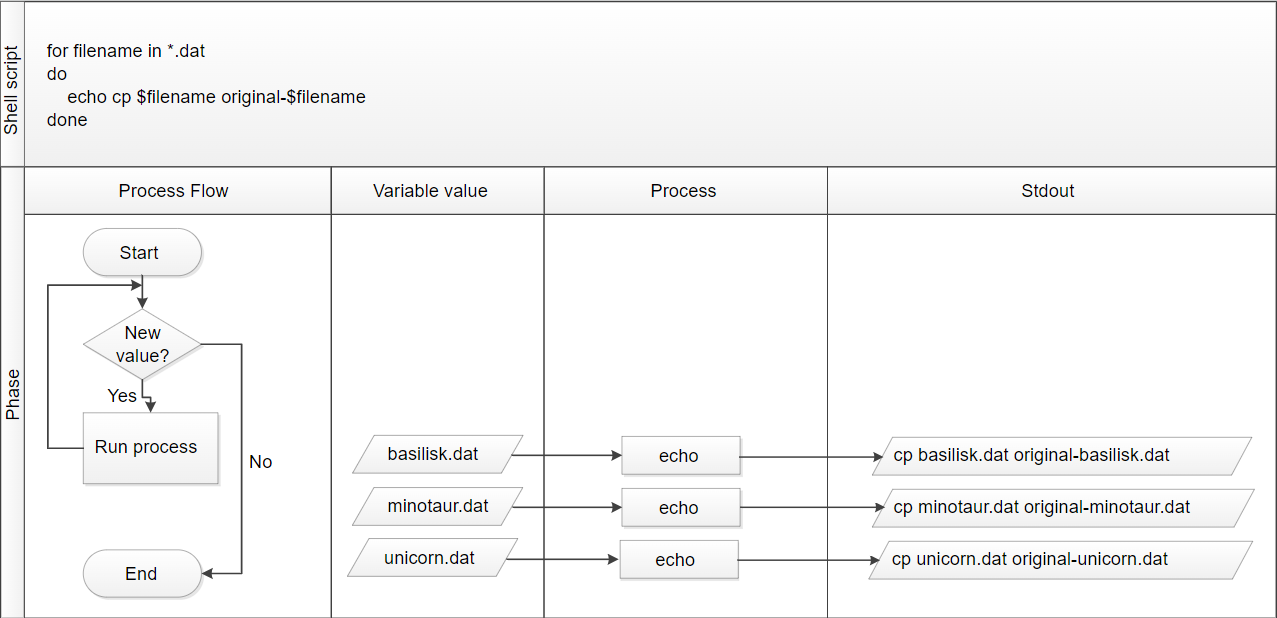
\includegraphics{D:/Users/hayde/Documents/R_sites/Computo_Cientifico/img/shell_script_for_loop_flow_chart.png}
\caption{Debugging}
\end{figure}

\textbf{Ejercicio:} Supongamos que queremos previsualizar los comandos que el siguiente ciclo va a realizar en lugar de correrlo primero para asegurarnos de que está haciendo lo que queremos.

\begin{Shaded}
\begin{Highlighting}[]
\ExtensionTok{$}\NormalTok{ for filename in }\PreprocessorTok{*}\NormalTok{.pdb}
\OperatorTok{\textgreater{}}\NormalTok{ do}
\OperatorTok{\textgreater{}}\NormalTok{     cat }\VariableTok{$filename} \OperatorTok{\textgreater{}\textgreater{}}\NormalTok{ all.pdb}
\OperatorTok{\textgreater{}}\NormalTok{ done}
\end{Highlighting}
\end{Shaded}

¿Cuál de los siguientes dos códigos sería el correcto para revisar los comando a ejecutarse con el ciclo?

\begin{Shaded}
\begin{Highlighting}[]
\CommentTok{\# Versión 1}
\ExtensionTok{$}\NormalTok{ for filename in }\PreprocessorTok{*}\NormalTok{.pdb}
\OperatorTok{\textgreater{}}\NormalTok{ do}
\OperatorTok{\textgreater{}}\NormalTok{     echo }\FunctionTok{cat} \VariableTok{$filename} \OperatorTok{\textgreater{}\textgreater{}}\NormalTok{ all.pdb}
\OperatorTok{\textgreater{}}\NormalTok{ done}
\end{Highlighting}
\end{Shaded}

\begin{Shaded}
\begin{Highlighting}[]
\CommentTok{\# Versión 2}
\ExtensionTok{$}\NormalTok{ for filename in }\PreprocessorTok{*}\NormalTok{.pdb}
\OperatorTok{\textgreater{}}\NormalTok{ do}
\OperatorTok{\textgreater{}}\NormalTok{    echo }\StringTok{"cat }\VariableTok{$filename}\StringTok{ \textgreater{}\textgreater{} all.pdb"}
\OperatorTok{\textgreater{}}\NormalTok{ done}
\end{Highlighting}
\end{Shaded}

Corre los dos códigos y explora el contenido del archivo \texttt{all.pdb}.

Supongamos que queremos crear una estructura de directorios como sigue, para cada compuesto y cada temperatura queremos una carpeta para ir guardando ahí sus resultados, y que cada carpeta se llame \texttt{compuesto-temperatura}, ¿cómo podemos hacer esto? Una opción son los ciclos anidados.

\begin{figure}
\centering
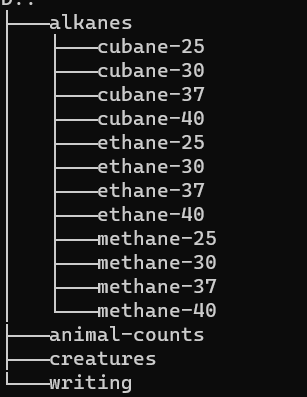
\includegraphics{D:/Users/hayde/Documents/R_sites/Computo_Cientifico/img/estructura-alkanes.png}
\caption{estructura-experimentos}
\end{figure}

\begin{Shaded}
\begin{Highlighting}[]
\ExtensionTok{$}\NormalTok{ for species in cubane ethane methane }
\OperatorTok{\textgreater{}}\NormalTok{ do}
\OperatorTok{\textgreater{}}\NormalTok{     for }\ExtensionTok{temperature}\NormalTok{ in 25 30 37 40}
\OperatorTok{\textgreater{}}\NormalTok{     do}
\OperatorTok{\textgreater{}}\NormalTok{         mkdir }\VariableTok{$species}\ExtensionTok{{-}}\VariableTok{$temperature}
\OperatorTok{\textgreater{}}\NormalTok{     done}
\OperatorTok{\textgreater{}}\NormalTok{ done}
\end{Highlighting}
\end{Shaded}

Algunos comandos útiles para ver el historial de comadnos.

\begin{itemize}
\item
  \texttt{history} nos muestra el historial de comandos.
\item
  Ctrl+R nos muestra la leyenda \texttt{reverse-i-search}, esto indica que está esperando que nosotros coloquemos una palabra y buscará por el último comando con esa palabra.
\item
  \texttt{history} + \texttt{!123} nos repetirá el comando \texttt{!123} del historial.
\item
  \texttt{!!} nos muestra el último comando usado.
\item
  \texttt{!\$} nos regresa la última palabra del último comando.
\end{itemize}

\textbf{Ejercicio:} En la carpeta \texttt{norht-pacific-gyre} se encuentran dos scripts (\texttt{.sh}) y una lista de archivos. Esta lista de archivos tiene terminaciones A, B y en el caso de que la terminación sea Z significa que el archivo está corrupto.

\begin{enumerate}
\def\labelenumi{\arabic{enumi})}
\tightlist
\item
  ¿Cómo podrías darte cuenta que los archivos con terminación Z están corruptos?
\end{enumerate}

Supongamos que queremos ejecutar el script llamado \texttt{goostats.sh}, este script necesita recibir dos cosas, el archivo de entrada y el nombre del archivo de salida. Supongamos que queremos correr este script para todos los archivos con terminación A y B y que queremos que los archivos de salida se llamen \texttt{stats-\$datafile}.

\begin{enumerate}
\def\labelenumi{\arabic{enumi})}
\setcounter{enumi}{1}
\item
  Crea un ciclo que te muestre en pantalla el nombre del archivo a usar como input.
\item
  Crea un ciclo que te muestre en pantalla el nombre del archivo de salida con el formato indicado. Pero quieres asegurarte que para el archivo input sea el nombre correcto el del archivo de salida.
\item
  Crea un ciclo que muestre los comandos a usarse para correr el script con los archivos de entrada y de salida del paso 2 y 3. Para correr un script como se indica, se usa el comando \texttt{bash\ nombre\_archivo.sh\ input\ output}.
\item
  Agrega un \texttt{echo\ \$datafile} para saber en que archivo va tu ciclo.
\end{enumerate}

\hypertarget{scripts}{%
\section{Scripts}\label{scripts}}

Los scripts nos ayudan a repetir los comandos sobre listas de archivos. Supongamos que existen ciertos comando que siempre repetimos, vamos a guardarlos en un archivo para con un solo comando ejecutar esa lista de comandos.

Vamos al directorio \texttt{alkanes}. Supongamos que siempre queremos extraer las líneas de la 11 a la 15 de cada archivo. Por ejemplo, una forma en la que lo hacemos es:

\begin{Shaded}
\begin{Highlighting}[]
\ExtensionTok{$}\NormalTok{ head }\AttributeTok{{-}n}\NormalTok{ 15 octane.pdb }\KeywordTok{|} \FunctionTok{tail} \AttributeTok{{-}n}\NormalTok{ 5}
\end{Highlighting}
\end{Shaded}

Vamos a escribir eso en un archivo:

\begin{Shaded}
\begin{Highlighting}[]
\ExtensionTok{$}\NormalTok{ cd alkanes}
\ExtensionTok{$}\NormalTok{ nano middle.sh}
\end{Highlighting}
\end{Shaded}

Guardemos eso. Para ejecutarlo bastaría correr lo siguiente:

\begin{Shaded}
\begin{Highlighting}[]
\ExtensionTok{$}\NormalTok{ bash middle.sh}
\end{Highlighting}
\end{Shaded}

Supongamos que queremos las líneas de la 11 a la 15 pero de cualquier otro archivo. Vamos a modificar el archivo que creamos.

\begin{Shaded}
\begin{Highlighting}[]
\ExtensionTok{$}\NormalTok{ nano middle.sh}
\end{Highlighting}
\end{Shaded}

\begin{Shaded}
\begin{Highlighting}[]
\FunctionTok{head} \AttributeTok{{-}n}\NormalTok{ 15 }\StringTok{"}\VariableTok{$1}\StringTok{"} \KeywordTok{|} \FunctionTok{tail} \AttributeTok{{-}n}\NormalTok{ 5}
\end{Highlighting}
\end{Shaded}

En el script, cuando colocamos \texttt{"\$1"} se refiere al primer argumento/archivo en la línea de comandos, por ejemplo cuando colocamos en la línea de comandos:

\begin{Shaded}
\begin{Highlighting}[]
\ExtensionTok{$}\NormalTok{ bash middle.sh octane.pdb}
\end{Highlighting}
\end{Shaded}

Lo que estamos diciéndole a la consola es que reemplace dentro del script ``\$1'' por el archivo \texttt{octane.pdb}. De esta forma nuestro script ahora lo podemos correr sobre cualquier archivo.

Nuestro script por el momento funciona solo con las líneas de la 11 a la 15. Supongamos que queremos modificar esto de tal forma que cuando vayamos a ejecutar el script le indiquemos las líneas que queremos extraer. Así como usamos \texttt{\$1} para indicarle que era la primera variable en la línea de comandos, podemos usar las variables \texttt{\$2} y \texttt{\$3} para indicarle la segunda y tercera variable.

\begin{Shaded}
\begin{Highlighting}[]
\ExtensionTok{$}\NormalTok{ nano middle.sh}
\end{Highlighting}
\end{Shaded}

\begin{Shaded}
\begin{Highlighting}[]
\FunctionTok{head} \AttributeTok{{-}n} \StringTok{"}\VariableTok{$2}\StringTok{"} \StringTok{"}\VariableTok{$1}\StringTok{"} \KeywordTok{|} \FunctionTok{tail} \AttributeTok{{-}n} \StringTok{"}\VariableTok{$3}\StringTok{"}
\end{Highlighting}
\end{Shaded}

Entonces podemos ejecutar el script como sigue:

\begin{Shaded}
\begin{Highlighting}[]
\ExtensionTok{$}\NormalTok{ bash middle.sh octane.pdb 15 5}
\end{Highlighting}
\end{Shaded}

Y podemos cambiar las líneas a mostrar, por ejemplo:

\begin{Shaded}
\begin{Highlighting}[]
\ExtensionTok{$}\NormalTok{ bash middle.sh octane.pdb 20 5}
\end{Highlighting}
\end{Shaded}

Lo único que falta en el script, es describir que hace, de esta forma cualquier otra persona (o nosotros más adelante), cuando queramos abrir el script podamos recordar y entender que argumentos pide y cual es su uso.

\begin{Shaded}
\begin{Highlighting}[]
\ExtensionTok{$}\NormalTok{ nano middle.sh}
\end{Highlighting}
\end{Shaded}

\begin{Shaded}
\begin{Highlighting}[]
\CommentTok{\# Selecciona líneas intermedias de un archivo.}
\CommentTok{\# Uso: bash middle.sh nombre\_archivo linea\_final linea\_inicial}
\FunctionTok{head} \AttributeTok{{-}n} \StringTok{"}\VariableTok{$2}\StringTok{"} \StringTok{"}\VariableTok{$1}\StringTok{"} \KeywordTok{|} \FunctionTok{tail} \AttributeTok{{-}n} \StringTok{"}\VariableTok{$3}\StringTok{"}
\end{Highlighting}
\end{Shaded}

Ahora, supongamos que queremos ordenar los archivos \texttt{.pdb} por cantidad de líneas. Sin un script eso lo hacemos así:

\begin{Shaded}
\begin{Highlighting}[]
\ExtensionTok{$}\NormalTok{ wc }\AttributeTok{{-}l} \PreprocessorTok{*}\NormalTok{.pdb }\KeywordTok{|} \FunctionTok{sort} \AttributeTok{{-}n} 
\end{Highlighting}
\end{Shaded}

Si queremos poner esto en un script pero queremos correrlo sobre varios tipos de archivos, digamos los \texttt{.pdb} y los \texttt{.dat}, no podemos colocar en nuestro script \texttt{*.pdb}, y si usamos como en los ejemplos anteriores \texttt{"\$1"} o \texttt{"\$2}, eso limitaría la cantidad de archivos que podemos pasarle después en la consola. Una forma de no depender de eso es con la variable \texttt{\$@}, esto indica que pueden ser cualquier cantidad de argumentos en la línea de comandos.

\begin{Shaded}
\begin{Highlighting}[]
\ExtensionTok{$}\NormalTok{ nano sorted.sh}
\end{Highlighting}
\end{Shaded}

\begin{Shaded}
\begin{Highlighting}[]
\CommentTok{\# Ordena archivos por su longitud}
\CommentTok{\# Uso: bash sorted.sh uno\_o\_mas\_archivos}
\FunctionTok{wc} \AttributeTok{{-}l} \StringTok{"}\VariableTok{$@}\StringTok{"} \KeywordTok{|} \FunctionTok{sort} \AttributeTok{{-}n}
\end{Highlighting}
\end{Shaded}

\begin{Shaded}
\begin{Highlighting}[]
\ExtensionTok{$}\NormalTok{ bash sorted.sh }\PreprocessorTok{*}\NormalTok{.pdb ../creatures/}\PreprocessorTok{*}\NormalTok{.dat}
\end{Highlighting}
\end{Shaded}

\textbf{Ejercicio:} El archivo \texttt{animals.csv} ya vimos que es un archivo separado por comas que indica las especies y la cantidad de cada uno. Crea un script que se pueda aplicar a cualquier cantidad de archivos con ese formato y que te diga las especies únicas de cada archivo.
Crea 3 archivos similares al \texttt{animals.csv} (copia y modifica) y prueba tu script.

\textbf{Ejercicio:} Corre el siguiente comando:

\begin{Shaded}
\begin{Highlighting}[]
\ExtensionTok{$}\NormalTok{ history }\KeywordTok{|} \FunctionTok{tail} \AttributeTok{{-}n}\NormalTok{ 5 }\OperatorTok{\textgreater{}}\NormalTok{ recientes.sh}
\end{Highlighting}
\end{Shaded}

¿Qué contiene ese archivo? ¿Observa la última línea del archivo? ¿Porqué guarda esa línea?

\textbf{Ejercicio:} En la carpeta \texttt{alkanes} supongamos que tenemos un \texttt{script.sh} que contiene lo siguiente:

\begin{Shaded}
\begin{Highlighting}[]
\ExtensionTok{$}\NormalTok{ head }\AttributeTok{{-}n} \VariableTok{$2} \VariableTok{$1}
\ExtensionTok{$}\NormalTok{ tail }\AttributeTok{{-}n} \VariableTok{$3} \VariableTok{$1}
\end{Highlighting}
\end{Shaded}

Dentro del directorio \texttt{alkanes}, corre lo siguiente:

\begin{Shaded}
\begin{Highlighting}[]
\ExtensionTok{$}\NormalTok{ bash script.sh }\StringTok{\textquotesingle{}*.pdb\textquotesingle{}}\NormalTok{ 1 1}
\end{Highlighting}
\end{Shaded}

¿Qué esperas obtener?

\textbf{Ejercicio:} Crea un script llamado \texttt{longest.sh} que reciba como argumentos un directorio y una extensión de archivos y que te devuelva el archivo en el directorio, que tenga esa extensión, con el mayor número de líneas.

\textbf{Ejercicio:} Considera los archivos que están en la carpeta \texttt{alkanes}. Explica que hace cada uno de los siguientes scripts al correrlos como \texttt{bash\ script1.sh\ *.pdb}, \texttt{bash\ script2.sh\ *.pdb} y \texttt{bash\ script3.sh\ *.pdb}.

\begin{Shaded}
\begin{Highlighting}[]
\CommentTok{\# Script 1}
\BuiltInTok{echo} \PreprocessorTok{*}\NormalTok{.}\PreprocessorTok{*}
\end{Highlighting}
\end{Shaded}

\begin{Shaded}
\begin{Highlighting}[]
\CommentTok{\# Script 2}
\ControlFlowTok{for}\NormalTok{ filename }\KeywordTok{in} \VariableTok{$1} \VariableTok{$2} \VariableTok{$3}
\ControlFlowTok{do}
  \FunctionTok{cat} \VariableTok{$filename}
\ControlFlowTok{done}
\end{Highlighting}
\end{Shaded}

\begin{Shaded}
\begin{Highlighting}[]
\CommentTok{\# Script 3}
\BuiltInTok{echo} \VariableTok{$@}\NormalTok{.pdb}
\end{Highlighting}
\end{Shaded}

\textbf{Ejercicio:} (Debugging) Supongamos que tienen el siguiente script \texttt{do-errors.sh} en la carpeta \texttt{north-pacific-gyre}:

\begin{Shaded}
\begin{Highlighting}[]
\CommentTok{\# Calcular estadisticas para los archivos}
\ControlFlowTok{for}\NormalTok{ datafile }\KeywordTok{in} \StringTok{"}\VariableTok{$@}\StringTok{"}
\ControlFlowTok{do}
  \BuiltInTok{echo} \VariableTok{$datafile}
  \FunctionTok{bash}\NormalTok{ goostats.sh }\VariableTok{$datfile}\NormalTok{ stats{-}}\VariableTok{$datafile}
\ControlFlowTok{done}
\end{Highlighting}
\end{Shaded}

Corre en la línea de comandos:

\begin{Shaded}
\begin{Highlighting}[]
\ExtensionTok{$}\NormalTok{ bash do{-}errors.sh NENE}\PreprocessorTok{*}\NormalTok{A.txt NENE}\PreprocessorTok{*}\NormalTok{B.txt}
\end{Highlighting}
\end{Shaded}

No muestra ninguna salida. Para ver porque, vamos a correrlo de nuevo con la opción -x:

\begin{Shaded}
\begin{Highlighting}[]
\ExtensionTok{$}\NormalTok{ bash }\AttributeTok{{-}x}\NormalTok{ do{-}errors.sh NENE}\PreprocessorTok{*}\NormalTok{A.txt NENE}\PreprocessorTok{*}\NormalTok{B.txt}
\end{Highlighting}
\end{Shaded}

¿Cuál es el output? ¿Cuál es la línea responsable del error?

Otra asignación de variables es \texttt{\#@}, esto nos indica cuantos objetos hay de la variable.

Tres conceptos usados en bash son los siguientes:

\begin{itemize}
\item
  STDIN: estándar input
\item
  STDOUT: estándar output
\item
  STDERR: estándar error
\end{itemize}

Para redirigir el error y el output automáticamente a archivos, usamos las opciones:

\begin{Shaded}
\begin{Highlighting}[]
\ExtensionTok{$} \DecValTok{2}\OperatorTok{\textgreater{}}\NormalTok{ error.txt }\KeywordTok{\&} \DecValTok{1}\OperatorTok{\textgreater{}}\NormalTok{ output.txt}
\end{Highlighting}
\end{Shaded}

O dentro de un script:

\begin{Shaded}
\begin{Highlighting}[]
\BuiltInTok{exec} \DecValTok{1}\OperatorTok{\textgreater{}\textgreater{}}\NormalTok{ output.txt }\DecValTok{2}\OperatorTok{\textgreater{}\textgreater{}}\NormalTok{ error.txt}
\end{Highlighting}
\end{Shaded}

Al inicio de un script se suele colocar \texttt{\#!/usr/bash} para que el interprete sepa que es un script de bash y use el bash que se encuentra en \texttt{usr/bash}. Si no está ahí se coloca la ruta correspondiente, para saber donde está usamos \texttt{which\ bash}.

\hypertarget{buscando-y-encontrando-cosas}{%
\section{Buscando y encontrando cosas}\label{buscando-y-encontrando-cosas}}

La función \texttt{grep} (\emph{global/regular expression/print}) nos ayuda a encontrar e imprimir líneas de archivos que contengan un patrón especificado.

Vamos a la ruta \texttt{excercise-data/writing}.

\begin{Shaded}
\begin{Highlighting}[]
\ExtensionTok{$}\NormalTok{ cat haiku.txt}
\end{Highlighting}
\end{Shaded}

Para buscar las líneas que contienen la palabra \texttt{not}, la instrucción sería la siguiente:

\begin{Shaded}
\begin{Highlighting}[]
\ExtensionTok{$}\NormalTok{ grep not haiku.txt}
\end{Highlighting}
\end{Shaded}

El comando \texttt{grep} es sensible a mayúsculas y minúsculas. Si buscáramos por ejemplo \texttt{Not} no nos encontraría ninguna coincidencia.

\begin{Shaded}
\begin{Highlighting}[]
\ExtensionTok{$}\NormalTok{ grep The haiku.txt}
\end{Highlighting}
\end{Shaded}

Observemos que ahora nos está regresando una palabra que contiene \texttt{The} en su estructura: \texttt{Thesis}. Para restringir a que solo sean coincidencias exactas, usamos la bandera \texttt{-w}.

\begin{Shaded}
\begin{Highlighting}[]
\ExtensionTok{$}\NormalTok{ grep }\AttributeTok{{-}w}\NormalTok{ The haiuku.txt}
\end{Highlighting}
\end{Shaded}

En el caso de querer buscar frases, debemos encerrarlas entre comillas.

\begin{Shaded}
\begin{Highlighting}[]
\ExtensionTok{$}\NormalTok{ grep }\AttributeTok{{-}w} \StringTok{"is not"}\NormalTok{ haiku.txt}
\end{Highlighting}
\end{Shaded}

Si agregamos la opción \texttt{-n}, esto nos mostrará también la línea en la que se encuentra la coincidencia.

\begin{Shaded}
\begin{Highlighting}[]
\ExtensionTok{$}\NormalTok{ grep }\AttributeTok{{-}n} \StringTok{"it"}\NormalTok{ haiku.txt}
\end{Highlighting}
\end{Shaded}

Las banderas se pueden combinar, por ejemplo \texttt{-nw} (\texttt{-wn} o \texttt{-n\ -w}) nos buscaría coincidencias exactas y los números de líneas.

\begin{Shaded}
\begin{Highlighting}[]
\ExtensionTok{$}\NormalTok{ grep }\AttributeTok{{-}nw} \StringTok{"it"}\NormalTok{ haiku.txt}
\end{Highlighting}
\end{Shaded}

Para que no nos importe mayúsculas o minúsculas, usamos la opción \texttt{-i}.

\begin{Shaded}
\begin{Highlighting}[]
\ExtensionTok{$}\NormalTok{ grep }\AttributeTok{{-}n} \AttributeTok{{-}w} \AttributeTok{{-}i} \StringTok{"the"}\NormalTok{ haiku.txt}
\end{Highlighting}
\end{Shaded}

La opción \texttt{-v} es para invertir nuestra búsqueda, es decir para mostrarnos las líneas que no contienen esa palabra/frase.

\begin{Shaded}
\begin{Highlighting}[]
\ExtensionTok{$}\NormalTok{ grep }\AttributeTok{{-}n} \AttributeTok{{-}w} \AttributeTok{{-}v} \StringTok{"the"}\NormalTok{ haiku.txt}
\end{Highlighting}
\end{Shaded}

La opción \texttt{-r} busca recursivamente por la coincidencia en un conjunto de archivos indicados.

\begin{Shaded}
\begin{Highlighting}[]
\ExtensionTok{$}\NormalTok{ grep }\AttributeTok{{-}r}\NormalTok{ Yesterday .}
\end{Highlighting}
\end{Shaded}

\textbf{Ejercicio:} ¿Cómo obtendrían solo lo siguiente del archivo \texttt{haiku.txt}?

\begin{Shaded}
\begin{Highlighting}[]
\ExtensionTok{and}\NormalTok{ the presence of absence.}
\end{Highlighting}
\end{Shaded}

Dentro del comando \texttt{grep} también podemos usar comodines (expresiones regulares), por ejemplo:

\begin{Shaded}
\begin{Highlighting}[]
\ExtensionTok{$}\NormalTok{ grep }\AttributeTok{{-}E} \StringTok{"\^{}.o"}\NormalTok{ haiku.txt}
\end{Highlighting}
\end{Shaded}

El \texttt{\^{}} se refiere al inicio de la línea, el \texttt{.} se refiere a un carácter (análogo a \texttt{?}), entonces estaría buscando todas las líneas una palabra donde su segunda letra sea la letra \texttt{o}.

\textbf{Ejercicio:} El archivo que se encuentra en la carpeta \texttt{animal-counts/animals.csv} contiene una lista de animales, con su fecha de observación y cuantos animales se observaron.

\begin{Shaded}
\begin{Highlighting}[]
\NormalTok{2012{-}11{-}05,deer,5}
\NormalTok{2012{-}11{-}05,rabbit,22}
\NormalTok{2012{-}11{-}05,raccoon,7}
\NormalTok{2012{-}11{-}06,rabbit,19}
\NormalTok{2012{-}11{-}06,deer,2}
\NormalTok{2012{-}11{-}06,fox,4}
\NormalTok{2012{-}11{-}07,rabbit,16}
\NormalTok{2012{-}11{-}07,bear,1}
\end{Highlighting}
\end{Shaded}

Supongamos que queremos crear un script que tome como primer argumento la especie del animal y como segundo argumento el directorio. El script nos debe regresar un archivo llamado \texttt{\textless{}especie\textgreater{}.txt} que contenga una lista de fechas y el número de veces que se observo esa especie. Por ejemplo, \texttt{rabbit.txt} tendría que contener la siguiente información:

\begin{Shaded}
\begin{Highlighting}[]
\ExtensionTok{2012{-}11{-}05,22}
\ExtensionTok{2012{-}11{-}06,19}
\ExtensionTok{2012{-}11{-}07,16}
\end{Highlighting}
\end{Shaded}

Usa las opciones de ayuda de los comandos \texttt{cut} y \texttt{grep} (puedes usar \texttt{man\ grep} o \texttt{man\ cut} también para pedir ayuda de esos comandos, la palabra \texttt{man} se refiere a manual.)

\textbf{Ejercicio:} En la carpeta \texttt{exercise-data/writing} se encuentra el texto completo de Mujercitas \texttt{LittleWomen.txt}. Usando un \texttt{for} encuentra que hermana aparece más veces: \emph{Jo}, \emph{Meg}, \emph{Beth}, \emph{Amy}.

No solo podemos buscar una sola palabra, podríamos buscar dos palabras o buscar entre dos palabras:

\begin{Shaded}
\begin{Highlighting}[]
\ExtensionTok{$}\NormalTok{ grep }\AttributeTok{{-}E} \StringTok{"cadena1|cadena2"}\NormalTok{ archivo}
\end{Highlighting}
\end{Shaded}

\textbf{Ejercicio:} ¿Cómo podrías mostrar en color lo que estás buscando? Explora la ayuda de \texttt{grep}.

Para buscar entre directorios, usamos el comando \texttt{find}. Por ejemplo, el siguiente comando nos encontrará todo lo que este en directorio actual

\begin{Shaded}
\begin{Highlighting}[]
\ExtensionTok{$}\NormalTok{ find .}
\end{Highlighting}
\end{Shaded}

La opción \texttt{-type\ d} nos mostrará solo carpetas.

\begin{Shaded}
\begin{Highlighting}[]
\ExtensionTok{$}\NormalTok{ find }\AttributeTok{{-}type} \AttributeTok{{-}d}
\end{Highlighting}
\end{Shaded}

Y con la opción \texttt{-type\ f} nos mostrará todos los archivos.

Si queremos encontrar algo que concuerde con algún nombre:

\begin{Shaded}
\begin{Highlighting}[]
\ExtensionTok{$}\NormalTok{ find . }\AttributeTok{{-}name} \PreprocessorTok{*}\NormalTok{.csv}
\end{Highlighting}
\end{Shaded}

Hay que tener cuidado con esta instrucción, \texttt{find} expande los comodines antes de correr los comandos, en el caso de tener más de un archivo veremos un mensaje de error. Para prevenir esto y que si busque todos los archivos, debemos encerrar el patrón entre comillas.

\begin{Shaded}
\begin{Highlighting}[]
\ExtensionTok{$}\NormalTok{ find . }\AttributeTok{{-}name} \StringTok{"*.txt"}
\end{Highlighting}
\end{Shaded}

Podemos hacer tuberías también con este comando, por ejemplo si quisieramos contar cuantas líneas tienen todos los archivos con terminación \texttt{txt}, podríamos hacer lo siguiente:

\begin{Shaded}
\begin{Highlighting}[]
\ExtensionTok{$}\NormalTok{ wc }\AttributeTok{{-}l} \VariableTok{$(}\FunctionTok{find}\NormalTok{ . }\AttributeTok{{-}name} \StringTok{"*.txt"}\VariableTok{)}
\end{Highlighting}
\end{Shaded}

Otro ejemplo:

\begin{Shaded}
\begin{Highlighting}[]
\ExtensionTok{$}\NormalTok{ grep }\StringTok{"searching"} \VariableTok{$(}\FunctionTok{find}\NormalTok{ . }\AttributeTok{{-}name} \StringTok{"*.txt"}\VariableTok{)}
\end{Highlighting}
\end{Shaded}

\textbf{Ejercicio:} La opción \texttt{-v} en \texttt{grep} busca todo lo que no concuerde con el patrón indicado. En la carpeta \texttt{creatures}, ¿cómo listarías todos los archivos que terminen en \texttt{.dat} menos el que se llama \texttt{unicorn}?

\hypertarget{if-while-y-for}{%
\section{if, while y for}\label{if-while-y-for}}

Ya vimos que la sintaxis del ciclo for es como sigue:

\begin{Shaded}
\begin{Highlighting}[]
\ExtensionTok{$}\NormalTok{ for file in list}
\OperatorTok{\textgreater{}}\NormalTok{ do}
\OperatorTok{\textgreater{}}\NormalTok{     comands}
\OperatorTok{\textgreater{}}\NormalTok{ done}
\end{Highlighting}
\end{Shaded}

Una forma de crear una lista es como sigue:

\begin{Shaded}
\begin{Highlighting}[]
\ExtensionTok{$}\NormalTok{ \{start..stop..increment\}}
\end{Highlighting}
\end{Shaded}

Usando esta sintaxis, el código para listar todos los números del uno al 9 quedaría:

\begin{Shaded}
\begin{Highlighting}[]
\ExtensionTok{$}\NormalTok{ for numero in }\DataTypeTok{\{}\DecValTok{1}\DataTypeTok{..}\DecValTok{9}\DataTypeTok{..}\DecValTok{1}\DataTypeTok{\}}
\OperatorTok{\textgreater{}}\NormalTok{ do}
\OperatorTok{\textgreater{}}\NormalTok{     echo }\VariableTok{$numero}
\OperatorTok{\textgreater{}}\NormalTok{ done}
\end{Highlighting}
\end{Shaded}

Otra forma de escribir la lista sería con la sintaxis \texttt{((x=1;x\textless{}=9;x+=1))}.

La estructura del ciclo \texttt{if} es como sigue:

\begin{Shaded}
\begin{Highlighting}[]
\ExtensionTok{$}\NormalTok{ if [ condicion ]}\KeywordTok{;} \ControlFlowTok{then}
\OperatorTok{\textgreater{}}\NormalTok{     code}
\OperatorTok{\textgreater{}}\NormalTok{ else}
\OperatorTok{\textgreater{}}\NormalTok{     other }\ExtensionTok{code}
\OperatorTok{\textgreater{}}\NormalTok{ fi}
\end{Highlighting}
\end{Shaded}

También se puede usar la estructura \texttt{((condicion))}.

Los operadores aritméticos en el condicional \texttt{if} que se pueden usar son los siguientes:

\begin{itemize}
\item
  \(>\), \(<\), \(==\), \(!=\)
\item
  \texttt{-eq}, \texttt{-ne}: igual y no igual a (equal to, not equal to).
\item
  \texttt{-lt}, \texttt{-le}: para menor que o menor o igual que (less than,less than or equal to).
\item
  \texttt{-gt}, \texttt{-ge}: para mayor que o mayor o igual que (greater than, greater than or equal to).
\end{itemize}

\begin{Shaded}
\begin{Highlighting}[]
\ExtensionTok{$}\NormalTok{ x=10}
\ExtensionTok{$}\NormalTok{ if [ }\VariableTok{$x} \AttributeTok{{-}gt}\NormalTok{ 5 ]}\KeywordTok{;} \ControlFlowTok{then}
\OperatorTok{\textgreater{}}\NormalTok{     echo }\StringTok{"}\VariableTok{$x}\StringTok{ es mayor que 5"}
\OperatorTok{\textgreater{}}\NormalTok{ fi}
\end{Highlighting}
\end{Shaded}

Otros banderas para los condicionales las pueden encontrar en el siguiente \href{https://www.gnu.org/software/bash/manual/html_node/Bash-Conditional-Expressions.html}{link}.

La notación \texttt{\&\&} es para un \textbf{Y} y la notación \texttt{\textbar{}\textbar{}} para un \textbf{O}, las cuales nos sirven para verificar más de una condición:

\begin{Shaded}
\begin{Highlighting}[]
\ExtensionTok{$}\NormalTok{ x=8}
\ExtensionTok{$}\NormalTok{ if [ }\VariableTok{$x} \AttributeTok{{-}gt}\NormalTok{ 5 ] }\KeywordTok{\&\&} \BuiltInTok{[} \VariableTok{$x} \OtherTok{{-}lt}\NormalTok{ 10]}\ErrorTok{;} \ErrorTok{then}
\OperatorTok{\textgreater{}}\NormalTok{     echo }\StringTok{"}\VariableTok{$x}\StringTok{ es mayor que 5 y menor que 10"}
\OperatorTok{\textgreater{}}\NormalTok{ fi}
\end{Highlighting}
\end{Shaded}

También podemos usar la siguiente estructura: \texttt{{[}{[}\ \$x\ -gt\ 5\ \&\&\ \$x\ -lt\ 10{]}{]}}.

Dentro de un \texttt{if} podemos pedir que nos busque en algún archivo combinandolo con \texttt{grep}, dentro de la carpeta animal-count:

\begin{Shaded}
\begin{Highlighting}[]
\ExtensionTok{$}\NormalTok{ if grep }\AttributeTok{{-}q} \StringTok{"rabbit"}\NormalTok{ animals.csv}\KeywordTok{;} \ControlFlowTok{then}
\OperatorTok{\textgreater{}}\NormalTok{     echo }\StringTok{"Rabbit esta en el archivo"}
\OperatorTok{\textgreater{}}\NormalTok{ fi}
\end{Highlighting}
\end{Shaded}

El mismo resultado lo podemos obtener como sigue:

\begin{Shaded}
\begin{Highlighting}[]
\ExtensionTok{$}\NormalTok{ if }\VariableTok{$(}\FunctionTok{grep} \AttributeTok{{-}q} \StringTok{"rabbit"}\NormalTok{ animals.csv}\VariableTok{)}\KeywordTok{;} \ControlFlowTok{then}
\OperatorTok{\textgreater{}}\NormalTok{     echo }\StringTok{"rabbit esta en el archivo"}
\OperatorTok{\textgreater{}}\NormalTok{ fi}
\end{Highlighting}
\end{Shaded}

El ciclo \texttt{while} tiene la misma estructura del ciclo \texttt{for} y los operadores aritméticos son los mismos que en el \texttt{if}. Siempre recuerden poner un fin al ciclo para que no sea infinito.

\begin{Shaded}
\begin{Highlighting}[]
\ExtensionTok{$}\NormalTok{ x=1}
\ExtensionTok{$}\NormalTok{ while [ }\VariableTok{$x} \AttributeTok{{-}le}\NormalTok{ 5 ]}\KeywordTok{;}
\OperatorTok{\textgreater{}}\NormalTok{ do}
\OperatorTok{\textgreater{}}\NormalTok{     echo }\VariableTok{$x}
\OperatorTok{\textgreater{}}     \KeywordTok{((}\VariableTok{x}\OperatorTok{+=}\DecValTok{1}\KeywordTok{))}
\OperatorTok{\textgreater{}}\NormalTok{ done}
\end{Highlighting}
\end{Shaded}

Aparte de estos ciclos, existen los \textbf{CASE Statements}, los cuales pueden llegar a ser más útiles que los \texttt{if} cuando se tienen condiciones muy complicadas. Su estructura es la siguiente:

\begin{Shaded}
\begin{Highlighting}[]
\ExtensionTok{$}\NormalTok{ case }\StringTok{\textquotesingle{}String\textquotesingle{}}\NormalTok{ in}
\OperatorTok{\textgreater{}}\NormalTok{     patron1}\ErrorTok{)}
\OperatorTok{\textgreater{}}\NormalTok{     comando1}\KeywordTok{;;}
\OperatorTok{\textgreater{}}\NormalTok{     patron2}\ErrorTok{)}
\OperatorTok{\textgreater{}}\NormalTok{     comando2}\KeywordTok{;;}
\OperatorTok{\textgreater{}}     \ExtensionTok{*}\ErrorTok{)}
\OperatorTok{\textgreater{}}\NormalTok{     comando }\ExtensionTok{por}\NormalTok{ default}\KeywordTok{;;}
\OperatorTok{\textgreater{}}\NormalTok{ esac}
\end{Highlighting}
\end{Shaded}

Por ejemplo:

\begin{Shaded}
\begin{Highlighting}[]
\CommentTok{\#!/bin/bash}
\CommentTok{\#Control de flujo: case}
\BuiltInTok{echo} \StringTok{"Escribe una frase"}
\BuiltInTok{read} \VariableTok{frase}
\ControlFlowTok{case} \VariableTok{$frase} \KeywordTok{in}
  \SpecialStringTok{a}\PreprocessorTok{*}\KeywordTok{)}
    \BuiltInTok{echo} \StringTok{"La frase empieza con a"}
  \ControlFlowTok{;;}
  \SpecialStringTok{c}\PreprocessorTok{*}\SpecialStringTok{t}\KeywordTok{)}
    \BuiltInTok{echo} \StringTok{"La frase empieza con c y termina con t"}
  \ControlFlowTok{;;}
  \PreprocessorTok{*}\SpecialStringTok{com}\KeywordTok{)}
    \BuiltInTok{echo} \StringTok{"La frase termina con la cadena com"}
  \ControlFlowTok{;;}
  \PreprocessorTok{*}\KeywordTok{)}
    \BuiltInTok{echo} \StringTok{"La frase no cumple con ninguna de las condiciones"}
  \ControlFlowTok{;;}
\ControlFlowTok{esac}
\end{Highlighting}
\end{Shaded}

Si corremos este script en la terminal con \texttt{bash\ case\_ejemplo.sh} veremos que dependiendo de la frase que coloquemos en la terminal, nos arrojará una de las opciones.

\textbf{Ejercicio:} Crea un case statement para adivinar tu edad. Debes pedirle al usuario que introduzca el número correspondiente a tu edad y que los casos o patrones obtengan por resultado una frase referente a si adivinaron o no su edad. Realiza lo mismo con un \texttt{if}.

\hypertarget{descarga-y-limpieza-de-bases-de-datos}{%
\section{Descarga y limpieza de bases de datos}\label{descarga-y-limpieza-de-bases-de-datos}}

\textbf{Pendiente}: Se verá después de SQL.

\hypertarget{git-y-github}{%
\chapter{Git y Github}\label{git-y-github}}

Usar control de versiones es una forma de manejar proyectos, todo a lo que se hace \texttt{commit} se pierde, se queda un registro de todos los cambios y siempre es posible regresar a una versión anterior. Nos evitamos estar enviando y enviando correos con versiones finales para después comparar versiones. Se guarda el usuario que hizo el cambio y automáticamente obtenemos una notificación de si intentamos modificar lo mismo que un colaborador para revisar cual cambio guardar.

Pueden pensar en versión de control como una forma de \texttt{undo} ilimitado y de trabajar paralelamente con sus colaboradores.

Lo primero que vamos a hacer es configurar \texttt{Git} en nuestra computadora.

Vamos a abrir \texttt{Git\ bash} y configurar nuestro usuario y correo con la que vamos a enlazar más adelante Github.

\begin{Shaded}
\begin{Highlighting}[]
\ExtensionTok{$}\NormalTok{ git config }\AttributeTok{{-}{-}global}\NormalTok{ user.name }\StringTok{"Usuario"}
\ExtensionTok{$}\NormalTok{ git config }\AttributeTok{{-}{-}global}\NormalTok{ user.email }\StringTok{"email@domain.com"}
\end{Highlighting}
\end{Shaded}

Ahora, vamos a configurar los saltos de línea para no tener conflicto según el sistema operativo.

\begin{Shaded}
\begin{Highlighting}[]
\CommentTok{\# Mac o Linux}
\ExtensionTok{$}\NormalTok{ git config }\AttributeTok{{-}{-}global}\NormalTok{ core.autocrlf input}
\CommentTok{\# Windows}
\ExtensionTok{$}\NormalTok{ git config }\AttributeTok{{-}{-}global}\NormalTok{ core.autocrlf true}
\end{Highlighting}
\end{Shaded}

Para configurar el editor de texto por default:

\begin{Shaded}
\begin{Highlighting}[]
\ExtensionTok{$}\NormalTok{ git config }\AttributeTok{{-}{-}global}\NormalTok{ core.editor }\StringTok{"nano {-}w"}
\end{Highlighting}
\end{Shaded}

Por default, Git inicializa un repositorio con una rama llamada \texttt{master}, a partir del 2020, la mayoría de los servidores de Git cambiaron esto a que la rama principal fuera \texttt{main}, para configurar esto usaremos lo siguiente:

\begin{Shaded}
\begin{Highlighting}[]
\ExtensionTok{$}\NormalTok{ git config }\AttributeTok{{-}{-}global}\NormalTok{ init.defaultBranch main}
\end{Highlighting}
\end{Shaded}

Los comandos anteriores solo se necesitan configurar una sola vez. Para ver la configuración que acabamos de realizar y probar cual es nuestro editor de texto usamos lo siguiente:

\begin{Shaded}
\begin{Highlighting}[]
\ExtensionTok{$}\NormalTok{ git config }\AttributeTok{{-}{-}global} \AttributeTok{{-}{-}edit}
\end{Highlighting}
\end{Shaded}

Y para revisar esta configuración sin entrar al editor:

\begin{Shaded}
\begin{Highlighting}[]
\ExtensionTok{$}\NormalTok{ git config }\AttributeTok{{-}{-}list}
\end{Highlighting}
\end{Shaded}

Si debieran hacer cambios en su usuario o correo o cualquier otra configuración lo pueden hacer ilimitadas veces con los comandos anteriores.

Para pedir ayuda nos sirve aún \texttt{git\ comando\ -h} o \texttt{git\ comando\ -\/-help}, por ejemplo:

\begin{Shaded}
\begin{Highlighting}[]
\ExtensionTok{$}\NormalTok{ git config }\AttributeTok{{-}h}
\CommentTok{\# La siguiente nos abre en un navegador el manual completo}
\ExtensionTok{$}\NormalTok{ git config }\AttributeTok{{-}{-}help}
\end{Highlighting}
\end{Shaded}

O para ayuda general de Git: \texttt{git\ help}.

\hypertarget{repositorios}{%
\section{Repositorios}\label{repositorios}}

Un repositorio es donde se va a almacenar toda la información de nuestro proyecto, es donde vamos a tener toda la historia y registro de cambios y usuarios. Es recomendable tener un repositorio por proyecto y no multiples proyectos en un solo repositorio.

Vamos a movernos a la carpeta del curso y vamos a hacer una carpeta para trabajar con git.

\begin{Shaded}
\begin{Highlighting}[]
\ExtensionTok{$}\NormalTok{ cd Curso\_Comp\_cient}
\ExtensionTok{$}\NormalTok{ mkdir Mi\_primer\_repo}
\ExtensionTok{$}\NormalTok{ cd Mi\_primer\_repo}
\end{Highlighting}
\end{Shaded}

Para inicializar un repositorio usamos lo siguiente (dentro de la carperta).

\begin{Shaded}
\begin{Highlighting}[]
\ExtensionTok{$}\NormalTok{ git init}
\end{Highlighting}
\end{Shaded}

Al inicializar el repositorio, cualquier carpeta y archivo que se cree dentro de la carpeta quedará su registro, no es necesario inicializar las carpetas anidadas.

Si revisamos que tiene la carpeta solo con \texttt{ls} no vamos a notar ningún cambio pero si listamos con la opción \texttt{-a} veremos que contiene archivos ocultos. En el archivo \texttt{.git} se almacena \textbf{TODA} la información de nuestro repositorio, así que si lo borramos perderemos todo el historial del repositorio.

\begin{Shaded}
\begin{Highlighting}[]
\ExtensionTok{$}\NormalTok{ ls }\AttributeTok{{-}a}
\end{Highlighting}
\end{Shaded}

Para cambiar manualmente la rama de nuestro repositorio si no es la main, lo podemos hacer como sigue.

\begin{Shaded}
\begin{Highlighting}[]
\ExtensionTok{$}\NormalTok{ git checkout }\AttributeTok{{-}b}\NormalTok{ main}
\end{Highlighting}
\end{Shaded}

Para preguntarle a git el estado de nuestro proyecto:

\begin{Shaded}
\begin{Highlighting}[]
\ExtensionTok{$}\NormalTok{ git status}
\end{Highlighting}
\end{Shaded}

Si dentro de una carpeta preguntamos \texttt{git\ status} y obtenemos el siguiente mensaje:

\begin{Shaded}
\begin{Highlighting}[]
\NormalTok{fatal: not a git repository (or any of the parent directories): .git}
\end{Highlighting}
\end{Shaded}

significa que si podemos inicializarlo como un repositorio.

\textbf{Ejercicio:} Dentro de la carpeta \texttt{Mi\_primer\_repo} crea una carpeta llamada \texttt{subproyecto1}. Si quieres llevar un registro de lo que hagas en ese subproyecto, ¿debes inicializarla? Inicializala. Ahora, ¿cómo borras el archivo \texttt{.git}?

\hypertarget{rastrear-cambios}{%
\section{Rastrear cambios}\label{rastrear-cambios}}

Vamos a crear un archivo de texto dentro de la carpeta \texttt{Mi\_primer\_repo}.

\begin{Shaded}
\begin{Highlighting}[]
\ExtensionTok{$}\NormalTok{ nano prueba.txt}
\end{Highlighting}
\end{Shaded}

Y escribamos algo en el archivo y guardemoslo.

\begin{Shaded}
\begin{Highlighting}[]
\ExtensionTok{Primer}\NormalTok{ archivo en el que rastrearemos cambios.}
\end{Highlighting}
\end{Shaded}

Ahora, si preguntamos por el estado de nuestro proyecto vamos a obtener un mensaje de que hay algo nuevo:

\begin{Shaded}
\begin{Highlighting}[]
\ExtensionTok{$}\NormalTok{ git status}
\end{Highlighting}
\end{Shaded}

El mensaje que dice \texttt{untracked\ files} nos indica que hay cambios y que a Git no se le ha indicado que debe registrarlos. Para añadir estos cambios hacemos lo siguiente:

\begin{Shaded}
\begin{Highlighting}[]
\ExtensionTok{$}\NormalTok{ git add prueba.txt}
\end{Highlighting}
\end{Shaded}

Si revisamos el estado del proyecto vemos que ahora un mensaje diferente, ahora solo nos indica que no se ha realizado ningún commit pero que si se tiene registro de algo que cambio.

\begin{Shaded}
\begin{Highlighting}[]
\ExtensionTok{$}\NormalTok{ git status}
\end{Highlighting}
\end{Shaded}

Para hacer un commit:

\begin{Shaded}
\begin{Highlighting}[]
\ExtensionTok{$}\NormalTok{ git commit }\AttributeTok{{-}m} \StringTok{"Comenzando archivo de prueba y registro de cambios"}
\end{Highlighting}
\end{Shaded}

Este comando le dice a Git que tome todo lo que se añadió y que guarde una copia permanente dentro del directorio \texttt{.git}. Cada commit tiene un identificador único. Si no especificamos el mensaje, Git abrirá un editor de texto para colocar el mensaje. Los mensajes deben de reflejar lo que se está guardando para que sean útiles en el futuro.

Si ahora verificamos el estado del proyecto veremos que nos dice que no hay nada a lo que hacer commit ya que en el paso anterior añadimos todo y no hemos realizado ningún cambio.

\begin{Shaded}
\begin{Highlighting}[]
\ExtensionTok{$}\NormalTok{ git status}
\end{Highlighting}
\end{Shaded}

Para mostrar el historial del proyecto:

\begin{Shaded}
\begin{Highlighting}[]
\ExtensionTok{$}\NormalTok{ git log}
\end{Highlighting}
\end{Shaded}

Ahora, añadamos una línea nueva al archivo \texttt{prueba.txt}

\begin{Shaded}
\begin{Highlighting}[]
\ExtensionTok{$}\NormalTok{ nano prueba.txt}
\end{Highlighting}
\end{Shaded}

\begin{Shaded}
\begin{Highlighting}[]
\NormalTok{Primer archivo en el que rastrearemos cambios.}
\NormalTok{Segunda línea de cambios para continuar con el ejemplo.}
\end{Highlighting}
\end{Shaded}

Si revisamos el estado veremos de nuevo que nos devuelve el mensaje de que hay archivos sin rastrear. Para comparar las diferencias del archivo usamos:

\begin{Shaded}
\begin{Highlighting}[]
\ExtensionTok{$}\NormalTok{ git diff}
\end{Highlighting}
\end{Shaded}

El signo \texttt{+} nos está indicando cuales son los cambios en el archivo nuevo.

Vamos a hacer un commit de este cambio.

\begin{Shaded}
\begin{Highlighting}[]
\ExtensionTok{$}\NormalTok{ git commit }\AttributeTok{{-}m} \StringTok{"Añadimos la segunda linea al archivo"}
\end{Highlighting}
\end{Shaded}

¿Qué paso? Nos esta diciendo que no hemos añadido nada al \texttt{staged\ area} a lo que le podamos hacer un commit, recuerden añadir todo antes de hacer commit.

\begin{Shaded}
\begin{Highlighting}[]
\ExtensionTok{$}\NormalTok{ git add prueba.txt}
\ExtensionTok{$}\NormalTok{ git commit }\AttributeTok{{-}m} \StringTok{"Añadimos la segunda linea al archivo"}
\end{Highlighting}
\end{Shaded}

Añadir todo primero al área de preparación nos permite tener un mejor control de a que le estamos haciendo commit, por ejemplo podemos añadir y hacerle commit solo al archivo donde tenemos la bibliografía y no a todo el proyecto donde hay partes no completas.

\begin{figure}
\centering
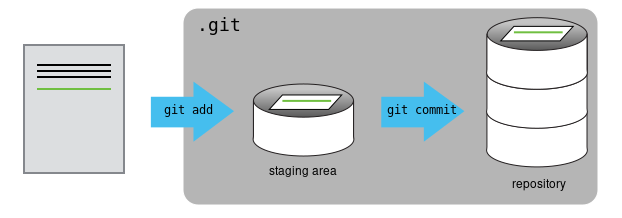
\includegraphics{D:/Users/hayde/Documents/R_sites/Computo_Cientifico/img/git-staging-area.png}
\caption{Software Carpentry - Version Control with Git}
\end{figure}

\textbf{Ejercicio:} Añadamos una tercera línea al archivo y verifiquemos las diferencias en los archivos, después añadamoslo al área de preparación y revicemos las diferencias. ¿Qué sucede?

\begin{Shaded}
\begin{Highlighting}[]
\ExtensionTok{$}\NormalTok{ nano prueba.txt}
\ExtensionTok{$}\NormalTok{ git diff}
\ExtensionTok{$}\NormalTok{ git add prueba.txt}
\ExtensionTok{$}\NormalTok{ git diff}
\end{Highlighting}
\end{Shaded}

Al añadirlo al área de preparación lo estamos añadiendo permanentemente, entonces no hay ninguna diferencia. Si queremos las diferencias con lo último a lo que se le hizo commit podemos hacer lo siguiente:

\begin{Shaded}
\begin{Highlighting}[]
\ExtensionTok{$}\NormalTok{ git diff }\AttributeTok{{-}{-}staged}
\end{Highlighting}
\end{Shaded}

Ahora hagamos el commit.

\begin{Shaded}
\begin{Highlighting}[]
\ExtensionTok{$}\NormalTok{ git commit }\AttributeTok{{-}m} \StringTok{"Tercera línea para probar que pasa cuando se añade al área de preparación"}
\end{Highlighting}
\end{Shaded}

Si revisamos el historial, veremos ahora 3 commit diferentes:

\begin{Shaded}
\begin{Highlighting}[]
\ExtensionTok{$}\NormalTok{ git log}
\end{Highlighting}
\end{Shaded}

Cuando el historial es muy grande no nos va a mostrar todo el historial nuestra terminal, para ir avanzando debemos presionar Spacebar y para salir la letra Q. Al presionar / se puede buscar alguna palabra en los mensajes de los commits. Para limitar la cantidad de información que nos regresa \texttt{log} podemos especificar con la opción \texttt{-n} la cantidad de commits desde el más reciente. Para ver por ejemplo el último utilizariamos lo siguiente:

\begin{Shaded}
\begin{Highlighting}[]
\ExtensionTok{$}\NormalTok{ git log }\AttributeTok{{-}1}
\end{Highlighting}
\end{Shaded}

Si queremos ver los mensajes en una sola línea usamos:

\begin{Shaded}
\begin{Highlighting}[]
\ExtensionTok{$}\NormalTok{ git log }\AttributeTok{{-}{-}oneline}
\end{Highlighting}
\end{Shaded}

Git no guarda información de directorios vacíos. Por ejemplo:

\begin{Shaded}
\begin{Highlighting}[]
\ExtensionTok{$}\NormalTok{ mkdir dic\_prueba}
\ExtensionTok{$}\NormalTok{ git status}
\ExtensionTok{$}\NormalTok{ git add dic\_prueba}
\ExtensionTok{$}\NormalTok{ git status}
\end{Highlighting}
\end{Shaded}

Si creamos un directorio con archivos, entonces si podemos añadir todos los archivos a la vez y si quedará el registro del directorio también.

\begin{Shaded}
\begin{Highlighting}[]
\ExtensionTok{$}\NormalTok{ git touch dic\_prueba/prueba1.txt dic\_prueba/prueba2.txt dic\_prueba/prueba3.txt}
\ExtensionTok{$}\NormalTok{ git status}
\ExtensionTok{$}\NormalTok{ git add dic\_prueba}
\ExtensionTok{$}\NormalTok{ git status}
\ExtensionTok{$}\NormalTok{ git commit }\AttributeTok{{-}m} \StringTok{"Ejemplo de como realizar un registro de directorios con archivos"}
\end{Highlighting}
\end{Shaded}

En algunas ocasiones verán directorios vacíos con un archivo \texttt{.gitkeep}, este archivo es solo para que podamos añadir el repo a Git.

\textbf{Ejercicio:} Crea un archivo \texttt{mi\_archivo.txt}, escribe algo en el y guárdalo en la ruta \texttt{Mi\_primer\_repo}. Añádelo a la historia de tu repo. ¿Cuáles son los pasos que debes realizar?

\textbf{Ejercicio:} Modifica el archivo \texttt{prueba.txt} añadiéndole una línea, ahora en el archivo \texttt{mi\_archivo.txt} agrega algo y guárdalo. ¿Cómo añadirías los dos archivos al staging área? Añádelos y realiza el commit correspondiente.

\textbf{Ejercicio:} Crea un repositorio llamado \texttt{bio}. Escribe en un archivo llamado \texttt{me.txt} tres líneas de tu biografía, has un commit con tus cambios. Modifica una línea y agrega una cuarta línea. Muestra las diferencias entre el archivo en el staging área y el actual.

\hypertarget{explorando-el-historial}{%
\section{Explorando el historial}\label{explorando-el-historial}}

A los commits nos podemos referir a ellos con sus identificadores. Al último commit también nos podemos referir como \texttt{HEAD}. Añadamos una línea más al archivo \texttt{prueba.txt}.

\begin{Shaded}
\begin{Highlighting}[]
\ExtensionTok{$}\NormalTok{ nano prueba.txt}
\ExtensionTok{$}\NormalTok{ cat prueba.txt}
\end{Highlighting}
\end{Shaded}

Ahora, para ver el último cambio con el último commit:

\begin{Shaded}
\begin{Highlighting}[]
\ExtensionTok{$}\NormalTok{ git diff HEAD prueba.txt}
\end{Highlighting}
\end{Shaded}

Si quitamos el HEAD de esa última instrucción veremos lo mismo. Pero si colocamos un \texttt{\textasciitilde{}numero} vamos a ver que nos estamos refiriendo al commit anterior número n.~

\begin{Shaded}
\begin{Highlighting}[]
\ExtensionTok{$}\NormalTok{ git diff HEAD\textasciitilde{}1 prueba.txt}
\end{Highlighting}
\end{Shaded}

Con \texttt{git\ show} vamos a ver los cambios con respecto a un commit anterior.

\begin{Shaded}
\begin{Highlighting}[]
\ExtensionTok{$}\NormalTok{ git show HEAD\textasciitilde{}1 prueba.txt}
\end{Highlighting}
\end{Shaded}

También podemos referirnos a los commit por su identificador de números y letras enorme o por los primeros 7 números o letras:

\begin{Shaded}
\begin{Highlighting}[]
\ExtensionTok{$}\NormalTok{ git diff 451b2ad469b96e13547e13dc0e718613acdc987c prueba.txt}
\ExtensionTok{$}\NormalTok{ git diff 451b2ad prueba.txt}
\end{Highlighting}
\end{Shaded}

Revisemos el estado:

\begin{Shaded}
\begin{Highlighting}[]
\ExtensionTok{$}\NormalTok{ git status}
\end{Highlighting}
\end{Shaded}

Con la siguiente instrucción podemos regresar las cosas a como estaban antes de hacer el último cambio.

\begin{Shaded}
\begin{Highlighting}[]
\ExtensionTok{$}\NormalTok{ git checkout HEAD prueba.txt}
\ExtensionTok{$}\NormalTok{ cat prueba.txt}
\end{Highlighting}
\end{Shaded}

O podríamos usar uno de los identificadores de commits:

\begin{Shaded}
\begin{Highlighting}[]
\ExtensionTok{$}\NormalTok{ git checkout 451b2ad prueba.txt}
\ExtensionTok{$}\NormalTok{ cat prueba.txt}
\ExtensionTok{$}\NormalTok{ git status}
\end{Highlighting}
\end{Shaded}

Y para regresarlo al último commit de nuevo:

\begin{Shaded}
\begin{Highlighting}[]
\ExtensionTok{$}\NormalTok{ git checkout HEAD prueba.txt}
\end{Highlighting}
\end{Shaded}

\begin{figure}
\centering
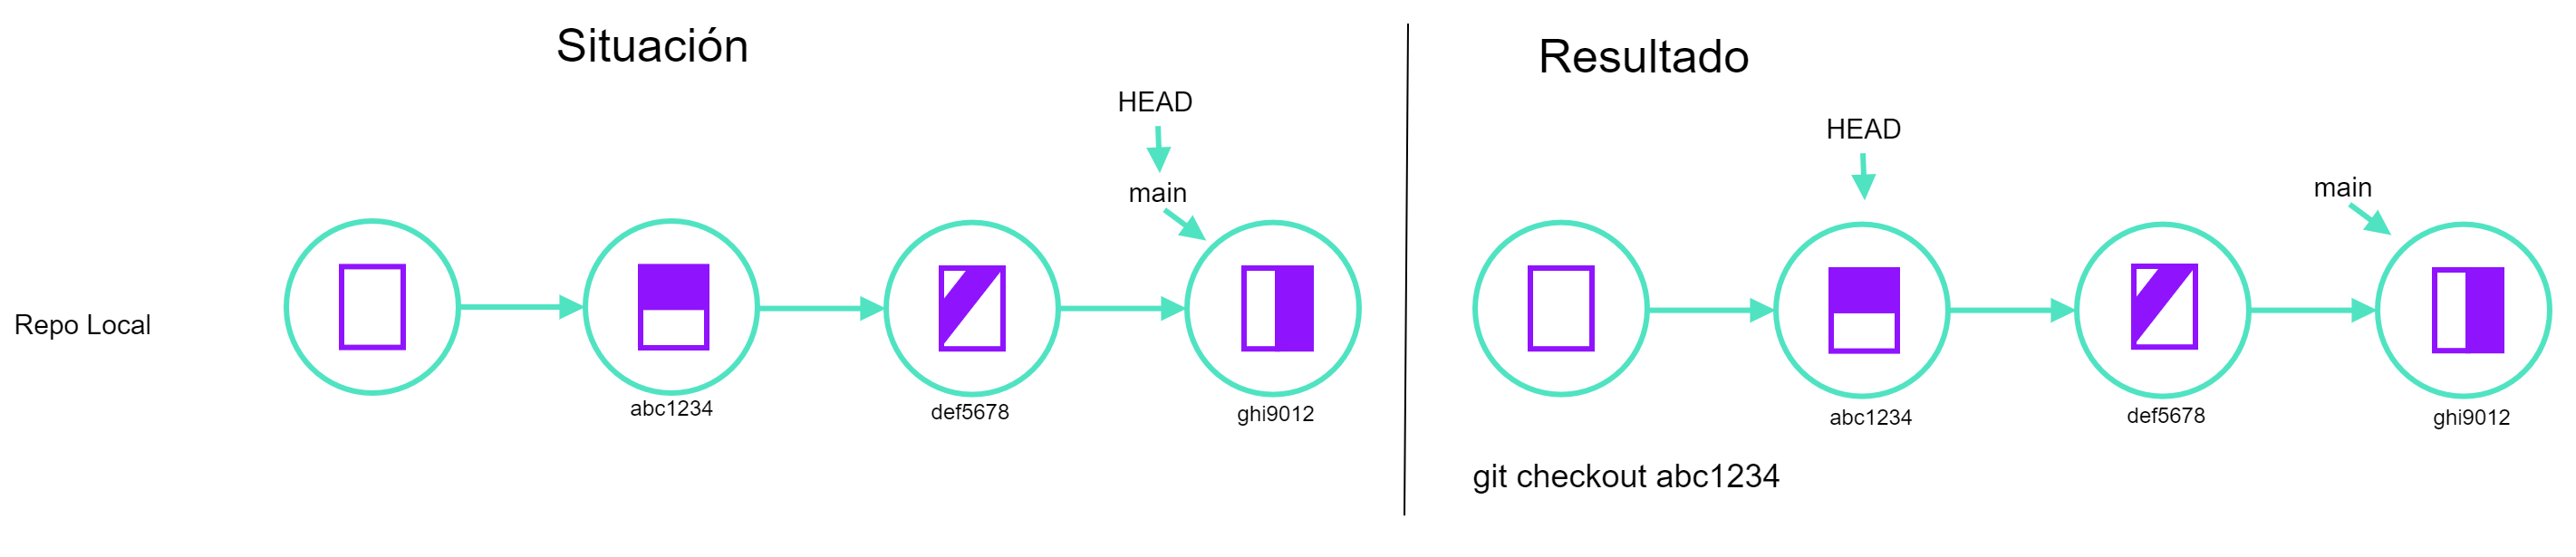
\includegraphics{D:/Users/hayde/Documents/R_sites/Computo_Cientifico/img/git-checkout.png}
\caption{\texttt{git\ checkout\ \textless{}ID\ commit\textgreater{}\ \textless{}archivo\textgreater{}}, basdo en ASSP}
\end{figure}

El comando \texttt{git\ checkout} revierte los archivos a alguna versión anterior siempre que no lo hayamos añadido al staging área. Para revertir un commit usamos la instrucción \texttt{git\ revert\ {[}ID\ commit{]}}. Supongamos que tenemos un error en el archivo \texttt{prueba.txt} y que ya hicimos commit y queremos revertir al último cambio. Los pasos que haríamos serían los siguientes:

\begin{enumerate}
\def\labelenumi{\arabic{enumi})}
\item
  \texttt{git\ log} para identificar el ID del commit.
\item
  Copiar el ID del commit
\item
  \texttt{git\ revert\ {[}ID\ del\ commit{]}} para revertir a ese cambio.
\item
  Teclear el nuevo mensaje de commit.
\item
  Guardar y cerrar
\end{enumerate}

\begin{figure}
\centering
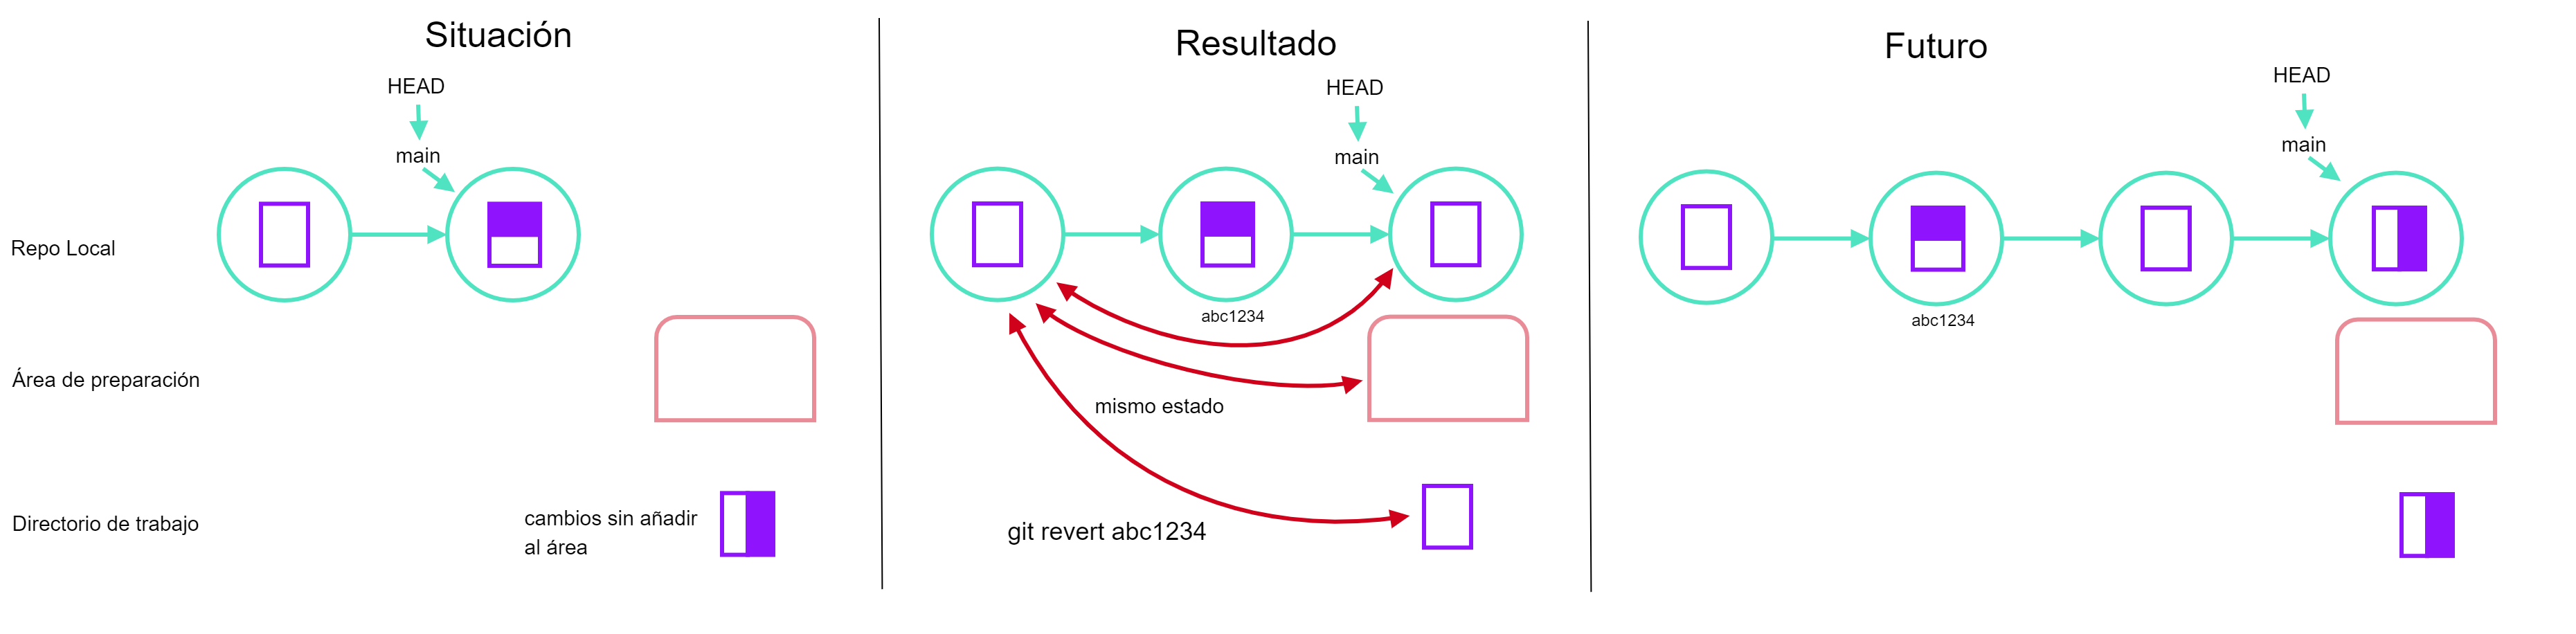
\includegraphics{D:/Users/hayde/Documents/R_sites/Computo_Cientifico/img/revert-commit.png}
\caption{\texttt{git\ revert\ \textless{}ID\ commit\textgreater{}}, basado en APP}
\end{figure}

Si ya añadimos los cambios al área de preparación, ya no podemos usar git checkout simplemente.

\textbf{Ejercicio:} Realiza las siguientes instrucciones:

\begin{enumerate}
\def\labelenumi{\arabic{enumi})}
\item
  Crea una carpeta llamada \texttt{learn\_revert}.
\item
  Muévete a la carpeta \texttt{learn\_revert}
\item
  Inicializa el repositorio.
\item
  Crea un archivo llamado \texttt{first.txt} y añade una línea de texto.
\item
  Agrégalo al área de preparación y realiza el primer commit.
\item
  Crea el archivo \texttt{wrong.txt} y agrega una línea de texto.
\item
  Agrégalo al área de preparación y realiza un commit.
\item
  Agrega una segunda línea de texto al archivo \texttt{first.txt}, guárdalo, agrégalo al área de preparación y realiza un commit.
\item
  Agrega una tercera línea de texto al archivo \texttt{first.txt}, guárdalo, agrégalo al área de preparación y realiza un commit.
\item
  Queremos deshacer el commit realizado cuando se añadió el archivo \texttt{wrong.txt}. Como este commit fue el segundo de donde no estamos, podemos usar \texttt{git\ revert\ HEAD\textasciitilde{}2} (o podemos usar \texttt{git\ log} y encontrar el ID de ese commit).
\end{enumerate}

¿Está el archivo \texttt{wrong.txt}? ¿Qué sucede con el historial de commits?

Otras opciones del historial del commit:

\begin{enumerate}
\def\labelenumi{\arabic{enumi})}
\tightlist
\item
  Para ver tanto las diferencias entre los archivos y los ID de los commits. Se puede colocar solo el nombre de un archivo y solo mostrara los commit que afectaban ese archivo o si no se coloca el nombre del archivo aplica sobre todo el historial de commits.
\end{enumerate}

\begin{Shaded}
\begin{Highlighting}[]
\ExtensionTok{$}\NormalTok{ git log }\AttributeTok{{-}{-}patch}\NormalTok{ prueba.txt}
\end{Highlighting}
\end{Shaded}

\begin{enumerate}
\def\labelenumi{\arabic{enumi})}
\setcounter{enumi}{1}
\tightlist
\item
  Para mostrar las descripciones detalladas de las modificaciones y archivos.
\end{enumerate}

\begin{Shaded}
\begin{Highlighting}[]
\ExtensionTok{$}\NormalTok{ git log }\AttributeTok{{-}p}
\end{Highlighting}
\end{Shaded}

\begin{enumerate}
\def\labelenumi{\arabic{enumi})}
\setcounter{enumi}{2}
\tightlist
\item
  Para mostrar los nombres de los archivos afectados en cada commit.
\end{enumerate}

\begin{Shaded}
\begin{Highlighting}[]
\ExtensionTok{$}\NormalTok{ git log }\AttributeTok{{-}{-}name{-}only}
\end{Highlighting}
\end{Shaded}

\begin{enumerate}
\def\labelenumi{\arabic{enumi})}
\setcounter{enumi}{3}
\tightlist
\item
  Para mostrar los archivos afectados en cada commit con la leyenda de si fueron modificados (M) o añadidos (A) o eliminados.
\end{enumerate}

\begin{Shaded}
\begin{Highlighting}[]
\ExtensionTok{$}\NormalTok{ git log }\AttributeTok{{-}{-}name{-}status}
\end{Highlighting}
\end{Shaded}

Consultar el siguiente \href{https://git-scm.com/book/es/v2/Fundamentos-de-Git-Ver-el-Historial-de-Confirmaciones}{link} para ver más opciones y ejemplos.

\hypertarget{restore-y-reset}{%
\section{Restore y reset}\label{restore-y-reset}}

Otra forma de deshacer cambios es con \texttt{restore} y \texttt{reset}. Usualmente deshacer cambios se requiere para deshacer:

\begin{itemize}
\item
  Cambios antes de mandarlos al área de preparación.
\item
  Cambios que ya se mandaron al área de preparación.
\item
  Commits
\end{itemize}

Supongamos que hicimos un cambio en el archivo de prueba y lo guardamos y después decidimos que ya no queremos ese cambio, entonces usamos la opción:

\begin{Shaded}
\begin{Highlighting}[]
\ExtensionTok{$}\NormalTok{ git restore prueba.txt}
\end{Highlighting}
\end{Shaded}

Esto nos regresará a la versión del archivo del último commit. Esto no se puede deshacer, una vez echo esto no hay forma de recuperar los cambios que se habían realizado.

\begin{figure}
\centering
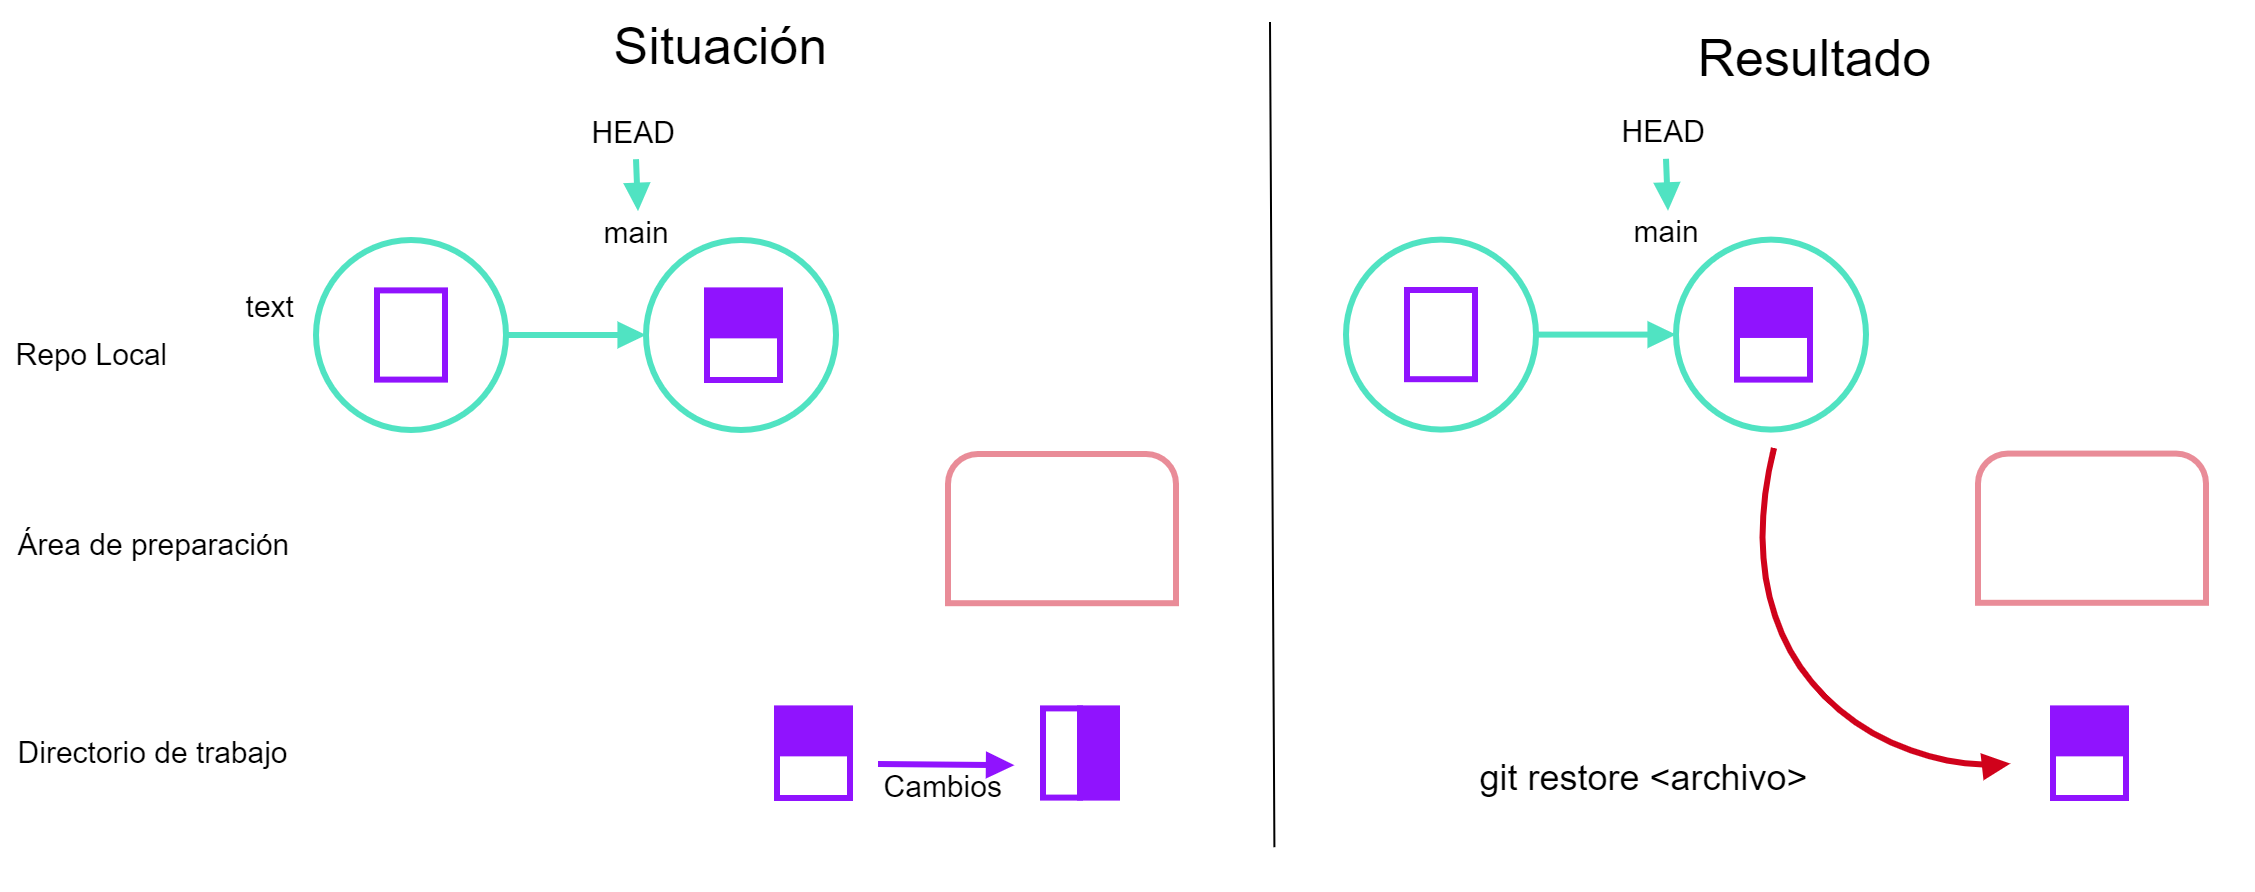
\includegraphics{D:/Users/hayde/Documents/R_sites/Computo_Cientifico/img/restore-archivo.png}
\caption{\texttt{git\ restore\ \textless{}archivo\textgreater{}}, basado en ASSP}
\end{figure}

Ahora, supongamos que hicimos un cambio y lo mandamos al área de preparación, entonces para sacarlo de esa área usamos:

\begin{Shaded}
\begin{Highlighting}[]
\ExtensionTok{$}\NormalTok{ git restore }\AttributeTok{{-}{-}staged}\NormalTok{ prueba.txt}
\end{Highlighting}
\end{Shaded}

\begin{figure}
\centering
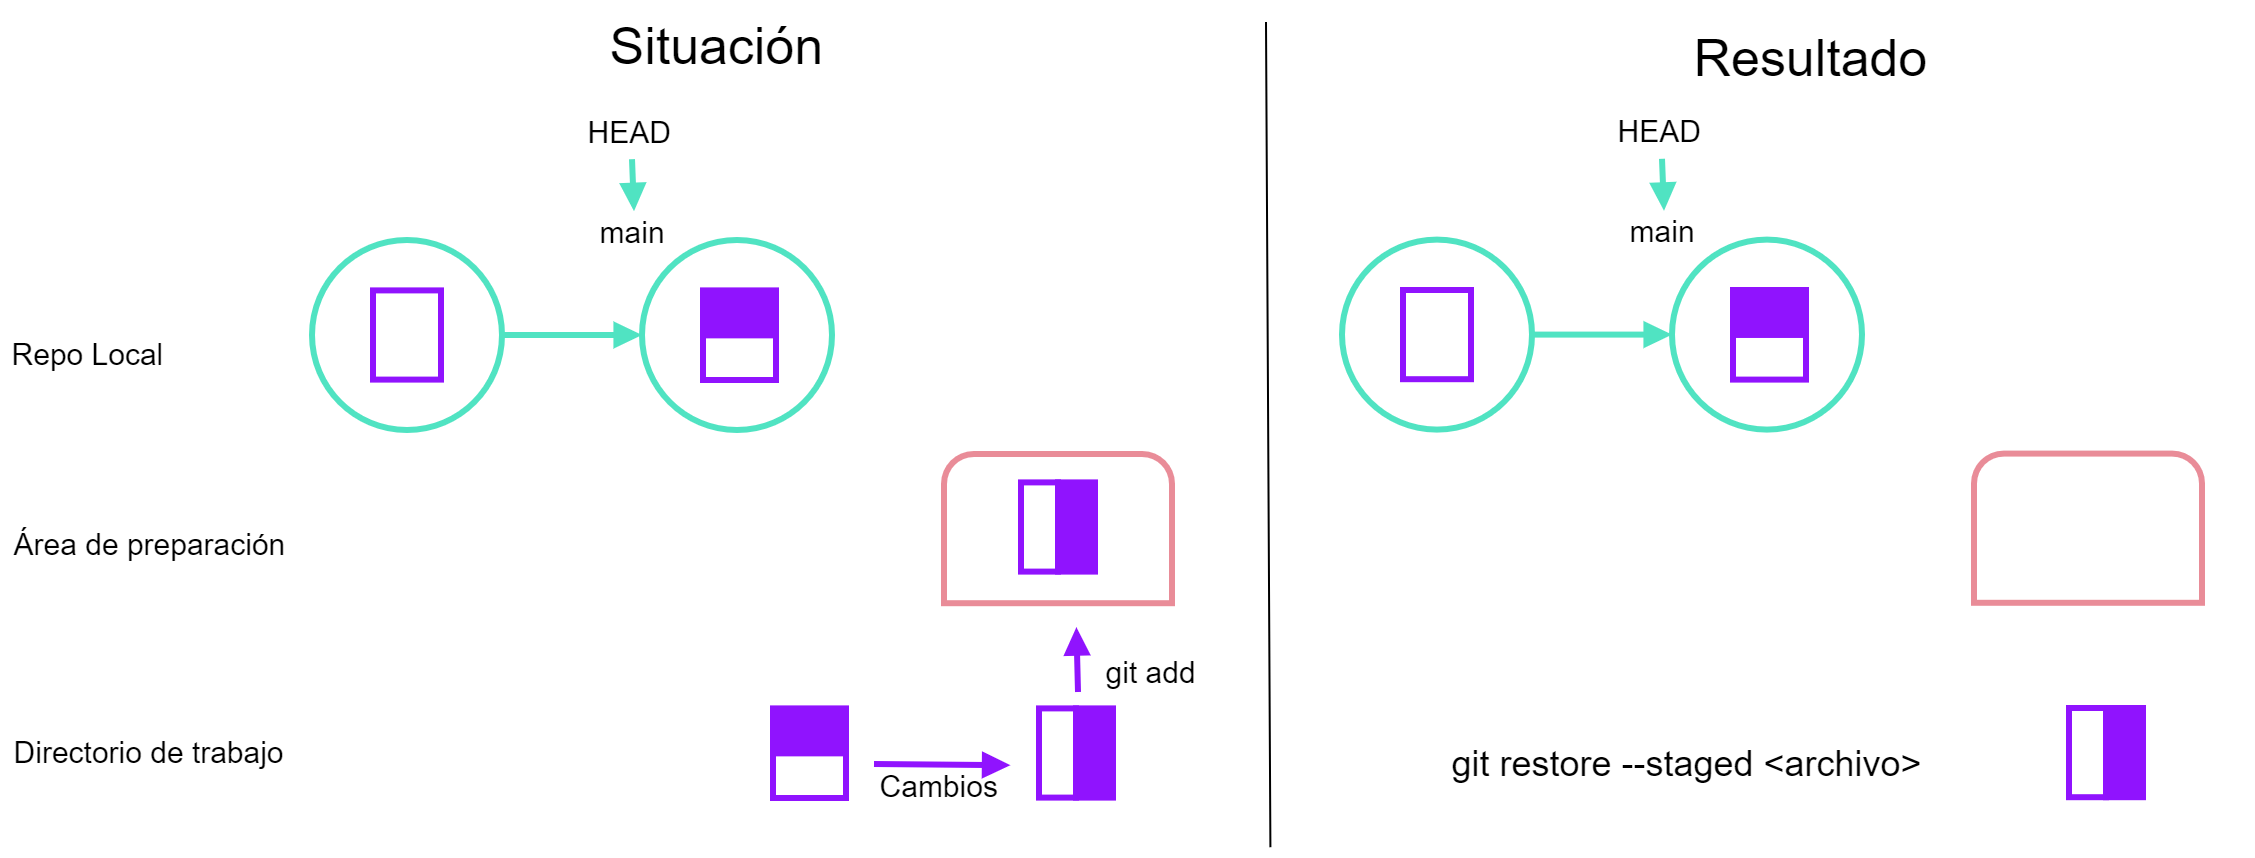
\includegraphics{D:/Users/hayde/Documents/R_sites/Computo_Cientifico/img/restore-staged.png}
\caption{\texttt{git\ restore\ -\/-staged\ \textless{}archivo\textgreater{}}, basado en ASSP}
\end{figure}

También se pueden restaurar todos los archivos de un proyecto con:

\begin{Shaded}
\begin{Highlighting}[]
\ExtensionTok{$}\NormalTok{ git restore .}
\end{Highlighting}
\end{Shaded}

Para restaurar a un commit anterior usamos el identificador del commit, por ejemplo:

\begin{Shaded}
\begin{Highlighting}[]
\ExtensionTok{$}\NormalTok{ git restore }\AttributeTok{{-}{-}source}\NormalTok{ d3a9d6d prueba.txt}
\end{Highlighting}
\end{Shaded}

Si ahora revisamos el estado del proyecto veremos que si hay cambios.

Agreguemos una línea al archivo \texttt{prueba.txt} y añadamos el cambio al área de preparación. Usen \texttt{git\ checkout} para ver si podemos revertir el cambio. Veamos que nos dice el estado \texttt{git\ status}. Si usamos \texttt{git\ checkout\ -\/-\ prueba.txt} ya no veremos errores pero tampoco se restaurará el archivo.

Para hacerlo debemos usar \texttt{reset}:

\begin{Shaded}
\begin{Highlighting}[]
\ExtensionTok{$}\NormalTok{ git reset HEAD prueba.txt}
\end{Highlighting}
\end{Shaded}

Y si usamos ahora:

\begin{Shaded}
\begin{Highlighting}[]
\ExtensionTok{$}\NormalTok{ git status}
\end{Highlighting}
\end{Shaded}

Nos indica que ya podemos realizar la modificación con checkout:

\begin{Shaded}
\begin{Highlighting}[]
\ExtensionTok{$}\NormalTok{ git checkout }\AttributeTok{{-}{-}}\NormalTok{ prueba.txt}
\ExtensionTok{$}\NormalTok{ git status}
\end{Highlighting}
\end{Shaded}

Con \texttt{reset} tenemos tres posibles situaciones.

\begin{itemize}
\tightlist
\item
  Situación 1: \texttt{reset\ -\/-soft\ HEAD\textasciitilde{}1}: si realizamos un cambio en nuestro archivo y lo añadimos al área de preparación, al realizar el \texttt{reset\ soft} al commit \texttt{HEAD\textasciitilde{}1} lo que estamos haciendo es como regresar a un commit anterior pero sin perder los cambios que ya tenemos en el área de preparación, entonces lo que va a resultar es que nuestro historial va a cambiar de un commit anterior hasta el cambio que tenemos ahora. Con \texttt{git\ status} vemos que no cambio nuestra área de preparación y después con \texttt{git\ log} podemos ver el cambio en el historial de commits.
\end{itemize}

\begin{figure}
\centering
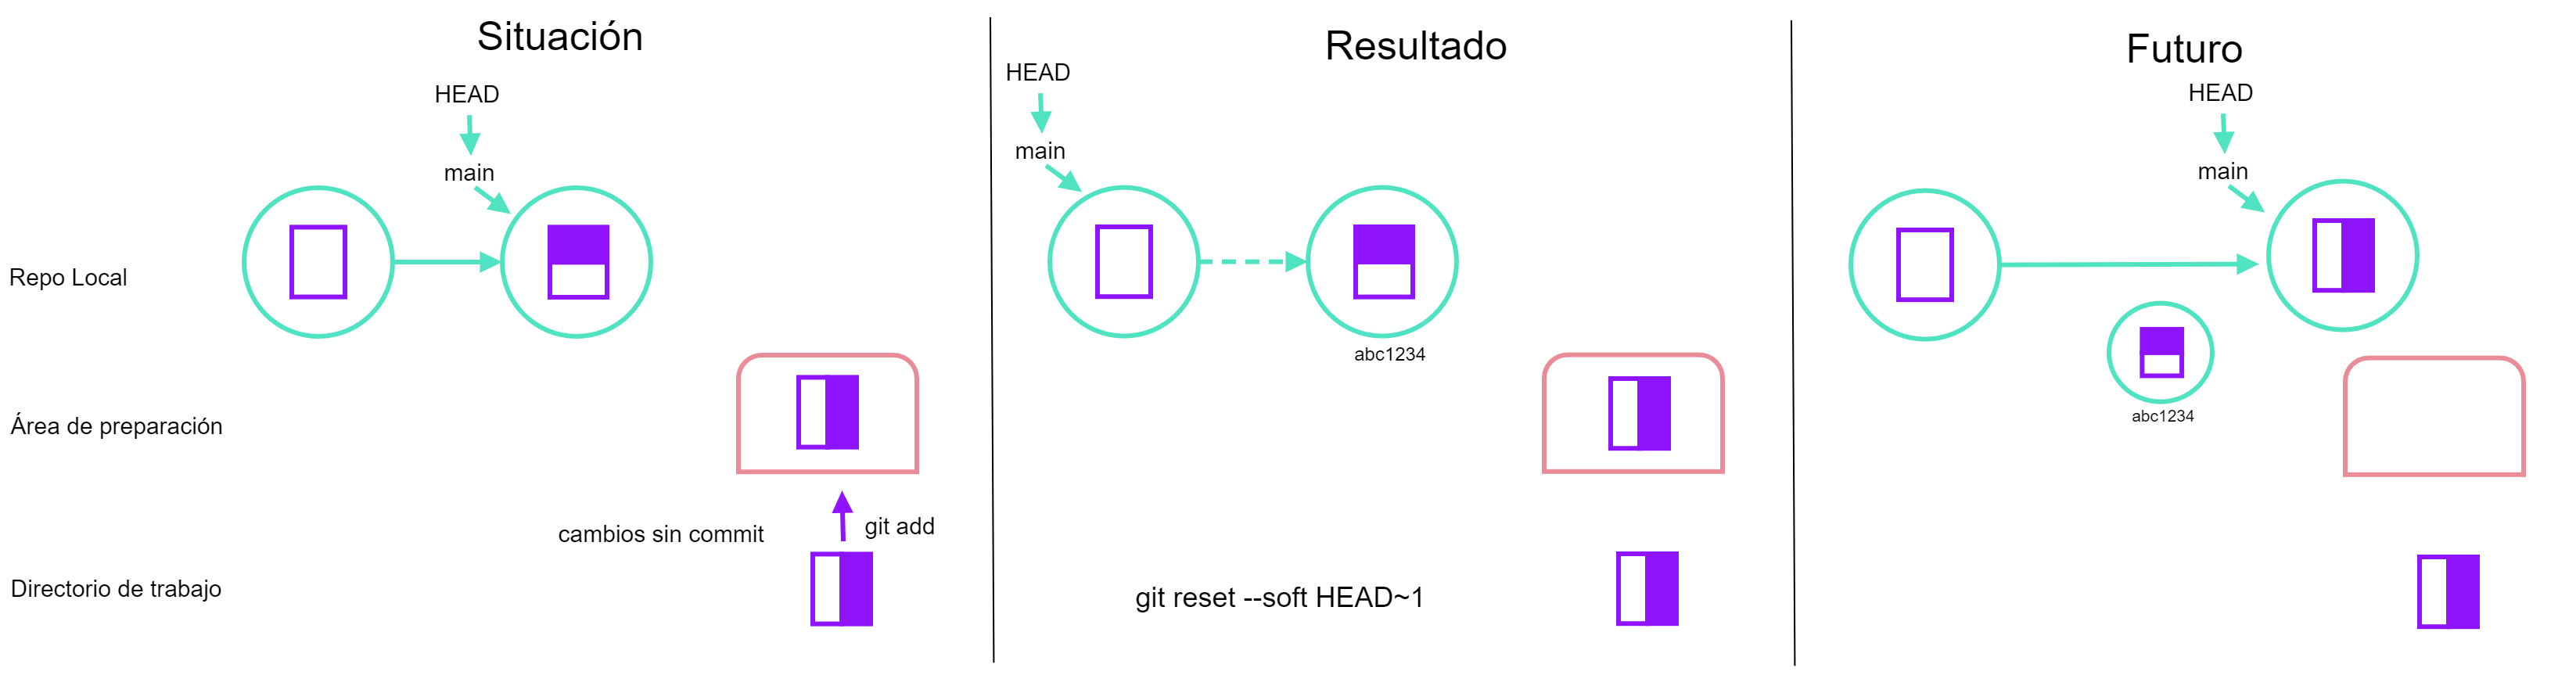
\includegraphics{D:/Users/hayde/Documents/R_sites/Computo_Cientifico/img/reset-soft.png}
\caption{\texttt{git\ reset\ -\/-soft\ HEAD\textasciitilde{}1}, basado en ASSP}
\end{figure}

\begin{itemize}
\tightlist
\item
  Situación 2: \texttt{reset\ -\/-mixed\ HEAD\textasciitilde{}1}: si realizamos un cambio en nuestro archivo y lo añadimos al área de preparación, al realizar el \texttt{reset\ mixed} al commit \texttt{HEAD\textasciitilde{}1} lo que estamos haciendo es como regresar nuestra área de preparación a como estaba antes de ese commit, no perdemos el cambio realizado en el archivo pero nuestro historial cambiará, pasará del commit anterior hasta el próximo commit que realicemos. Con \texttt{git\ status} vemos que nuestra área de preparación si cambio y con \texttt{git\ log} vemos que nuestro último commit desapareció.
\end{itemize}

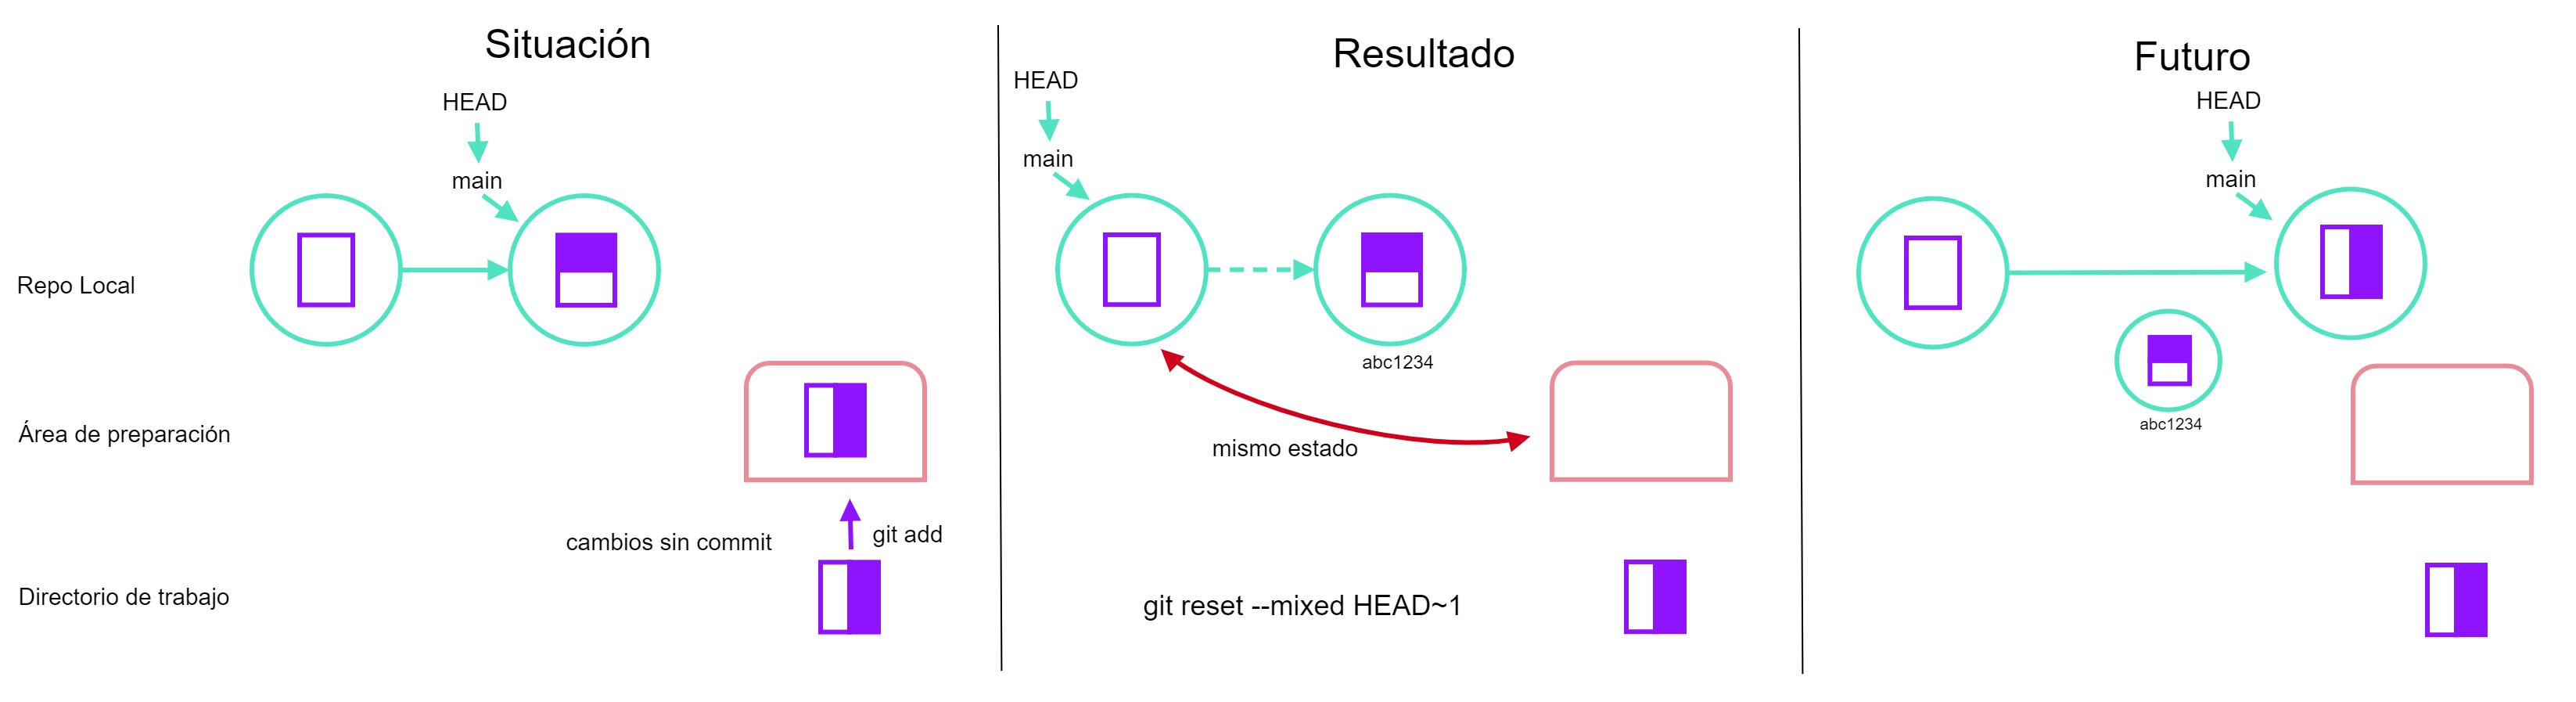
\includegraphics{D:/Users/hayde/Documents/R_sites/Computo_Cientifico/img/reset-mixed.png}
- Situación 3: \texttt{reset\ -\/-hard\ HEAD\textasciitilde{}1}: si realizamos un cambio en nuestro archivo y lo añadimos al área de preparación, al realizar el \texttt{reset\ hard} al commit \texttt{HEAD\textasciitilde{}1} lo que estamos haciendo es como regresar a un commit anterior pero perdiendo los cambios que ya tenemos en el área de preparación y en nuestro archivo actual, entonces lo que va a resultar es que estaríamos regresando hasta el commit anterior todo nuestro historial y a partir de ahí comenzarían nuestros cambios.

\begin{figure}
\centering
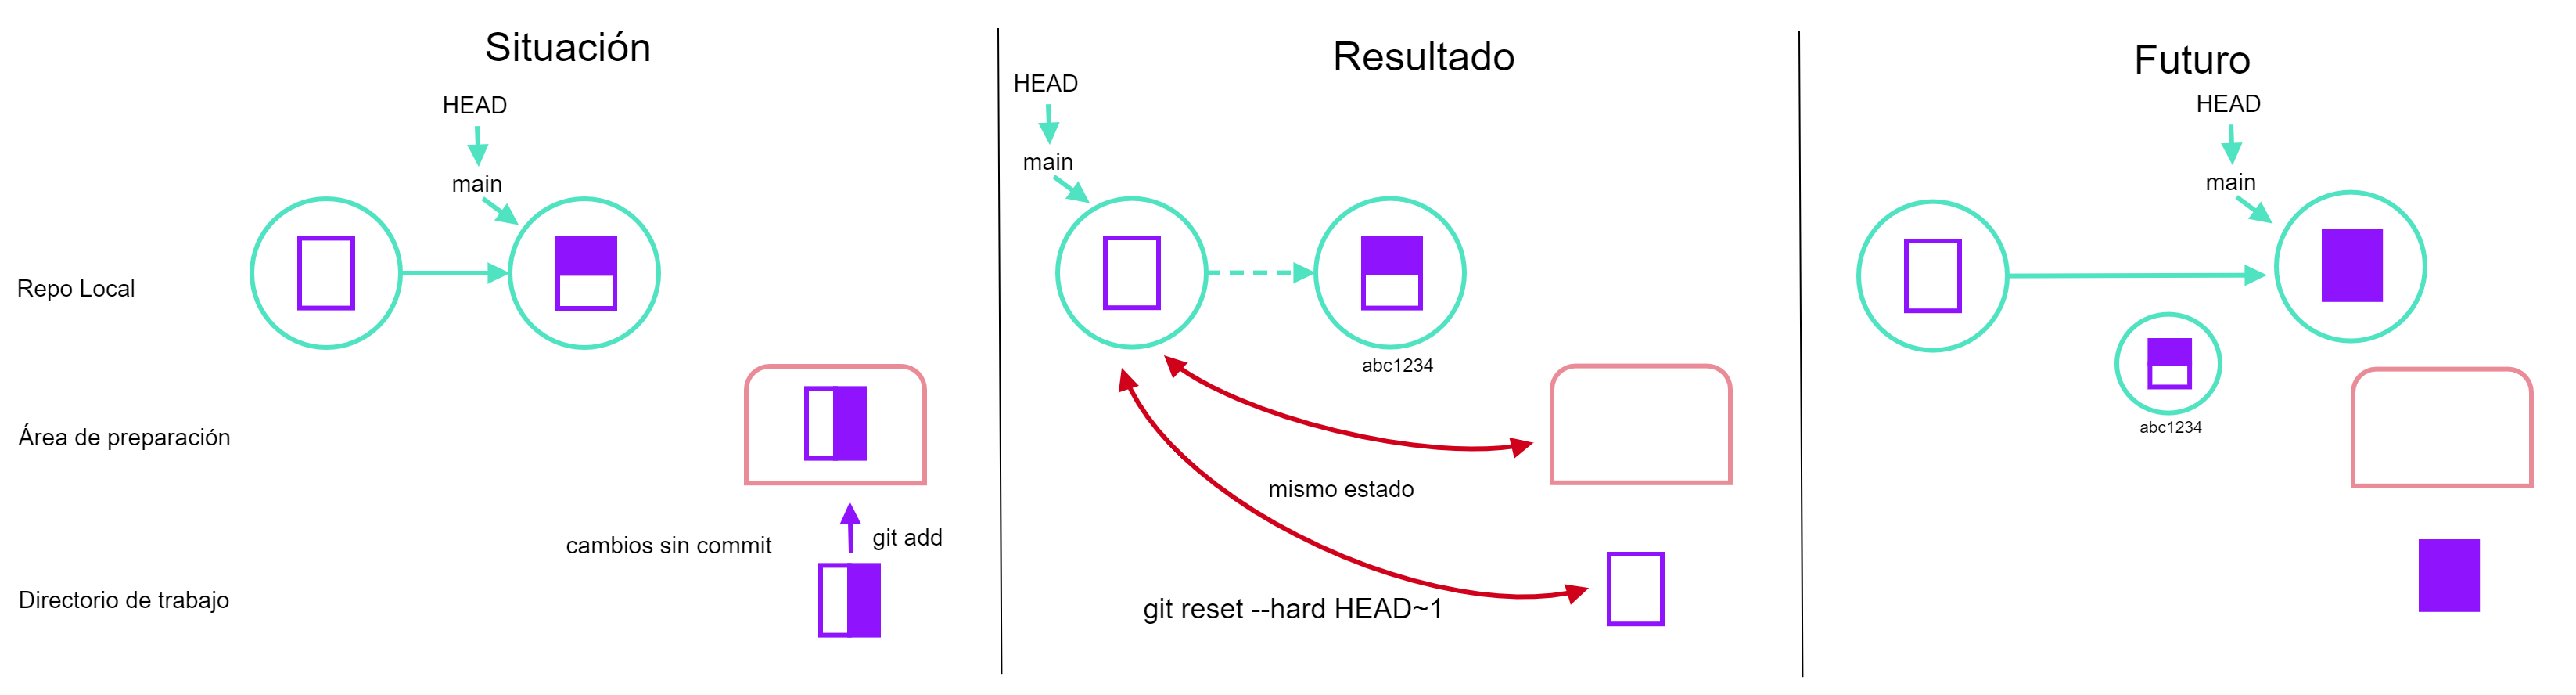
\includegraphics{D:/Users/hayde/Documents/R_sites/Computo_Cientifico/img/reset-hard.png}
\caption{\texttt{git\ reset\ -\/-hard\ HEAD\textasciitilde{}1}, basado en ASSP}
\end{figure}

\hypertarget{ignorar-archivoscarpetas}{%
\section{Ignorar archivos/carpetas}\label{ignorar-archivoscarpetas}}

Es muy usual tener un archivo llamado \texttt{.gitignore} donde se pueden colocar los nombres de archivos o carpetas que no queremos llevar registro.

Creemos unos archivos de prueba.

\begin{Shaded}
\begin{Highlighting}[]
\ExtensionTok{$}\NormalTok{ cd Mi\_primer\_repo}
\ExtensionTok{$}\NormalTok{ mkdir resultados}
\ExtensionTok{$}\NormalTok{ touch a.csv b.csv c.csv resultados/a.out resultados/b.out}
\end{Highlighting}
\end{Shaded}

Si preguntamos el estado veremos los cambios no registrados en el historial.

\begin{Shaded}
\begin{Highlighting}[]
\ExtensionTok{$}\NormalTok{ git status}
\end{Highlighting}
\end{Shaded}

Estos archivos por el momento no nos sirven de nada y guardarlos o registrarlos sería una perdida de tiempo/espacio. Para ignorarlos, creamos el archivo \texttt{.gitigno} y añadimos los nombres a ese archivo:

\begin{Shaded}
\begin{Highlighting}[]
\ExtensionTok{$}\NormalTok{ nano .gitignore}
\end{Highlighting}
\end{Shaded}

\begin{Shaded}
\begin{Highlighting}[]
\ExtensionTok{*.csv}
\ExtensionTok{resultados/}
\end{Highlighting}
\end{Shaded}

\begin{Shaded}
\begin{Highlighting}[]
\ExtensionTok{$}\NormalTok{ cat .gitignore}
\end{Highlighting}
\end{Shaded}

Estos patrones le están diciendo a Git que ignore todos los archivos \texttt{.csv} y todo lo que hay en la carpeta \texttt{resultados}, si después añadimos algo a la carpeta lo seguirá ignorando. Y si alguno de esos archivos ya se le dijo a Git que llevará su registro lo seguirá registrando.

\begin{Shaded}
\begin{Highlighting}[]
\ExtensionTok{$}\NormalTok{ git status}
\end{Highlighting}
\end{Shaded}

Si nos fijamos, el único documento que ahora nos menciona \texttt{Git} es el archivo \texttt{.gitignore}. Lo que nos falta es añadirlo y hacer el commit.

\begin{Shaded}
\begin{Highlighting}[]
\ExtensionTok{$}\NormalTok{ git add .gitignore}
\ExtensionTok{$}\NormalTok{ git commit }\AttributeTok{{-}m} \StringTok{"Creamos el archivo gitignore e ignoramos todo lo que hay en resultados y archivos csv"}
\ExtensionTok{$}\NormalTok{ git status}
\end{Highlighting}
\end{Shaded}

El archivo \texttt{.gitignore} nos ayuda a no cometer el error de accidentalmente tratar de registrar y rastrear algo que se le dijo que no lo hiciera.

\begin{Shaded}
\begin{Highlighting}[]
\ExtensionTok{$}\NormalTok{ git add a.csv}
\end{Highlighting}
\end{Shaded}

Si realmente queremos agregarlo, tendríamos que usar la opción \texttt{-f}:

\begin{Shaded}
\begin{Highlighting}[]
\ExtensionTok{$}\NormalTok{ git add }\AttributeTok{{-}f}\NormalTok{ a.csv}
\end{Highlighting}
\end{Shaded}

Para ver el estado de los archivos ignorados usamos la siguiente instrucción:

\begin{Shaded}
\begin{Highlighting}[]
\ExtensionTok{$}\NormalTok{ git status }\AttributeTok{{-}{-}ignored}
\end{Highlighting}
\end{Shaded}

\textbf{Ejercicio:} Supongamos que tenemos las siguientes subcarpetas:

\begin{Shaded}
\begin{Highlighting}[]
\ExtensionTok{resultados/plots}
\ExtensionTok{resultados/datos}
\end{Highlighting}
\end{Shaded}

¿Qué tenemos que hacer si queremos ignorar solamente lo que hay en \texttt{datos} y no lo que hay en \texttt{plots}?

Para ignorar por ejemplo todos los archivos que terminan en \texttt{.csv} excepto uno en específico (\texttt{b.csv}) podemos indicarlo en el archivo \texttt{.gitignore} como:

\begin{Shaded}
\begin{Highlighting}[]
\ExtensionTok{*.csv}  \CommentTok{\# ignoramos todos los csv}
\ExtensionTok{!b.csv} \CommentTok{\# exepto el que se llama b.csv}
\end{Highlighting}
\end{Shaded}

\textbf{Ejercicio:} Supongamos ahora que tenemos la siguiente estructura de carpetas:

\begin{Shaded}
\begin{Highlighting}[]
\ExtensionTok{resultados/plots}
\ExtensionTok{resultados/datos}
\ExtensionTok{resultados/img}
\ExtensionTok{resultados/analisis}
\end{Highlighting}
\end{Shaded}

Y que queremos ignorar todo excepto lo que hay en datos. ¿Cómo lo harían?

\textbf{Ejemplo:} Supongamos que tenemos la siguiente estructura de archivos:

\begin{Shaded}
\begin{Highlighting}[]
\ExtensionTok{resultados/rdatos/a.csv}
\ExtensionTok{resultados/rdatos/b.csv}
\ExtensionTok{resultados/rdatos/c.csv}
\ExtensionTok{resultados/rdatos/info.txt}
\end{Highlighting}
\end{Shaded}

¿Cómo le indicas a Git que ignore todos los \texttt{csv} de la carpeta \texttt{rdatos} menos el que se llama \texttt{info.txt}?

\textbf{Ejercicio:} Supongamos que tenemos la siguiente estructura de datos:

\begin{Shaded}
\begin{Highlighting}[]
\ExtensionTok{resultados/a.csv}
\ExtensionTok{resultados/analisis1/b.csv}
\ExtensionTok{resultados/analisis2/c.csv}
\ExtensionTok{resultados/analisis2/sub\_1/d.csv}
\end{Highlighting}
\end{Shaded}

¿Cómo le indicamos a Git que ignore todos los archivos \texttt{.csv} sin indicar manualmente todos los directorios?

\textbf{Ejercicio:} Si en el archivo \texttt{.gitignore} escribimos lo siguiente, ¿qué está ignorando?

\begin{Shaded}
\begin{Highlighting}[]
\ExtensionTok{*.csv}
\ExtensionTok{!*.csv}
\end{Highlighting}
\end{Shaded}

\hypertarget{github}{%
\section{Github}\label{github}}

El valor del control de versiones se hace evidente al comenzar a colaborar con otros. Contamos con la mayor parte de las herramientas necesarias para ello; lo único que resta es transferir cambios de un repositorio a otro.

Sistemas como Git posibilitan el traslado de trabajo entre cualquier par de repositorios. No obstante, en la práctica, resulta más conveniente utilizar una copia como punto central y mantenerla en la web en lugar de en la computadora portátil de alguien.

Vamos a comenzar por crear un repositorio remoto, pero para eso necesitamos configurar nuestra cuenta de Github también.

\hypertarget{paso-1-crear-un-repositorio-remoto}{%
\subsection{Paso 1: Crear un repositorio remoto}\label{paso-1-crear-un-repositorio-remoto}}

Lo primero que vamos a hacer es crear un repositorio remoto. Entra a tu cuenta de Github y dale click en Nuevo.

\begin{figure}
\centering

\includegraphics{D:/Users/hayde/Documents/R_sites/Computo_Cientifico/img/github_1.png}
\caption{Crear repositorio nuevo}
\end{figure}

Ponle de nombre \texttt{Mi\_primer\_repo} (o el nombre que hayas usado en las secciones anteriores). Deja marcada la opción de público y no añadas un README ni una licencia.

\begin{figure}
\centering
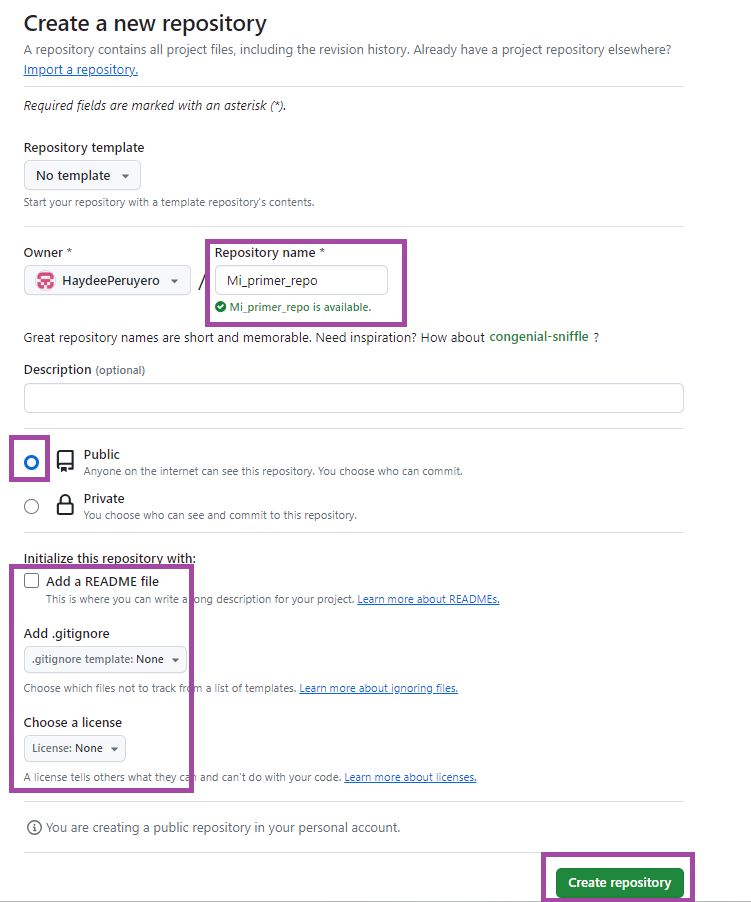
\includegraphics{D:/Users/hayde/Documents/R_sites/Computo_Cientifico/img/github_2.png}
\caption{Crear repositorio vacío}
\end{figure}

Al darle click en crear repositorio, la página nos mostrará la siguiente información que es la que usaremos para configurar nuestro local con el remoto.

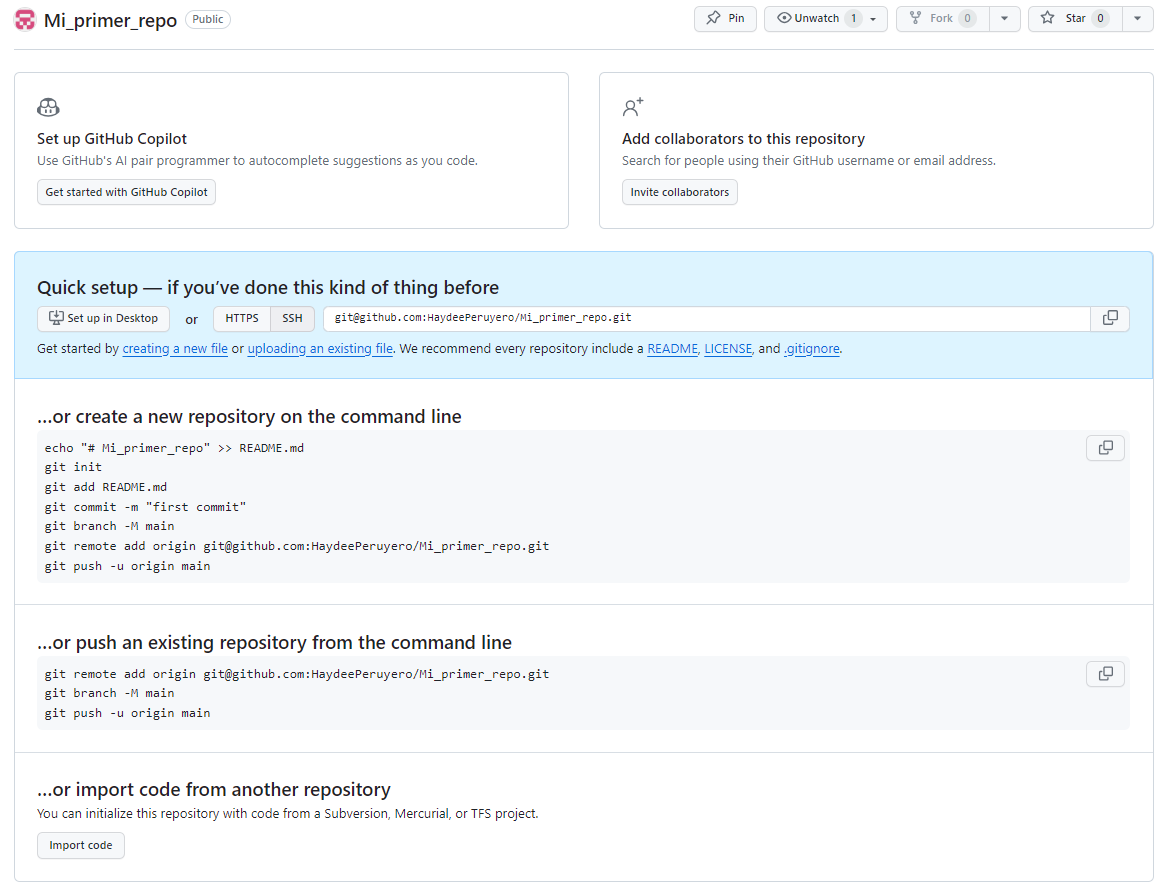
\includegraphics{D:/Users/hayde/Documents/R_sites/Computo_Cientifico/img/github_3.png}
Lo que acabamos de hacer es como si en nuestra terminal hubiéramos realizado lo siguiente:

\begin{Shaded}
\begin{Highlighting}[]
\ExtensionTok{$}\NormalTok{ mkdir Mi\_primer\_repo}
\ExtensionTok{$}\NormalTok{ cd Mi\_primer\_repo}
\ExtensionTok{$}\NormalTok{ git init}
\end{Highlighting}
\end{Shaded}

\hypertarget{paso-2-conectar-local-a-remoto}{%
\subsection{Paso 2: Conectar local a remoto}\label{paso-2-conectar-local-a-remoto}}

La página principal del repositorio remoto muestra una serie de información que necesitamos usar para conectar el repositorio remoto en Github con el repositorio local de nuestra computadora. Vamos a usar el protocolo de conexión SSH, da click en donde dice SSH y a continuación en el icono de copiar.

\begin{figure}
\centering
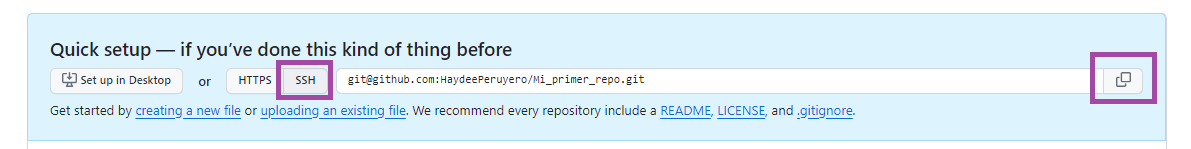
\includegraphics{D:/Users/hayde/Documents/R_sites/Computo_Cientifico/img/github_4.png}
\caption{SSH link para clonar el repositorio}
\end{figure}

Ahora, dentro de nuestra carpeta del repositorio local, abrir una terminal y correr lo siguiente:

\begin{Shaded}
\begin{Highlighting}[]
\ExtensionTok{$}\NormalTok{ git remote add origin git@github.com:User/Mi\_primer\_repo.git}
\end{Highlighting}
\end{Shaded}

Para revisar que si se haya realizado correctamente procedemos a usar lo siguiente:

\begin{Shaded}
\begin{Highlighting}[]
\ExtensionTok{$}\NormalTok{ git remote }\AttributeTok{{-}v}
\end{Highlighting}
\end{Shaded}

\hypertarget{paso-3-conexiuxf3n-mediante-ssh}{%
\subsection{Paso 3: Conexión mediante SSH}\label{paso-3-conexiuxf3n-mediante-ssh}}

Primero verificamos si ya tenemos algún par de llaves:

\begin{Shaded}
\begin{Highlighting}[]
\ExtensionTok{$}\NormalTok{ ls }\AttributeTok{{-}al}\NormalTok{ \textasciitilde{}/.ssh}
\end{Highlighting}
\end{Shaded}

Si ya tienen algún par de llaves configuradas las van a ver listadas, si no tiene ninguna les saldrá una leyenda como la siguiente:

\begin{Shaded}
\begin{Highlighting}[]
\NormalTok{ls: cannot access \textquotesingle{}/c/Users/User/.ssh\textquotesingle{}: No such file or directory}
\end{Highlighting}
\end{Shaded}

\hypertarget{paso-3.1-crear-un-par-de-llaves-ssh}{%
\subsubsection{Paso 3.1: Crear un par de llaves SSH}\label{paso-3.1-crear-un-par-de-llaves-ssh}}

Para crear el par de llaves usamos el siguiente comando, la opción \texttt{-t} se refiere al tipo de algoritmo usado y la opción \texttt{-C} indica un comentario para la llave, en este caso el comentario es nuestro correo.

\begin{Shaded}
\begin{Highlighting}[]
\ExtensionTok{$}\NormalTok{ ssh{-}keygen }\AttributeTok{{-}t}\NormalTok{ ed25519 }\AttributeTok{{-}C} \StringTok{"email@dominio.com"}
\end{Highlighting}
\end{Shaded}

Si tu sistema operativo no lo permite, usa \texttt{ssh-keygen\ -t\ rsa\ -b\ 4096\ -C\ "your\_email@example.com"}.

Como queremos usar el archivo default, solo damos Enter. Ahora nos pedirá una contraseña, tecleala, no vas a ver nada en la pantalla. Una vez creada verás en pantalla algo como lo siguiente:

\begin{Shaded}
\begin{Highlighting}[]
\ExtensionTok{Your}\NormalTok{ identification has been saved in /c/Users/user/.ssh/id\_ed25519}
\ExtensionTok{Your}\NormalTok{ public key has been saved in /c/Users/user/.ssh/id\_ed25519.pub}
\ExtensionTok{The}\NormalTok{ key fingerprint is:}
\ExtensionTok{SHA256:SMSPIStNyA10KPxuYu94KpZg9AYjgt9g46A4kFy3g1o}\NormalTok{ user@domain}
\ExtensionTok{The}\NormalTok{ keys randomart image is:}
\ExtensionTok{+{-}{-}[ED25519}\NormalTok{ 256]{-}{-}+}
\KeywordTok{|}\ExtensionTok{\^{}B==}\NormalTok{ o.          }\KeywordTok{|}
\KeywordTok{|}\ExtensionTok{\%*=} \PreprocessorTok{*}\NormalTok{.+          }\KeywordTok{|}
\KeywordTok{|}\ExtensionTok{+=.E}\NormalTok{ =.+         }\KeywordTok{|}
\KeywordTok{|} \BuiltInTok{.}\NormalTok{=.+.o..        }\KeywordTok{|}
\KeywordTok{|}\ExtensionTok{...}\NormalTok{   . S        }\KeywordTok{|}
\KeywordTok{|}\BuiltInTok{.}\NormalTok{+ o             }\KeywordTok{|}
\KeywordTok{|}\ExtensionTok{+}\NormalTok{ =              }\KeywordTok{|}
\KeywordTok{|}\ExtensionTok{.o.o}             \KeywordTok{|}
\KeywordTok{|}\ExtensionTok{oo+.}             \KeywordTok{|}
\ExtensionTok{+{-}{-}{-}{-}[SHA256]{-}{-}{-}{-}{-}+}
\end{Highlighting}
\end{Shaded}

Lo que dice \texttt{identification} ser refiere a la llave privada la cual no debes compartir nunca y la cadena de caracteres que dice \texttt{fingerprint} se refiere a parte de tu llave pública.

Si repetimos el comando siguiente, verán ahora ya sus dos claves pública y privada.

\begin{Shaded}
\begin{Highlighting}[]
\ExtensionTok{$}\NormalTok{ ls }\AttributeTok{{-}al}\NormalTok{ \textasciitilde{}/.ssh}
\end{Highlighting}
\end{Shaded}

Ahora que ya tenemos las claves, debemos decirle a GitHub cuales son.

\begin{Shaded}
\begin{Highlighting}[]
\ExtensionTok{$}\NormalTok{ cat \textasciitilde{}/.ssh/id\_ed25519.pub}
\end{Highlighting}
\end{Shaded}

Copia la cadena de caracteres, ve a la configuración de tu perfil de GitHub y da clic en ``SSH and GPG Keys''.

\begin{figure}
\centering
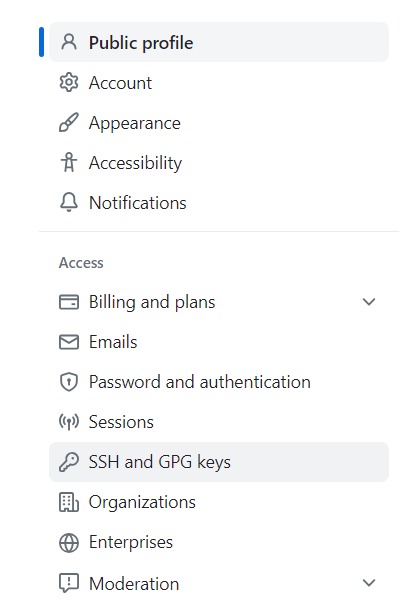
\includegraphics{D:/Users/hayde/Documents/R_sites/Computo_Cientifico/img/github_5.png}
\caption{SSH and GPG Keys}
\end{figure}

Una vez ahí da clic en ``Nueva llave SSH''.

\begin{figure}
\centering
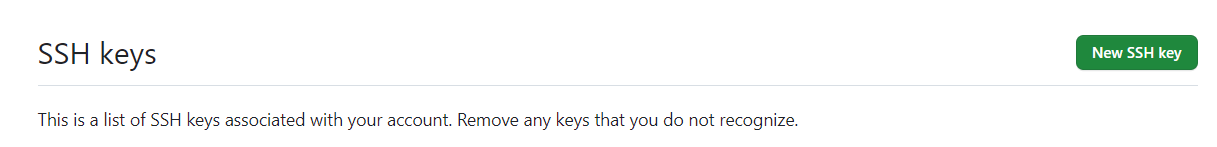
\includegraphics{D:/Users/hayde/Documents/R_sites/Computo_Cientifico/img/github_6.png}
\caption{Nueva llave SSH}
\end{figure}

Después coloca un título que te permita identificar que será la clave con la que usarás la computadora y pega tu llave pública.

\begin{figure}
\centering
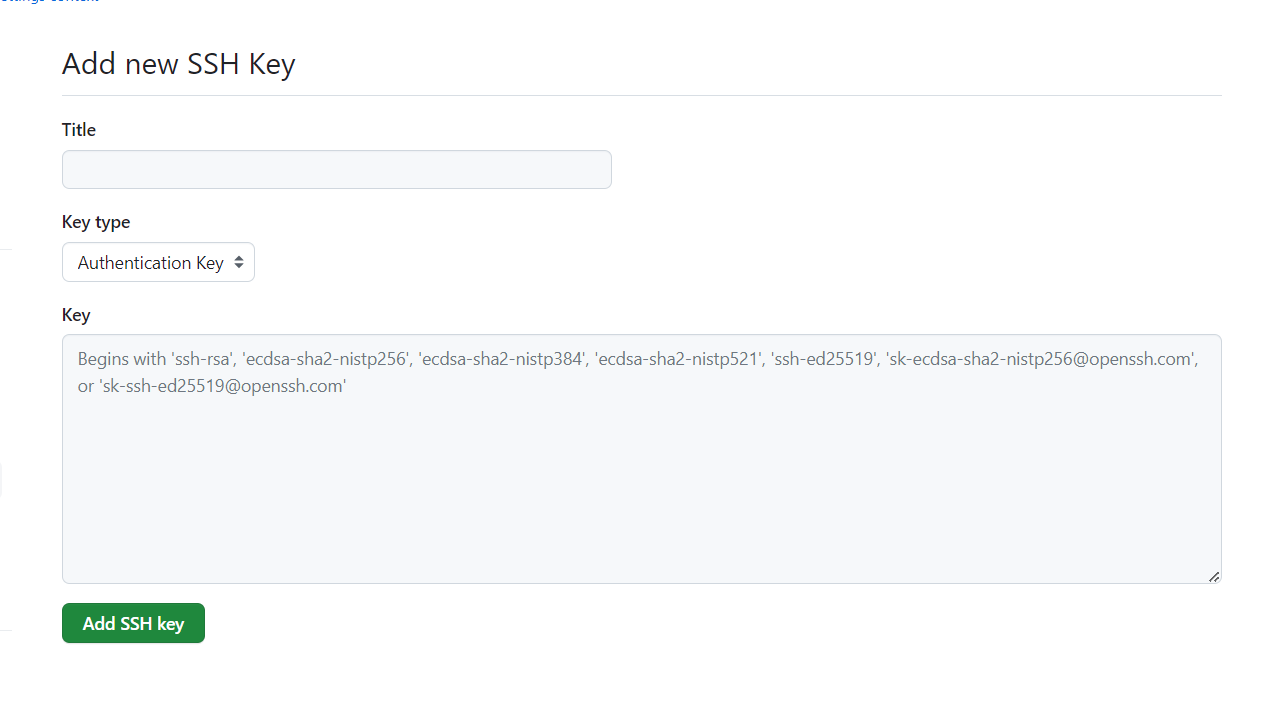
\includegraphics{D:/Users/hayde/Documents/R_sites/Computo_Cientifico/img/github_7.png}
\caption{Llave pública}
\end{figure}

Ahora solo falta revisar la conexión desde la terminal.

\begin{Shaded}
\begin{Highlighting}[]
\ExtensionTok{$}\NormalTok{ ssh }\AttributeTok{{-}T}\NormalTok{ git@github.com}
\end{Highlighting}
\end{Shaded}

Si vez un mensaje similar al siguiente, significa que quedo completa la autenticación.

\begin{Shaded}
\begin{Highlighting}[]
\ExtensionTok{$}\NormalTok{ Hi Name! Youve successfully authenticated, but GitHub does not provide shell access.}
\end{Highlighting}
\end{Shaded}

\hypertarget{paso-4-push-and-pull}{%
\subsection{Paso 4: Push and pull}\label{paso-4-push-and-pull}}

Una vez que ya tenemos configurado todo, solo falta enviar todo lo que tenemos en el repo local al remoto. Si se establecio la contraseña nos la va a pedir en la terminal o una ventana aparte.

\begin{Shaded}
\begin{Highlighting}[]
\ExtensionTok{$}\NormalTok{ git push origin main}
\end{Highlighting}
\end{Shaded}

En esa instrucción, \texttt{origin} se refiere al repositorio remoto y \texttt{main} al local (las ramas que estamos intentando poner en el mismo contenido).

La situación en la que estamos es la siguiente:

\begin{figure}
\centering
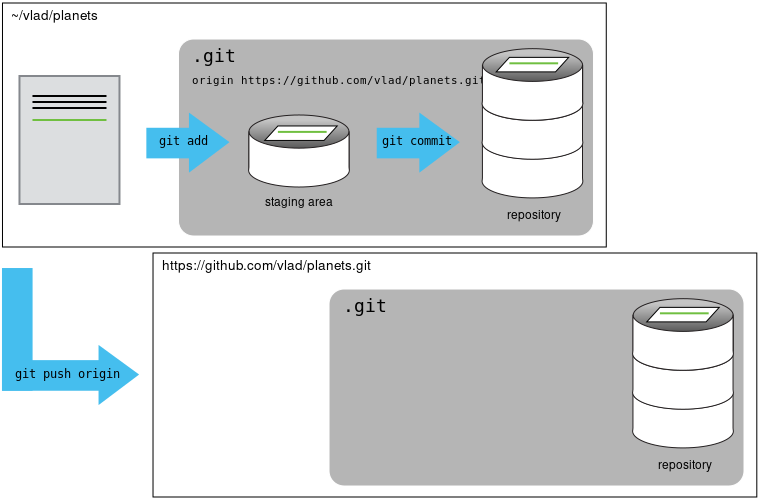
\includegraphics{D:/Users/hayde/Documents/R_sites/Computo_Cientifico/img/github-repo-after-first-push.png}
\caption{\texttt{git\ push\ origin\ main}}
\end{figure}

Para actualizar nuestro repositorio local, lo que debemos hacer es lo siguiente:

\begin{Shaded}
\begin{Highlighting}[]
\ExtensionTok{$}\NormalTok{ git pull origin main}
\end{Highlighting}
\end{Shaded}

Como no hemos realizado ningún cambio en el remoto, no veremos nada nuevo en el local. En el remoto también podemos añadir archivos directamente.

\textbf{Ejercicio:} Añade un archivo nuevo desde el repositorio remoto y actualiza tus cambios en el local.

\hypertarget{colaboradores}{%
\section{Colaboradores}\label{colaboradores}}

Para esta parte, vamos a trabajar en parejas (si no es posible pueden abrir una segunda terminal para la realizar la parte de su equipo).

Vamos a ir a nuestro repositorio que creamos en GitHub y vamos a ir a la configuración y después en donde dice colaboradores.

\begin{figure}
\centering
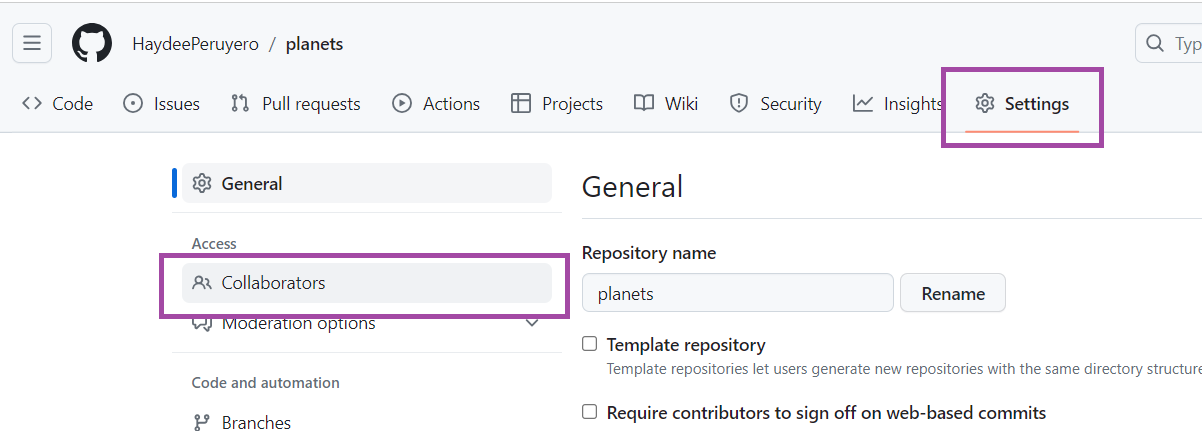
\includegraphics{D:/Users/hayde/Documents/R_sites/Computo_Cientifico/img/github_8.png}
\caption{Configurar colaboradores}
\end{figure}

Una vez en esa ventana, den clic en añadir colaboradores. Van a buscar con el nombre de usuario de su compañero y dan enter.

\begin{figure}
\centering
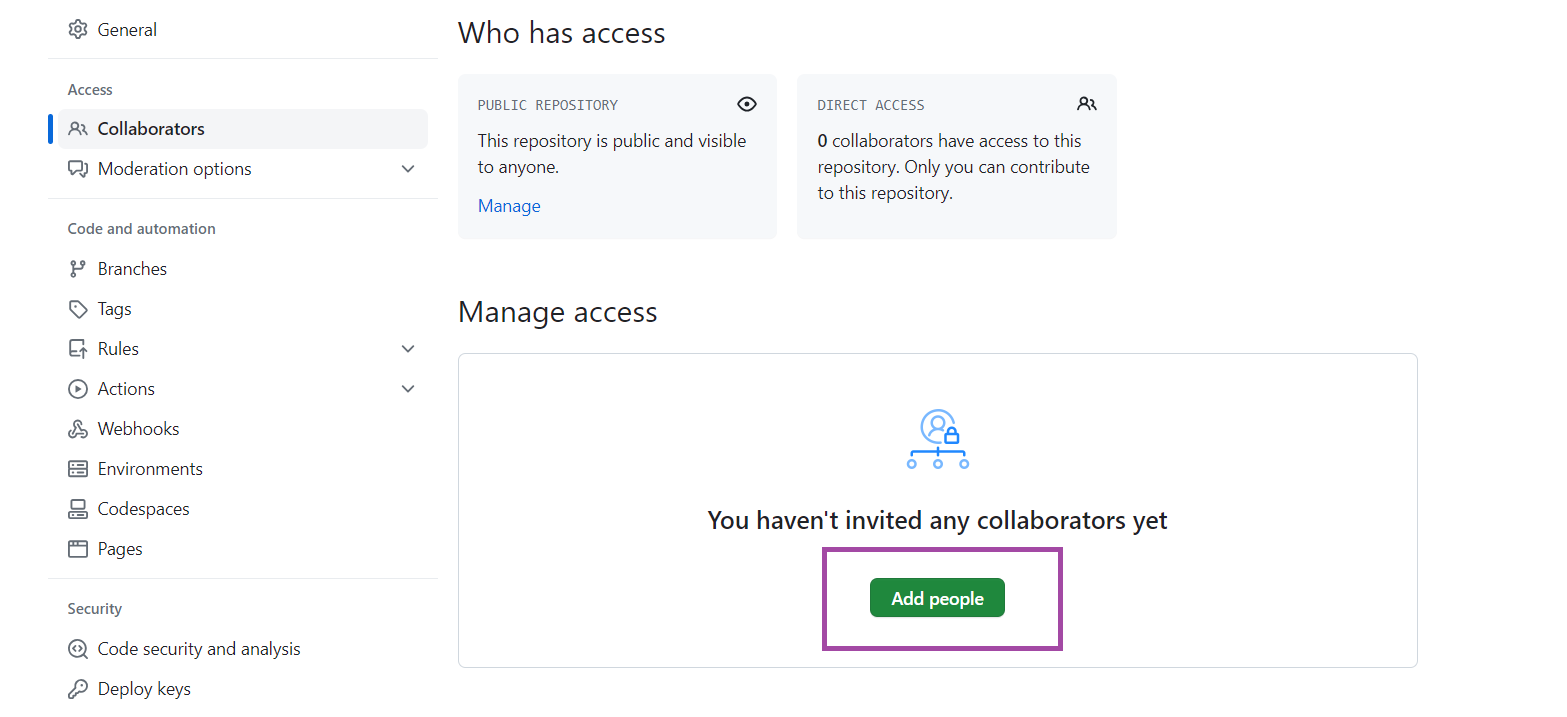
\includegraphics{D:/Users/hayde/Documents/R_sites/Computo_Cientifico/img/github_9.png}
\caption{Añadir colaboradores}
\end{figure}

En su correo o cuenta de github, deben ir a notificaciones y aceptar la invitación. También pueden usar el \href{https://github.com/notifications}{link}.

Ahora, su colaborador debe descargar el repositorio a su computadora, a este paso se le llama clonar un repositorio. Para esto, abran una terminal y realicen lo siguiente:

\begin{Shaded}
\begin{Highlighting}[]
\ExtensionTok{$}\NormalTok{ git clone git@github.com:User/Mi\_primer\_repo.git \textasciitilde{}/colaborador{-}Mi\_primer\_repo}
\end{Highlighting}
\end{Shaded}

La última parte de esa instrucción es la dirección de su computadora donde se clonara el repositorio de su colaborador.

\begin{figure}
\centering
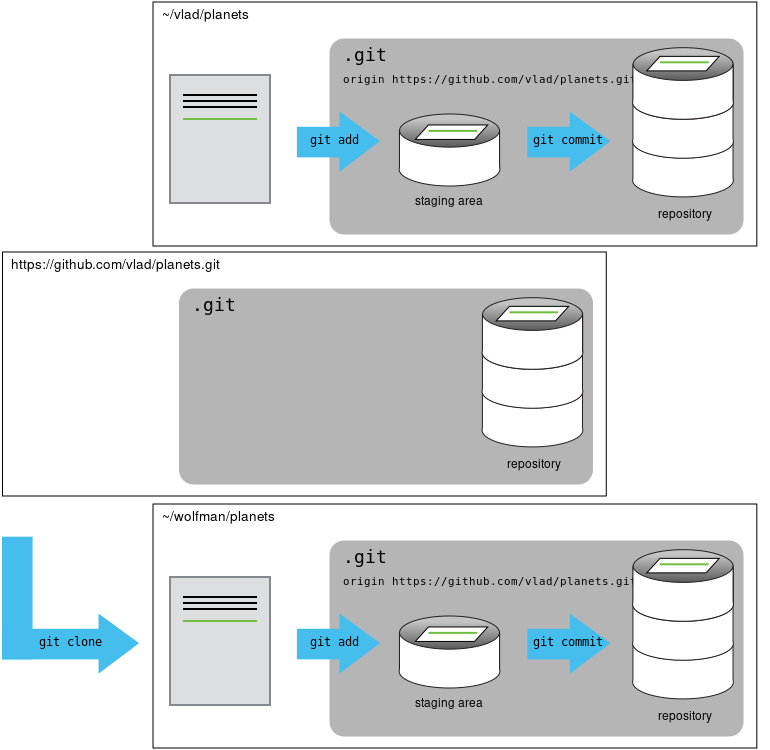
\includegraphics{D:/Users/hayde/Documents/R_sites/Computo_Cientifico/img/github-collaboration.png}
\caption{Estructura de los repositorios al clonarlos. Imagen de \href{https://swcarpentry.github.io/git-novice/08-collab.html}{SC}}
\end{figure}

Ahora, el colaborador realizará un cambio en el repositorio. Para esto, creará un archivo, lo añadira al área de preparación, hará el commit correspondiente y enviará los cambios al remoto.

\begin{Shaded}
\begin{Highlighting}[]
\ExtensionTok{$}\NormalTok{ nano notas.txt}
\ExtensionTok{$}\NormalTok{ git add notas.txt}
\ExtensionTok{$}\NormalTok{ git commit }\AttributeTok{{-}m} \StringTok{"Añadimos archivo de colaborador"}
\ExtensionTok{$}\NormalTok{ git push origin main}
\end{Highlighting}
\end{Shaded}

Si revisamos en la página de Github, veremos ahora un cambio en el repositorio, junto con el commit y quien lo realizo. Finalmente, actualizaremos el repositorio original local con los cambios del colaborador.

\begin{Shaded}
\begin{Highlighting}[]
\ExtensionTok{$}\NormalTok{ git pull origin main}
\end{Highlighting}
\end{Shaded}

Una buena practica cuando se trabaja con colaboradores es realizar la siguiente serie de pasos:

\begin{enumerate}
\def\labelenumi{\arabic{enumi})}
\item
  Antes de comenzar a trabajar, siempre actualizar nuestro repositorio local con \texttt{git\ pull\ origin\ main}
\item
  Realizar cambios y añadirlos al área de preparación con \texttt{git\ add}
\item
  Realizar el commit con un mensaje apropiado que nos permita detectar que cambio se realizó.
\item
  Actualizar el repositorio remoto con los cambios usando \texttt{git\ push\ origin\ main}.
\end{enumerate}

Otra buena practica es trabajar con ramas, este sería un paso antes del 2.

\textbf{Ejercicio:} Replicar lo que se hizo en esta sección cambiando roles de quien es el colaborador y quien el dueño del repositorio local.

\hypertarget{conflictos}{%
\section{Conflictos}\label{conflictos}}

Cuando comenzamos a trabajar con colaboradores, es usual que generemos conflictos si no se trabaja de forma adecuada.

Vamos a crear un conflicto para después resolverlo.

El colaborador va a modificar el \texttt{notas.txt} añadiendo algo. Luego lo añadirá al área de preparación, realizará el commit correspondiente y finalmente actualizará el repositorio remoto.

\begin{Shaded}
\begin{Highlighting}[]
\ExtensionTok{$}\NormalTok{ nano notas.txt}
\ExtensionTok{$}\NormalTok{ git add notas.txt}
\ExtensionTok{$}\NormalTok{ git commit }\AttributeTok{{-}m} \StringTok{"Modificamos el archivo notas para crear un conflicto"}
\ExtensionTok{$}\NormalTok{ git push origin main}
\end{Highlighting}
\end{Shaded}

Ahora, el dueño del repositorio realizará un cambio también al archivo notas (sin antes actualizar con los últimos cambios del colaborador) y realizará todos los pasos hasta poder actualizar el repositorio remoto.

\begin{Shaded}
\begin{Highlighting}[]
\ExtensionTok{$}\NormalTok{ nano notas.txt}
\ExtensionTok{$}\NormalTok{ git add notas.txt}
\ExtensionTok{$}\NormalTok{ git commit }\AttributeTok{{-}m} \StringTok{"Cambios en el archivo notas por el dueño del repositorio"}
\ExtensionTok{$}\NormalTok{ git push origin main}
\end{Highlighting}
\end{Shaded}

\begin{figure}
\centering
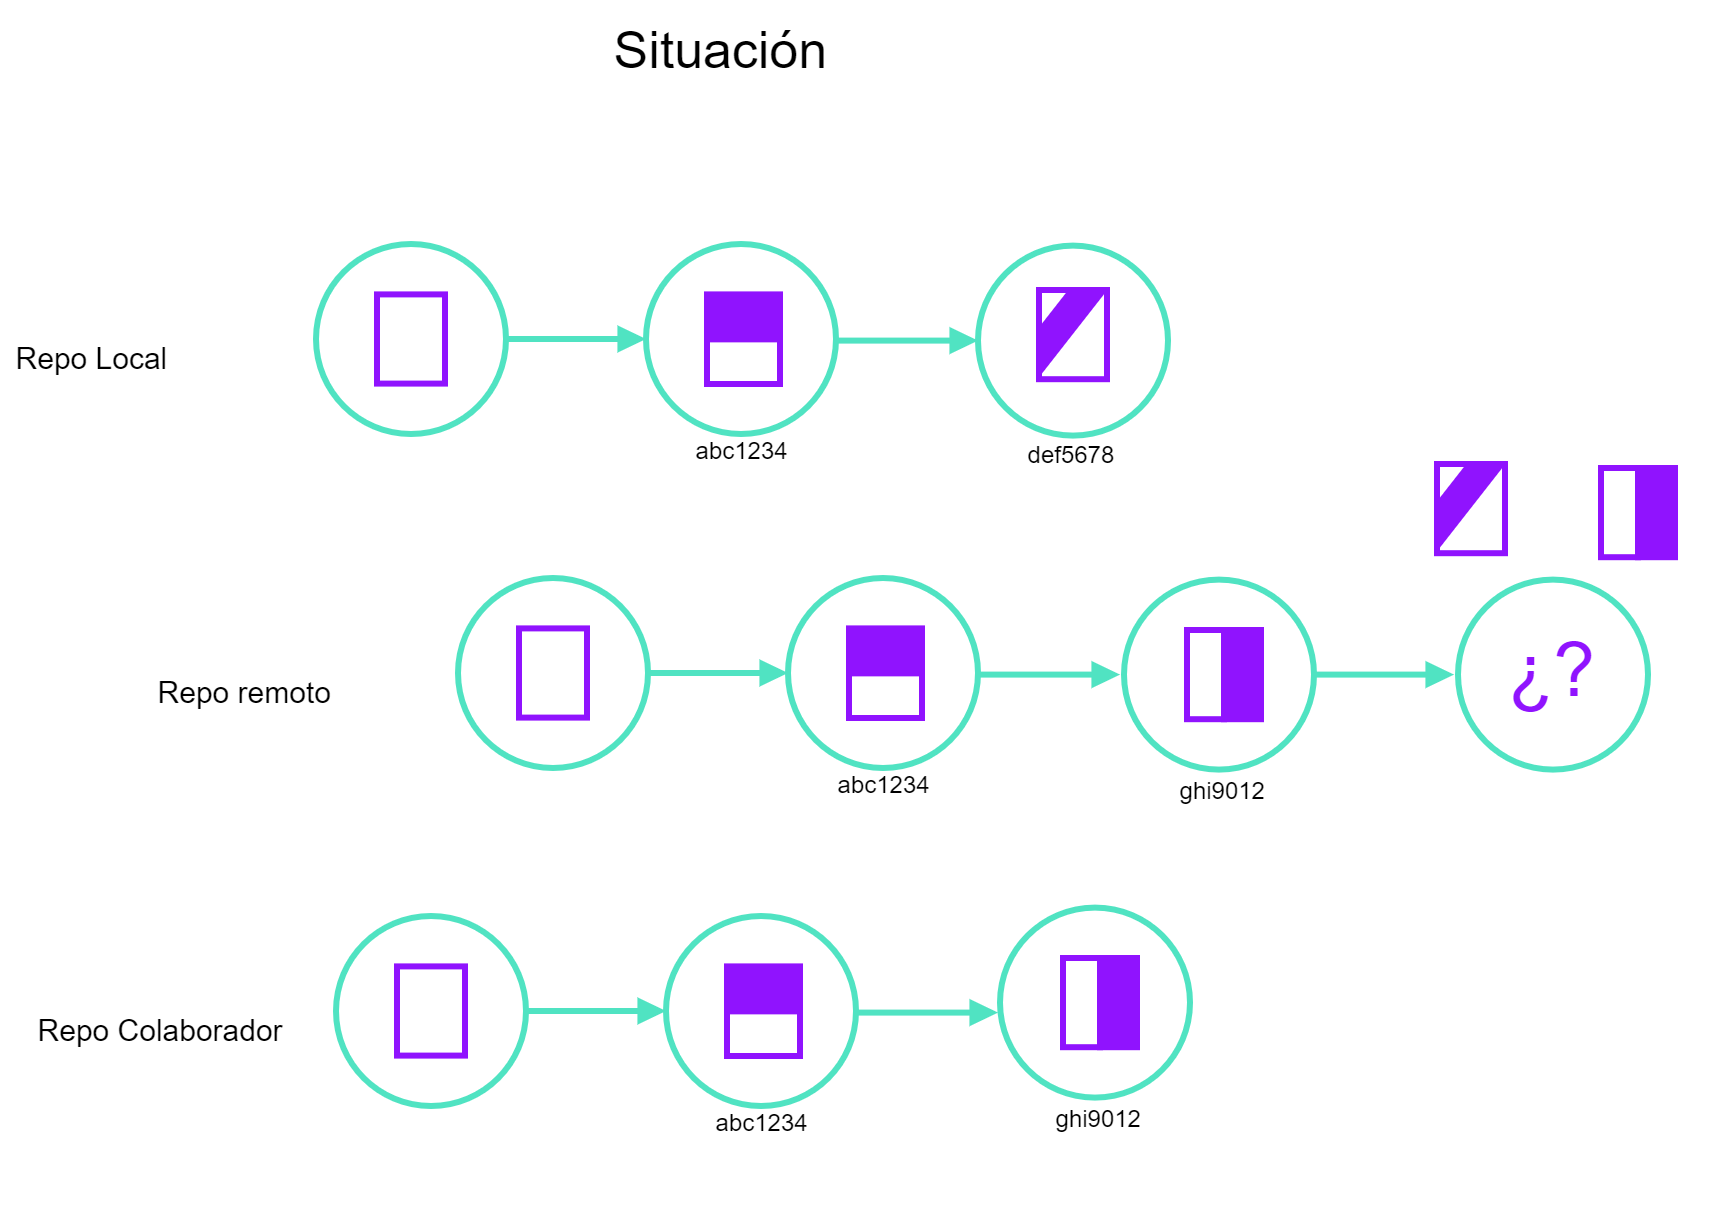
\includegraphics{D:/Users/hayde/Documents/R_sites/Computo_Cientifico/img/git-colaborador-remoto.png}
\caption{Conflicto generado cuando se intenta hacer un \texttt{git\ push}}
\end{figure}

Git no autorizo hacer el push porque había cambios en el remoto que no habíamos actualizado en el local, entonces vamos a actualizar el local primero, hacer un merge en la copia en la que estamos trabajando y después ya hacer un push.

\begin{Shaded}
\begin{Highlighting}[]
\ExtensionTok{$}\NormalTok{ git pull origin main}
\end{Highlighting}
\end{Shaded}

Vamos a ver un mensaje de que hay un merge que no pudo resolver porque se trabajo en la misma línea en el mismo archivo. Si abrimos el archivo vamos a ver algo como lo siguiente:

\begin{Shaded}
\begin{Highlighting}[]
\NormalTok{texto aqui}
\NormalTok{\textless{}\textless{}\textless{}\textless{}\textless{}\textless{}\textless{} HEAD}
\NormalTok{cambios locales aqui}
\NormalTok{=======}
\NormalTok{cambios del colaborador aqui}
\NormalTok{\textgreater{}\textgreater{}\textgreater{}\textgreater{}\textgreater{}\textgreater{}\textgreater{} dabb4c8c450e8475aee9b14b4383acc99f42af1d}
\end{Highlighting}
\end{Shaded}

Ahora lo que tenemos que hacer es decidir que cambios queremos conservar, para eso, podemos borrar nuestros cambios, los del colaborador, ambos, o cambiar todo por algo nuevo (y borrar los identificadores de los conflictos).

Una vez finalizado el merge/resolver conflicto, ya podemos añadirlo al área de preparación, realizar el commit y enviarlo al remoto.

\begin{Shaded}
\begin{Highlighting}[]
\ExtensionTok{$}\NormalTok{ git add notas.txt}
\ExtensionTok{$}\NormalTok{ git status}
\ExtensionTok{$}\NormalTok{ git commit }\AttributeTok{{-}m} \StringTok{"Resolvimos el conflicto en el archivo notas"}
\ExtensionTok{$}\NormalTok{ git push origin main}
\end{Highlighting}
\end{Shaded}

Cuando el colaborador intente hacer un \texttt{git\ pull} no verá ningún conflicto ya que git conservo el registro de que se resolvió y a la copia del colaborador se actualizará sin ningún problema.

\begin{Shaded}
\begin{Highlighting}[]
\ExtensionTok{$}\NormalTok{ git pull origin main}
\end{Highlighting}
\end{Shaded}

Una forma de evitar algunos conflictos es trabajando en ramas, o distribuyendo el trabajo y que cada quien trabaje sobre archivos diferentes.

También se puede dar el caso de que los conflictos sean por archivos con el mismo nombre pero con contenidos totalmente diferentes, por ejemplo con imágenes.

Vamos a crear de nuevo un conflicto con una imagen y vamos a tratar de resolverlo. Tanto el colaborador como el dueño del proyecto va a crear una imagen con el nombre imagen\_prueba.jpg, guardará los cambios y realizará todo hasta mandarlo al repositorio remoto.

\begin{Shaded}
\begin{Highlighting}[]
\ExtensionTok{$}\NormalTok{ head }\AttributeTok{{-}c}\NormalTok{ 1024 /dev/urandom }\OperatorTok{\textgreater{}}\NormalTok{ imagen\_prueba.jpg}
\ExtensionTok{$}\NormalTok{ ls }\AttributeTok{{-}lh}\NormalTok{ imagen\_prueba.jpg}
\end{Highlighting}
\end{Shaded}

Lo añadimos al área de preparación, realizamos commit y lo enviamos al repositorio remoto.

\begin{Shaded}
\begin{Highlighting}[]
\ExtensionTok{$}\NormalTok{ git add imagen\_prueba.jpg}
\ExtensionTok{$}\NormalTok{ git commit }\AttributeTok{{-}m} \StringTok{"Se creo imagen random para generar conflicto."}
\end{Highlighting}
\end{Shaded}

El colaborador realizará un push de su imagen al repositorio remoto.

\begin{Shaded}
\begin{Highlighting}[]
\ExtensionTok{$}\NormalTok{ git push origin main}
\end{Highlighting}
\end{Shaded}

Ahora el dueño del repositorio tratará de hacer un push también al repositorio.

\begin{Shaded}
\begin{Highlighting}[]
\ExtensionTok{$}\NormalTok{ git push origin main}
\end{Highlighting}
\end{Shaded}

Lo primero que nos va a pasar y decir git, es que no actualizamos nuestro repositorio con los cambios como en el ejercicio anterior. Vamos a hacer un pull.

\begin{Shaded}
\begin{Highlighting}[]
\ExtensionTok{$}\NormalTok{ git pull origin main}
\end{Highlighting}
\end{Shaded}

Nos va a marcar que hay conflictos y que no puede hacer auto merge y nos dirá adicionalmente un mensaje similar al siguiente:

\begin{Shaded}
\begin{Highlighting}[]
\NormalTok{warning: Cannot merge binary files: imagen\_prueba.jpg (HEAD vs. 439dc8c08869c343538f6dc4a2b615b05b93c76e)}
\end{Highlighting}
\end{Shaded}

Esto se debe a que como es un archivo que no es de texto no puede empalmar los cambios. Entonces las opciones que tenemos es decidir quedarnos con solo una de las dos imágenes o renombrarlas para quedarnos con ambos.

\begin{enumerate}
\def\labelenumi{\arabic{enumi})}
\tightlist
\item
  Quedarnos con la imagen del dueño del repo:
\end{enumerate}

La imagen del dueño del repo es el HEAD y la del colaborador tiene un id de commit. Entonces procedemos a lo siguiente.

\begin{Shaded}
\begin{Highlighting}[]
\ExtensionTok{$}\NormalTok{ git checkout HEAD imagen\_prueba.jpg}
\ExtensionTok{$}\NormalTok{ git add imagen\_prueba.jpg}
\ExtensionTok{$}\NormalTok{ git commit }\AttributeTok{{-}m} \StringTok{"Usar la imagen del dueño del repo en lugar de la del colaborador"}
\end{Highlighting}
\end{Shaded}

\begin{enumerate}
\def\labelenumi{\arabic{enumi})}
\setcounter{enumi}{1}
\tightlist
\item
  Quedarnos con la imagen del colaborador del repo:
\end{enumerate}

La imagen del colaborador tiene un id de commit, buscarlo. Entonces procedemos a lo siguiente.

\begin{Shaded}
\begin{Highlighting}[]
\ExtensionTok{$}\NormalTok{ git checkout 439dc8c0 imagen\_prueba.jpg}
\ExtensionTok{$}\NormalTok{ git add imagen\_prueba.jpg}
\ExtensionTok{$}\NormalTok{ git commit }\AttributeTok{{-}m} \StringTok{"Usar la imagen del colaborador del repo en lugar de la del dueño"}
\end{Highlighting}
\end{Shaded}

\begin{enumerate}
\def\labelenumi{\arabic{enumi})}
\setcounter{enumi}{2}
\tightlist
\item
  Quedarnos con ambas imágenes:
\end{enumerate}

\begin{Shaded}
\begin{Highlighting}[]
\FunctionTok{git}\NormalTok{ checkout HEAD imagen\_prueba.jpg}
\ExtensionTok{$}\NormalTok{ git mv imagen\_prueba.jpg imagen\_prueba{-}dueño.jpg}
\ExtensionTok{$}\NormalTok{ git checkout 439dc8c0 imagen\_prueba.jpg}
\ExtensionTok{$}\NormalTok{ mv imagen\_prueba.jpg imagen\_prueba{-}colaborador.jpg}
\end{Highlighting}
\end{Shaded}

Y finalmente para remover la imagen de prueba y añadir las dos nuevas versiones:

\begin{Shaded}
\begin{Highlighting}[]
\ExtensionTok{$}\NormalTok{ git rm imagen\_prueba.jpg}
\ExtensionTok{$}\NormalTok{ git add imagen\_prueba{-}dueño.jpg}
\ExtensionTok{$}\NormalTok{ git add imagen\_prueba{-}colaborador.jpg}
\ExtensionTok{$}\NormalTok{ git commit }\AttributeTok{{-}m} \StringTok{"Use two images: dueño y colaborador"}
\ExtensionTok{$}\NormalTok{ git push origin main}
\end{Highlighting}
\end{Shaded}

\hypertarget{trabajando-con-ramas}{%
\section{Trabajando con Ramas}\label{trabajando-con-ramas}}

Trabajar con ramas en Git es una parte fundamental del flujo de trabajo colaborativo. Los siguientes pasos son los básicos para trabajar de esta manera.

\hypertarget{crear-una-rama}{%
\subsection{1. Crear una rama}\label{crear-una-rama}}

Cuando trabajas en un proyecto, es una buena práctica crear una rama separada para cada nueva función o corrección de errores que estés desarrollando. Para crear una nueva rama en Git, utiliza el comando:

\begin{Shaded}
\begin{Highlighting}[]
\ExtensionTok{$}\NormalTok{ git checkout }\AttributeTok{{-}b}\NormalTok{ nombre\_de\_la\_rama}
\end{Highlighting}
\end{Shaded}

Este comando crea una nueva rama y te cambia a ella al mismo tiempo.

Otra opción es la siguiente:

\begin{Shaded}
\begin{Highlighting}[]
\ExtensionTok{$}\NormalTok{ git branch nombre\_de\_la\_rama}
\ExtensionTok{$}\NormalTok{ git switch nombre\_de\_la\_rama}
\end{Highlighting}
\end{Shaded}

\hypertarget{trabajar-en-la-rama}{%
\subsection{2. Trabajar en la rama}\label{trabajar-en-la-rama}}

Después de crear la rama, puedes comenzar a trabajar en tus cambios. Realiza tus modificaciones en los archivos como lo harías normalmente.

\hypertarget{agregar-y-confirmar-cambios}{%
\subsection{3. Agregar y confirmar cambios}\label{agregar-y-confirmar-cambios}}

Una vez que hayas realizado cambios que desees incluir en la rama, añádelos al área de preparación con:

\begin{Shaded}
\begin{Highlighting}[]
\ExtensionTok{$}\NormalTok{ git add nombre\_del\_archivo}
\end{Highlighting}
\end{Shaded}

Luego, confirma los cambios con un mensaje descriptivo:

\begin{Shaded}
\begin{Highlighting}[]
\ExtensionTok{$}\NormalTok{ git commit }\AttributeTok{{-}m} \StringTok{"Mensaje descriptivo de los cambios"}
\end{Highlighting}
\end{Shaded}

\hypertarget{empujar-la-rama-al-repositorio-remoto}{%
\subsection{4. Empujar la rama al repositorio remoto}\label{empujar-la-rama-al-repositorio-remoto}}

Si estás trabajando en un repositorio remoto compartido con otros colaboradores, es posible que desees compartir tus cambios. Para esto, hay dos formas de hacerlo. La primera es enviar los cambios a una rama remota y después confirmarlos y unirlos, para eso utiliza el comando:

\begin{Shaded}
\begin{Highlighting}[]
\ExtensionTok{$}\NormalTok{ git push origin nombre\_de\_la\_rama}
\end{Highlighting}
\end{Shaded}

Esto enviará la nueva rama y los cambios asociados al repositorio remoto.

\hypertarget{fusionar-cambios}{%
\subsection{5. Fusionar cambios}\label{fusionar-cambios}}

Una vez que hayas completado tus cambios y estés listo para incorporarlos al proyecto principal, puedes fusionar tu rama con la rama principal (generalmente \texttt{main} o \texttt{master}). Para hacerlo, primero cámbiate a la rama principal:

\begin{Shaded}
\begin{Highlighting}[]
\ExtensionTok{$}\NormalTok{ git checkout main}
\end{Highlighting}
\end{Shaded}

Otra opción:

\begin{Shaded}
\begin{Highlighting}[]
\ExtensionTok{$}\NormalTok{ git switch main}
\end{Highlighting}
\end{Shaded}

Luego, fusiona tu rama con la rama principal:

\begin{Shaded}
\begin{Highlighting}[]
\ExtensionTok{$}\NormalTok{ git merge nombre\_de\_la\_rama}
\end{Highlighting}
\end{Shaded}

\textbf{NOTA:} Los pasos 4 y 5 se pueden intercambiar de orden, es decir primero hacer el merge local cambiandonos a la rama principal y después enviando los cambios al remoto. Es importante primero hacer un \texttt{git\ pull} para actualizar nuestro local en la rama principal.

\hypertarget{resolver-conflictos-si-los-hay}{%
\subsection{6. Resolver conflictos (si los hay)}\label{resolver-conflictos-si-los-hay}}

Es posible que ocurran conflictos durante el proceso de fusión si otros colaboradores han realizado cambios en las mismas partes de los archivos. Git te indicará los conflictos y te permitirá resolverlos manualmente.

\hypertarget{eliminar-la-rama-opcional}{%
\subsection{7. Eliminar la rama (opcional)}\label{eliminar-la-rama-opcional}}

Una vez que hayas fusionado tus cambios en la rama principal y ya no necesites la rama de la función, puedes eliminarla:

\begin{Shaded}
\begin{Highlighting}[]
\ExtensionTok{$}\NormalTok{ git branch }\AttributeTok{{-}d}\NormalTok{ nombre\_de\_la\_rama}
\end{Highlighting}
\end{Shaded}

\hypertarget{actualizar-y-sincronizar}{%
\subsection{8. Actualizar y sincronizar}\label{actualizar-y-sincronizar}}

Es importante mantener tu repositorio local actualizado con los cambios de otros colaboradores. Para hacerlo, utiliza:

\begin{Shaded}
\begin{Highlighting}[]
\ExtensionTok{$}\NormalTok{ git pull origin main}
\end{Highlighting}
\end{Shaded}

Esto traerá los últimos cambios de la rama principal del repositorio remoto y los fusionará con tu rama local.

Siguiendo estos pasos, podrás trabajar de manera efectiva con ramas en Git en un entorno colaborativo. Recuerda comunicarte con tus colaboradores y mantener un flujo de trabajo ordenado para evitar conflictos y errores.

\hypertarget{conectar-con-overleaf}{%
\section{Conectar con overleaf}\label{conectar-con-overleaf}}

Lo primero es crear el documento en Overleaf que nos interesa. Después se clona el archivo con la dirección que da Overleaf. Esa será la ruta de la carpeta. De manera local podemos cambiar el propio archivo \emph{.tex} por uno que ya tengamos (parece que es más fácil hacer esto que intentar crear un nuevo documento en Overleaf a partir un repositorio existente, pero falta hacer más pruebas); también, es posible cambiar el nombre de la carpeta en la cual se generó el repositorio (parece que no hay problemas con Overleaf pero hay que hacer más pruebas).

A continuación los pasos para trabajar localmente una vez que ya se tiene el repositorio creado.

\begin{enumerate}
\def\labelenumi{\arabic{enumi})}
\item
  \texttt{cd\ ruta\_de\_la\_carpeta}
\item
  \texttt{git\ branch\ nombre\_rama\_local}
\item
  \texttt{git\ switch\ nombre\_rama\_local} (o master)
\item
  \texttt{git\ status} (para ver cambios)
\item
  \texttt{git\ add\ .} (para añadir los cambios-todos)
\item
  `git commit -m ``nombre del mensaje''``
\item
  \texttt{git\ switch\ master}
\item
  \texttt{git\ pull}
\item
  \texttt{git\ merge\ nombre\_rama\_local}
\end{enumerate}

\begin{enumerate}
\def\labelenumi{(\alph{enumi})}
\tightlist
\item
  \texttt{git\ switch\ nombre\_rama\_local}
  (b) \texttt{git\ merge\ master} (para actualizar ahora rama local)
  (c) seguir trabajando sobre la misma rama local
  (d) repetir de 4 a 9
\end{enumerate}

\begin{enumerate}
\def\labelenumi{\arabic{enumi})}
\setcounter{enumi}{9}
\item
  \texttt{git\ push}
\item
  \texttt{git\ branch\ -d\ nombre\_rama\_local}
\end{enumerate}

\hypertarget{python}{%
\chapter{Python}\label{python}}

\hypertarget{tipos-de-datos}{%
\section{Tipos de datos}\label{tipos-de-datos}}

\hypertarget{flujo-de-control}{%
\section{Flujo de control}\label{flujo-de-control}}

\hypertarget{visualizaciuxf3n-de-datos}{%
\section{Visualización de datos}\label{visualizaciuxf3n-de-datos}}

\hypertarget{manipulaciuxf3n-de-bases-de-datos}{%
\section{Manipulación de bases de datos}\label{manipulaciuxf3n-de-bases-de-datos}}

\hypertarget{anuxe1lisis-exploratorio-de-bases-de-datos}{%
\section{Análisis exploratorio de bases de datos}\label{anuxe1lisis-exploratorio-de-bases-de-datos}}

\hypertarget{funciones-y-scripts}{%
\section{Funciones y scripts}\label{funciones-y-scripts}}

\hypertarget{buenas-practicas}{%
\section{Buenas practicas}\label{buenas-practicas}}

\hypertarget{procesamiento-de-alto-rendimiento}{%
\section{Procesamiento de alto rendimiento}\label{procesamiento-de-alto-rendimiento}}

\hypertarget{programaciuxf3n-en-paralelo}{%
\section{Programación en paralelo}\label{programaciuxf3n-en-paralelo}}

\hypertarget{sql}{%
\chapter{SQL}\label{sql}}

\hypertarget{bases-de-datos-y-manipulaciuxf3n}{%
\section{Bases de datos y manipulación}\label{bases-de-datos-y-manipulaciuxf3n}}

\hypertarget{explorar-datos-categuxf3ricos-y-texto-no-estructurado}{%
\section{Explorar datos categóricos y texto no estructurado}\label{explorar-datos-categuxf3ricos-y-texto-no-estructurado}}

\hypertarget{comparaciuxf3n-con-los-otros-programas}{%
\section{Comparación con los otros programas}\label{comparaciuxf3n-con-los-otros-programas}}

\hypertarget{valores-faltantes}{%
\section{Valores faltantes}\label{valores-faltantes}}

\hypertarget{combinar-bases-de-datos}{%
\section{Combinar bases de datos}\label{combinar-bases-de-datos}}

\hypertarget{power-bi}{%
\chapter{Power BI}\label{power-bi}}

\hypertarget{introducciuxf3n-a-power-bi}{%
\section{Introducción a Power BI}\label{introducciuxf3n-a-power-bi}}

\hypertarget{transformando-y-visualizando-datos}{%
\section{Transformando y visualizando datos}\label{transformando-y-visualizando-datos}}

\hypertarget{manipulaciuxf3n-de-bases-de-datos-1}{%
\section{Manipulación de bases de datos}\label{manipulaciuxf3n-de-bases-de-datos-1}}

\hypertarget{anuxe1lisis-exploratorio-de-bases-de-datos-1}{%
\section{Análisis exploratorio de bases de datos}\label{anuxe1lisis-exploratorio-de-bases-de-datos-1}}

\hypertarget{variables-categuxf3ricas-y-continuas}{%
\section{Variables categóricas y continuas}\label{variables-categuxf3ricas-y-continuas}}

\hypertarget{r}{%
\chapter{R}\label{r}}

\hypertarget{tipos-de-datos-1}{%
\section{Tipos de datos}\label{tipos-de-datos-1}}

\hypertarget{manipulaciuxf3n-de-bases-de-datos-2}{%
\section{Manipulación de bases de datos}\label{manipulaciuxf3n-de-bases-de-datos-2}}

\hypertarget{anuxe1lisis-exploratorio-de-bases-de-datos-2}{%
\section{Análisis exploratorio de bases de datos}\label{anuxe1lisis-exploratorio-de-bases-de-datos-2}}

\hypertarget{reportes-con-rmarkdown}{%
\section{Reportes con RMarkdown}\label{reportes-con-rmarkdown}}

\hypertarget{puxe1ginas-web}{%
\section{Páginas web}\label{puxe1ginas-web}}

  \bibliography{book.bib,packages.bib}

\end{document}
